\documentclass[prodmode,acmtosn]{acmsmall}

\usepackage[ruled]{algorithm2e}
\renewcommand{\algorithmcfname}{ALGORITHM}
\SetAlFnt{\small}
\SetAlCapFnt{\small}
\SetAlCapNameFnt{\small}
\SetAlCapHSkip{0pt}
\IncMargin{-\parindent}



%%\usepackage{appendix}
%\usepackage{amssymb}
%\usepackage{algorithm}
%\usepackage{amsmath}
%\usepackage{amssymb}
%\usepackage{array}
%\usepackage{graphicx}
%\usepackage{pifont}
\usepackage{epsfig,tabularx,amssymb,amsmath,subfigure,multirow,booktabs}
%\usepackage{balance}
%\usepackage{bm}
\usepackage[noend]{algpseudocode}
%\usepackage{epsfig,subfigure}
%\usepackage{mathptmx}
%\usepackage{url}
		
\begin{document}

\title{Cooperative Allocation and Scheduling of Tasks for Minimizing  Interval Data Sampling in WSNs}

\author{Yawei~Zhao
\affil{National University of Defense Technology}
Deke~Guo
\affil{National University of Defense Technology}
Jia~Xu
\affil{Guangxi University}
Pin~Lv
\affil{Guangxi University}
Jianping~Yin
\affil{National University of Defense Technology}
}

\begin{abstract}
Data sharing amongst multiple tasks is significant to reduce energy consumption and communication cost in low-power wireless sensor networks. Current proposals have already scheduled the discrete point sampling tasks to decrease the amount of sampled data. However, less effort has been done for the applications requiring continuous interval sampling data. Additionally, most of prior work focuses on scheduling tasks on a single sensor node. In this paper, we broaden the scope to the entire network and attempt to minimize the total amount of interval sampling data instead of traditional discrete point sampling data. Our basic idea is to cooperatively allocate and schedule multiple sampling tasks by utilizing the overlap amongst these tasks. Since the allocation problem is NP-hard and the scheduling problem is NP-complete, we design two dedicated 2-factor approximation methods for task allocation and scheduling, respectively. Extensive real experiments are conducted on a testbed of $50$ sensor nodes to evaluate the effectiveness of our proposals. Moreover, the scalability of our proposals is verified by using the widely-used simulation tool, i.e., TOSSIM. The experimental results indicate that, compared with the state-of-the-art solution, our methods reduce the amount of sampled data significantly.
\end{abstract}

\begin{CCSXML}
<ccs2012>
<concept>
<concept_id>10003033.10003106.10003112.10003238</concept_id>
<concept_desc>Networks~Sensor networks</concept_desc>
<concept_significance>500</concept_significance>
</concept>
<concept>
<concept_id>10002951.10003227.10003236</concept_id>
<concept_desc>Information systems~Spatial-temporal systems</concept_desc>
<concept_significance>300</concept_significance>
</concept>
<concept>
<concept_id>10003033.10003106.10003112</concept_id>
<concept_desc>Networks~Cyber-physical networks</concept_desc>
<concept_significance>100</concept_significance>
</concept>
</ccs2012>
\end{CCSXML}

\ccsdesc[500]{Networks~Sensor networks}
\ccsdesc[300]{Information systems~Spatial-temporal systems}
\ccsdesc[100]{Networks~Cyber-physical networks}


\keywords{Data sharing, interval sampling tasks, data aggregation, coverage, WSNs}

%\acmformat{Yawei Zhao, Deke Guo, Jia Xu, Pin Lv and Jianping Yin, 2015. Cooperative Allocation and Scheduling of Tasks for Minimizing  Interval Data Sampling in WSNs.}

\begin{bottomstuff}
This work is supported by the National Natural Science Foundation of China (NSFC), under Grant 61170287, Grant 61232016, Grant 61402494, Grant 61402513, and Grant 61202487.

Author's addresses: Y. Zhao {and} J. Yin, College of Computer, National University of Defense Technology; D. Guo, Science and Technology on Information System Engineering Laboratory, National University of Defense Technology; J. Xu and P. Lv, School of Computer, Electronics and Information, Guangxi University.
\end{bottomstuff}

\maketitle

\section{Introduction}

\label{introductpion}
Many successful applications of low-power wireless sensor networks (WSNs) under different scenarios, e.g., earthquake monitoring \cite{2005acoustic_diagnose_train}, railway diagnosis \cite{2007sensys_earthquake_monitor}, wild-life protection \cite{2004habitat_monitoring}, and structure monitoring \cite{2004structuralMonitoring}, are time-consuming and labor-intensive. Besides, they are all constrained by multiple scarce resources such as power, memory and computational resources. The experience from some real projects \cite{2009greenorbs,2009_oceansense} shows that the lifetime of an initially deployed WSN is restricted to only a few months without recharging. Therefore, some resource-sharing strategies  are proposed for different applications to improve the efficiency of the WSNs.

Data sharing amongst different applications is such a resource-sharing strategy. It has caught much attention especially for the continuous interval sampling data. Such interval sampling data is derived by performing data sampling for a time interval. For example, acoustic data are continuously collected for a time interval to diagnose the state of the railway system while the discrete data does not help much \cite{2005acoustic_diagnose_train}. As another example, the vibration in the volcano, earthquake \cite{2007sensys_earthquake_monitor} and structure monitoring systems \cite{2004structuralMonitoring} need to be continuously sampled for a period of time to analyze the anomaly while the exceptional data may be lost if the  discrete sampling is employed. A further example is that continuously observed data for a time interval can be utilized to conduct scientific analysis on animals' behaviors \cite{2004habitat_monitoring}. Such an interval sampling task, as shown in Fig. \ref{figure_introduction}, has two properties, namely, a \emph{time window} and a \emph{sampling interval}. The \emph{sampling interval} can be flexibly adjusted in the \emph{time window}, which poses great opportunity to implement data sharing amongst multiple sampling tasks, e.g., the data sharing between tasks $t_2$ and $t_3$ in Fig. \ref{figure_introduction_scheduling}.

\begin{figure}[t]
\centering
\subfigure[Task scheduling]{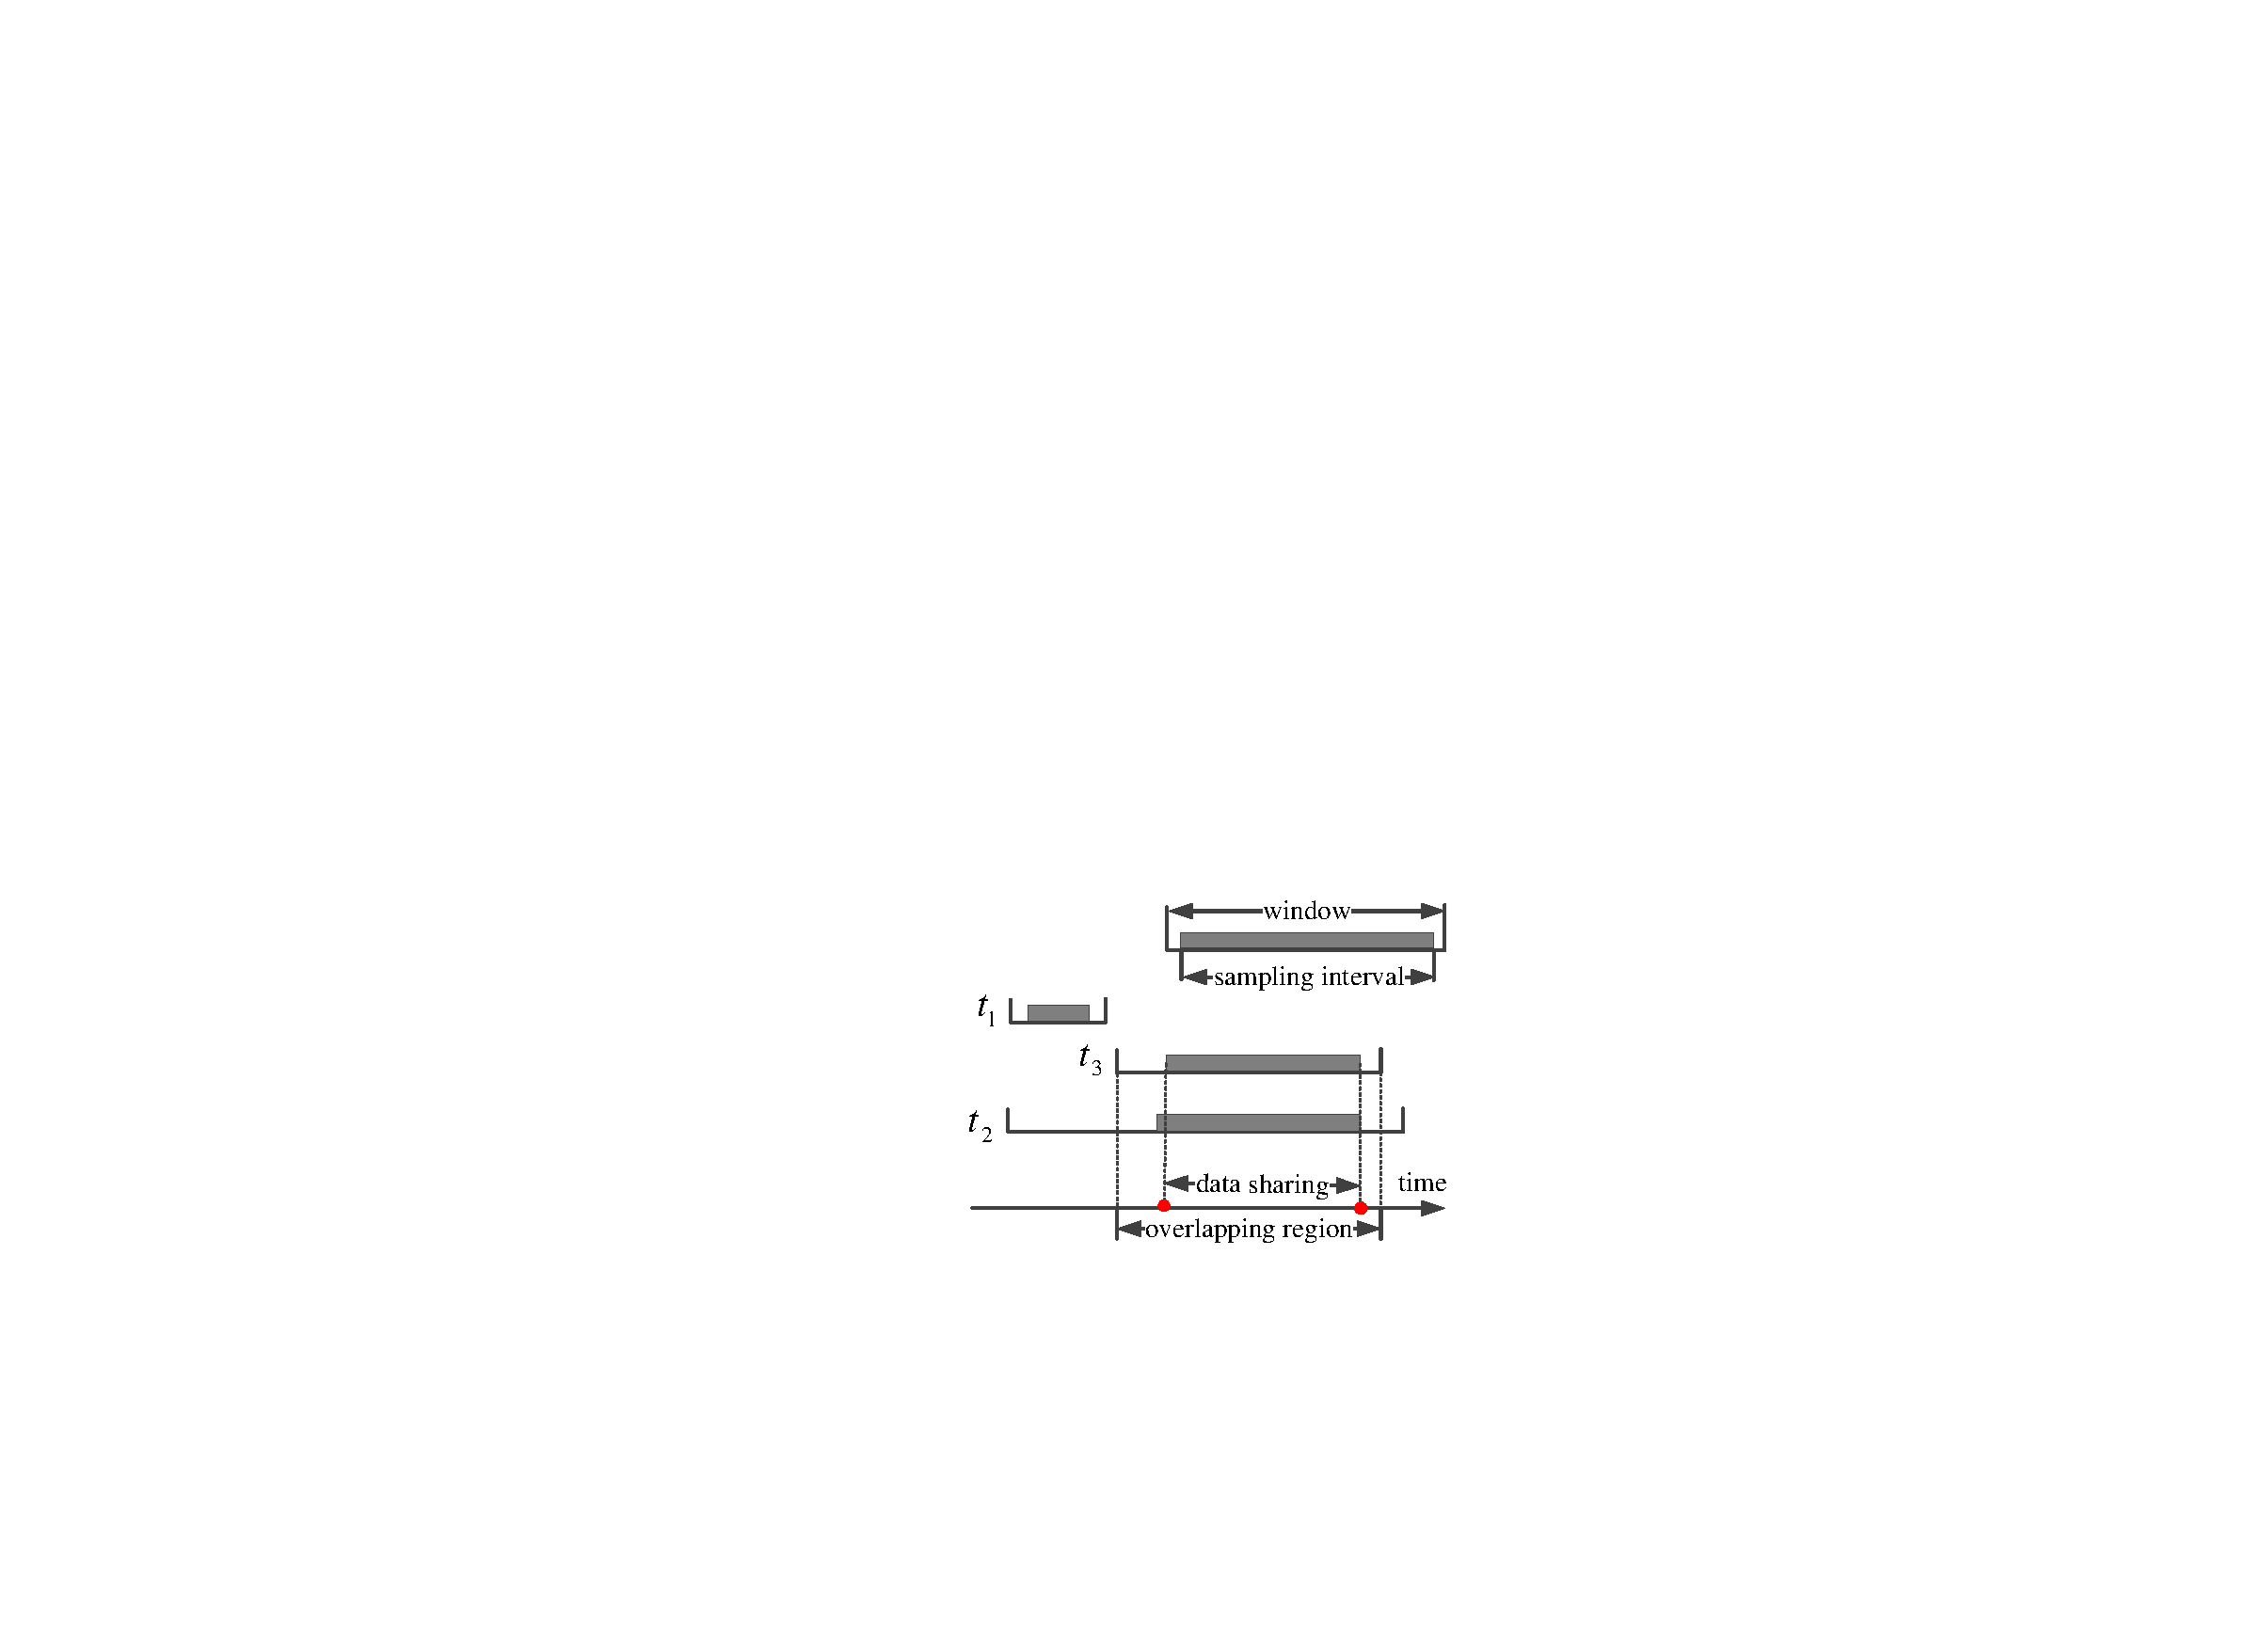
\includegraphics[width=0.33\columnwidth]{Figures/figure_introduction_scheduling}\label{figure_introduction_scheduling}}
\hspace{6pt}
\subfigure[Task allocation]{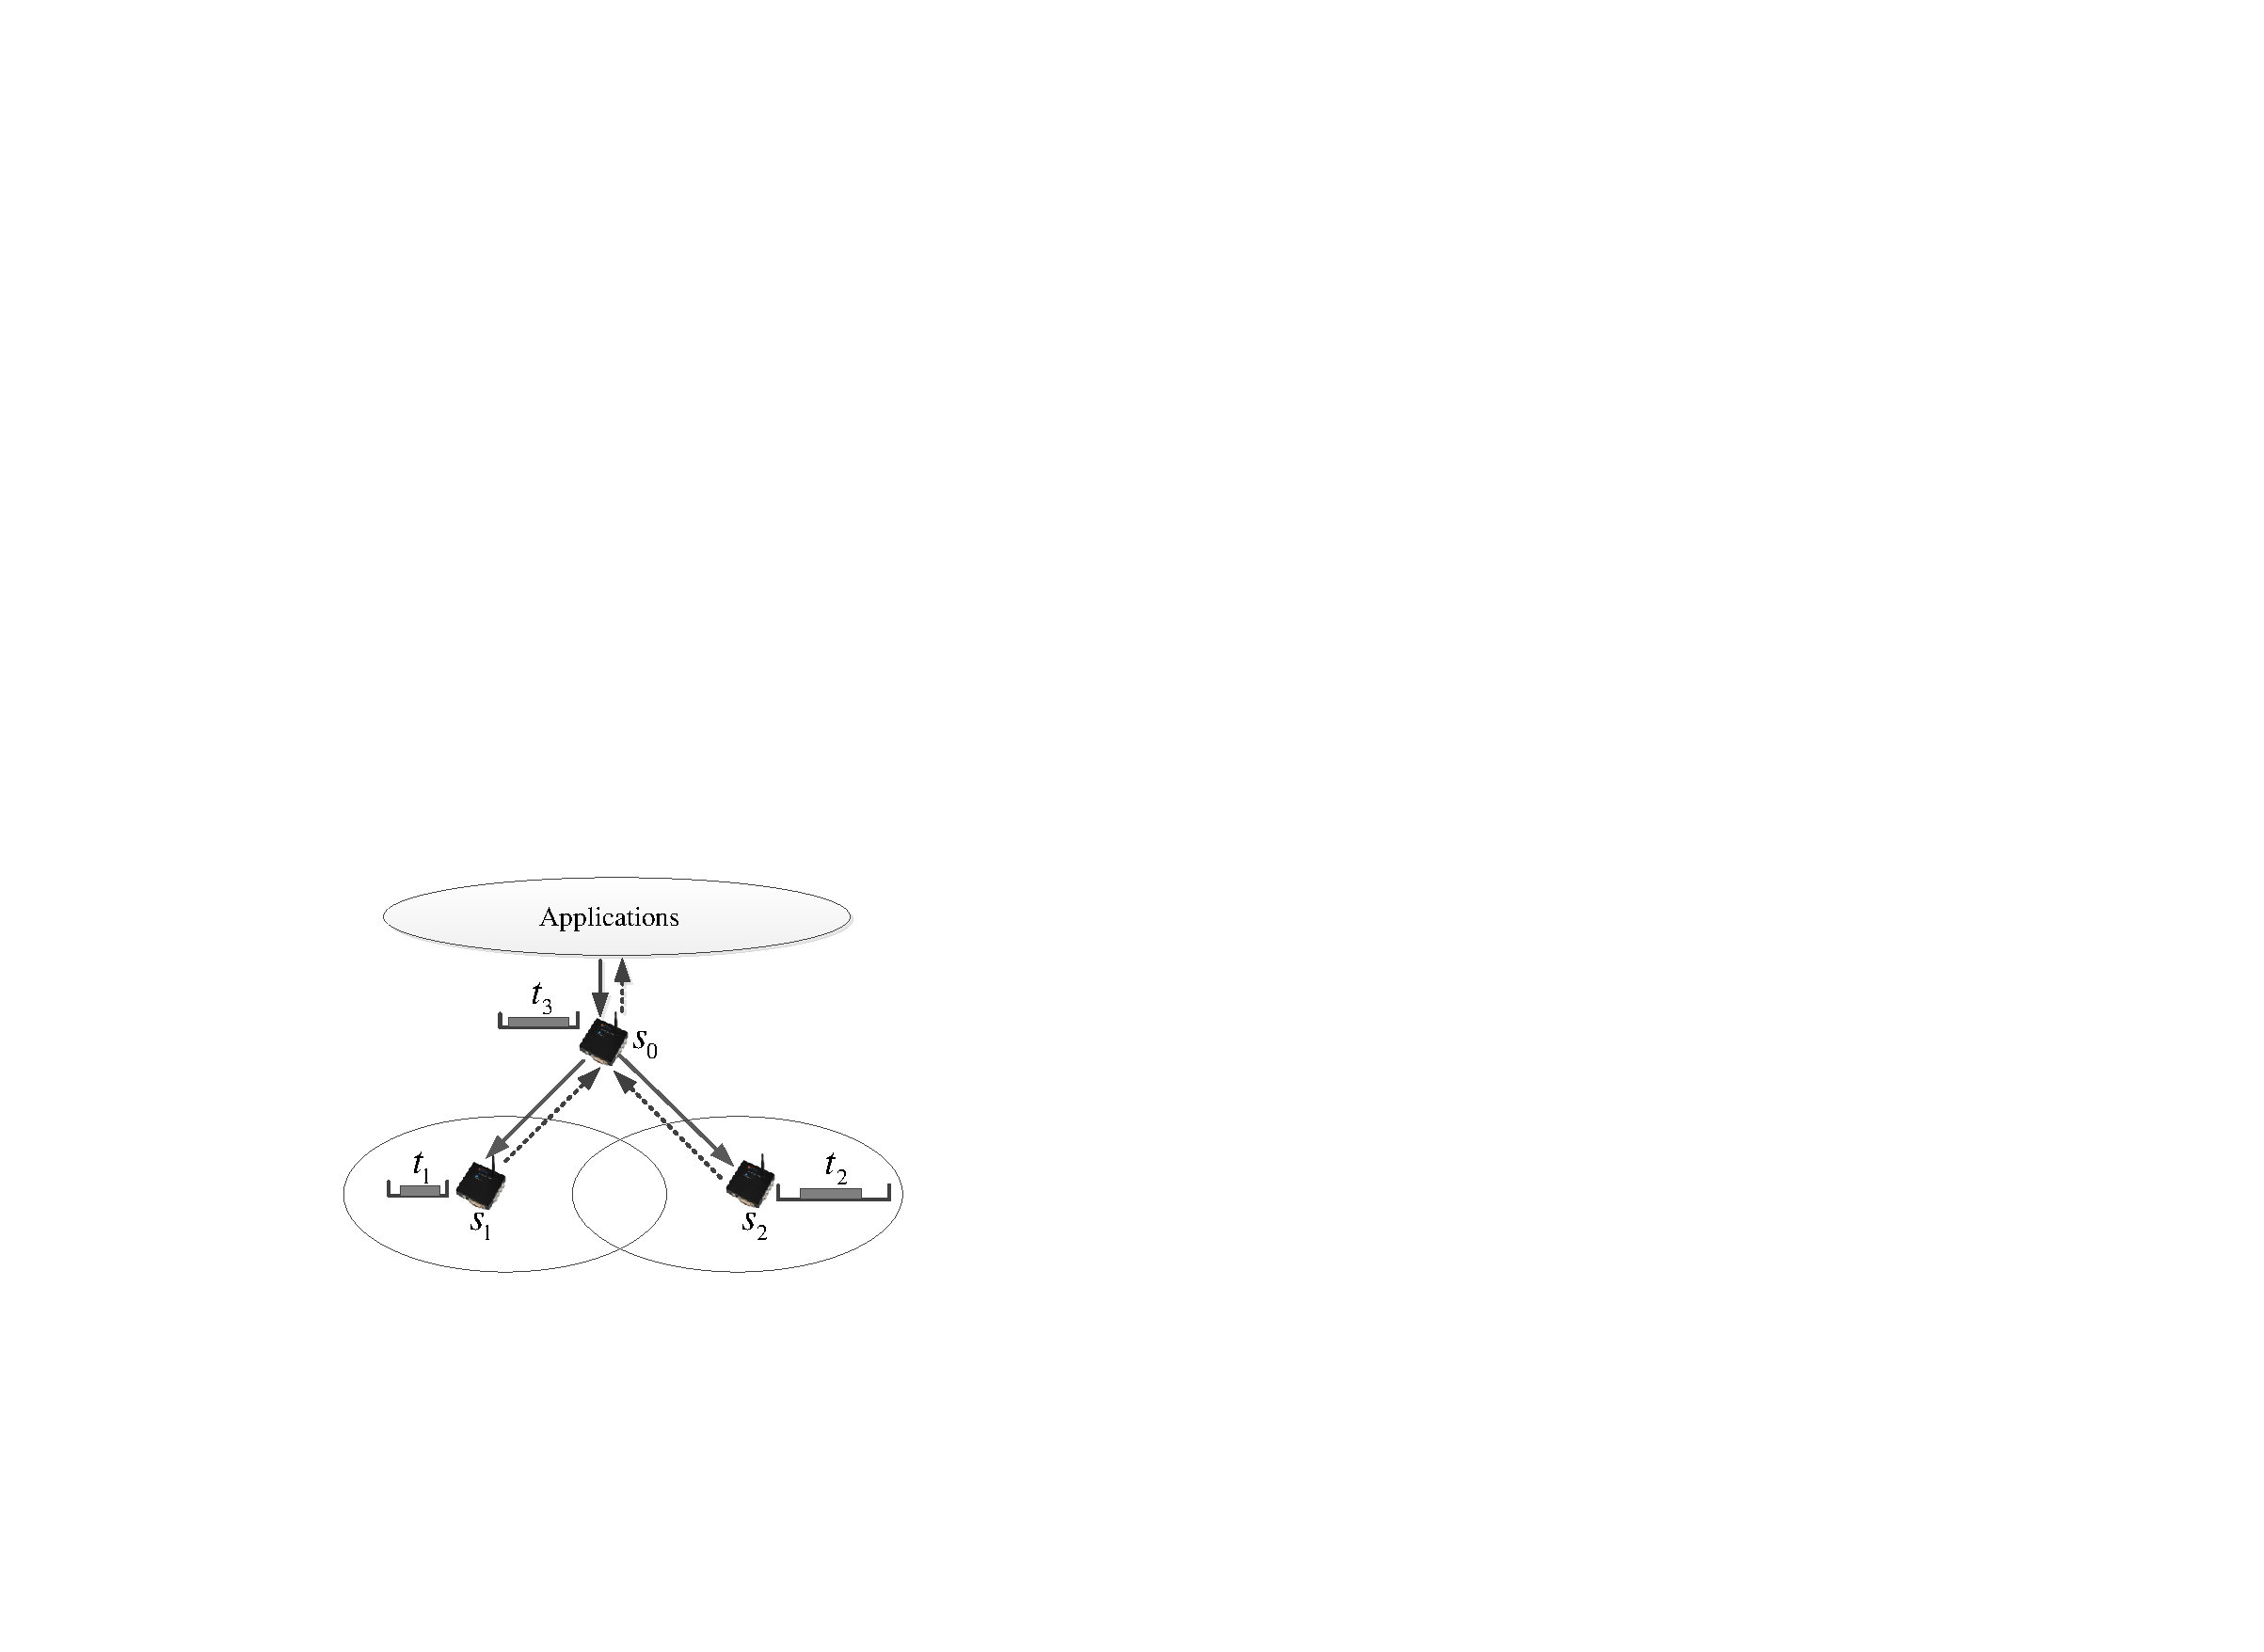
\includegraphics[width=0.4\columnwidth]{Figures/figure_introduction_allocation}\label{figure_introduction_allocation}}
\caption{The illustrative examples for the scheduling of \emph{sampling interval} in the left panel and the allocation of tasks in the right panel.} \label{figure_introduction}
\end{figure}
%\begin{figure}[t]
%\centering
%\subfigure[Task scheduling]{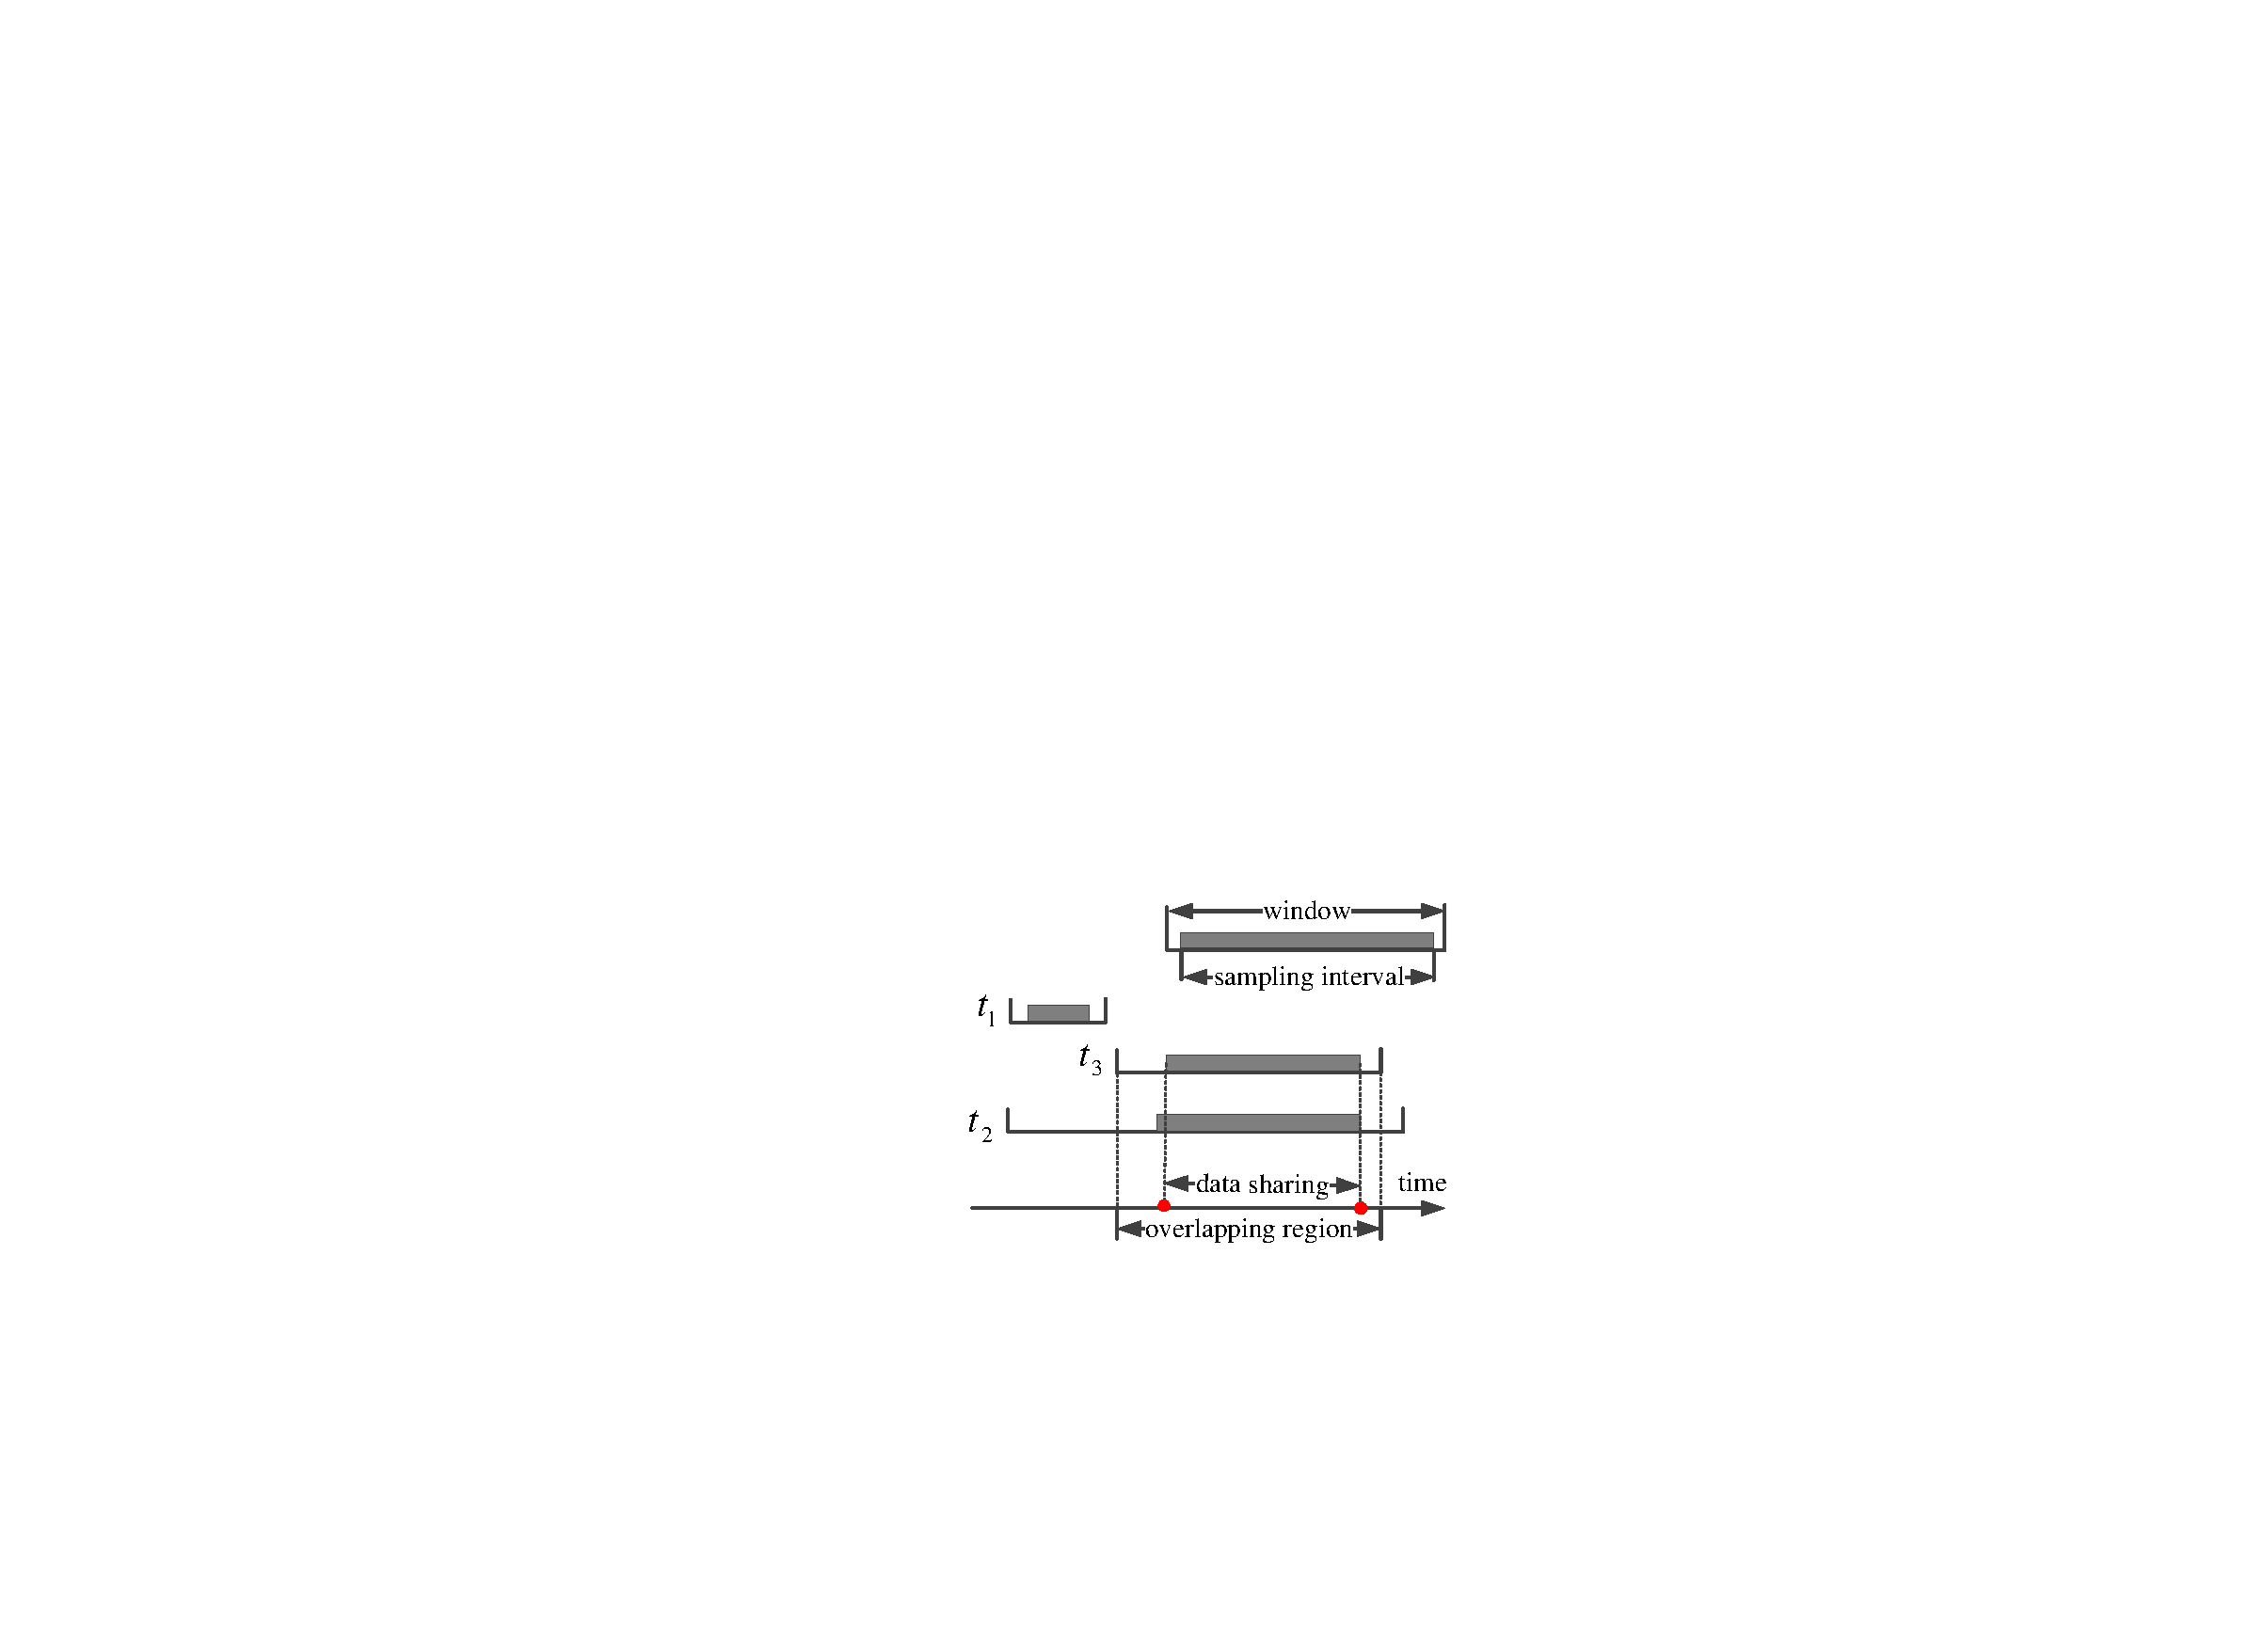
\includegraphics[width=0.45\columnwidth]{Figures/figure_introduction_scheduling}\label{figure_introduction_scheduling}}
%\subfigure[Task allocation]{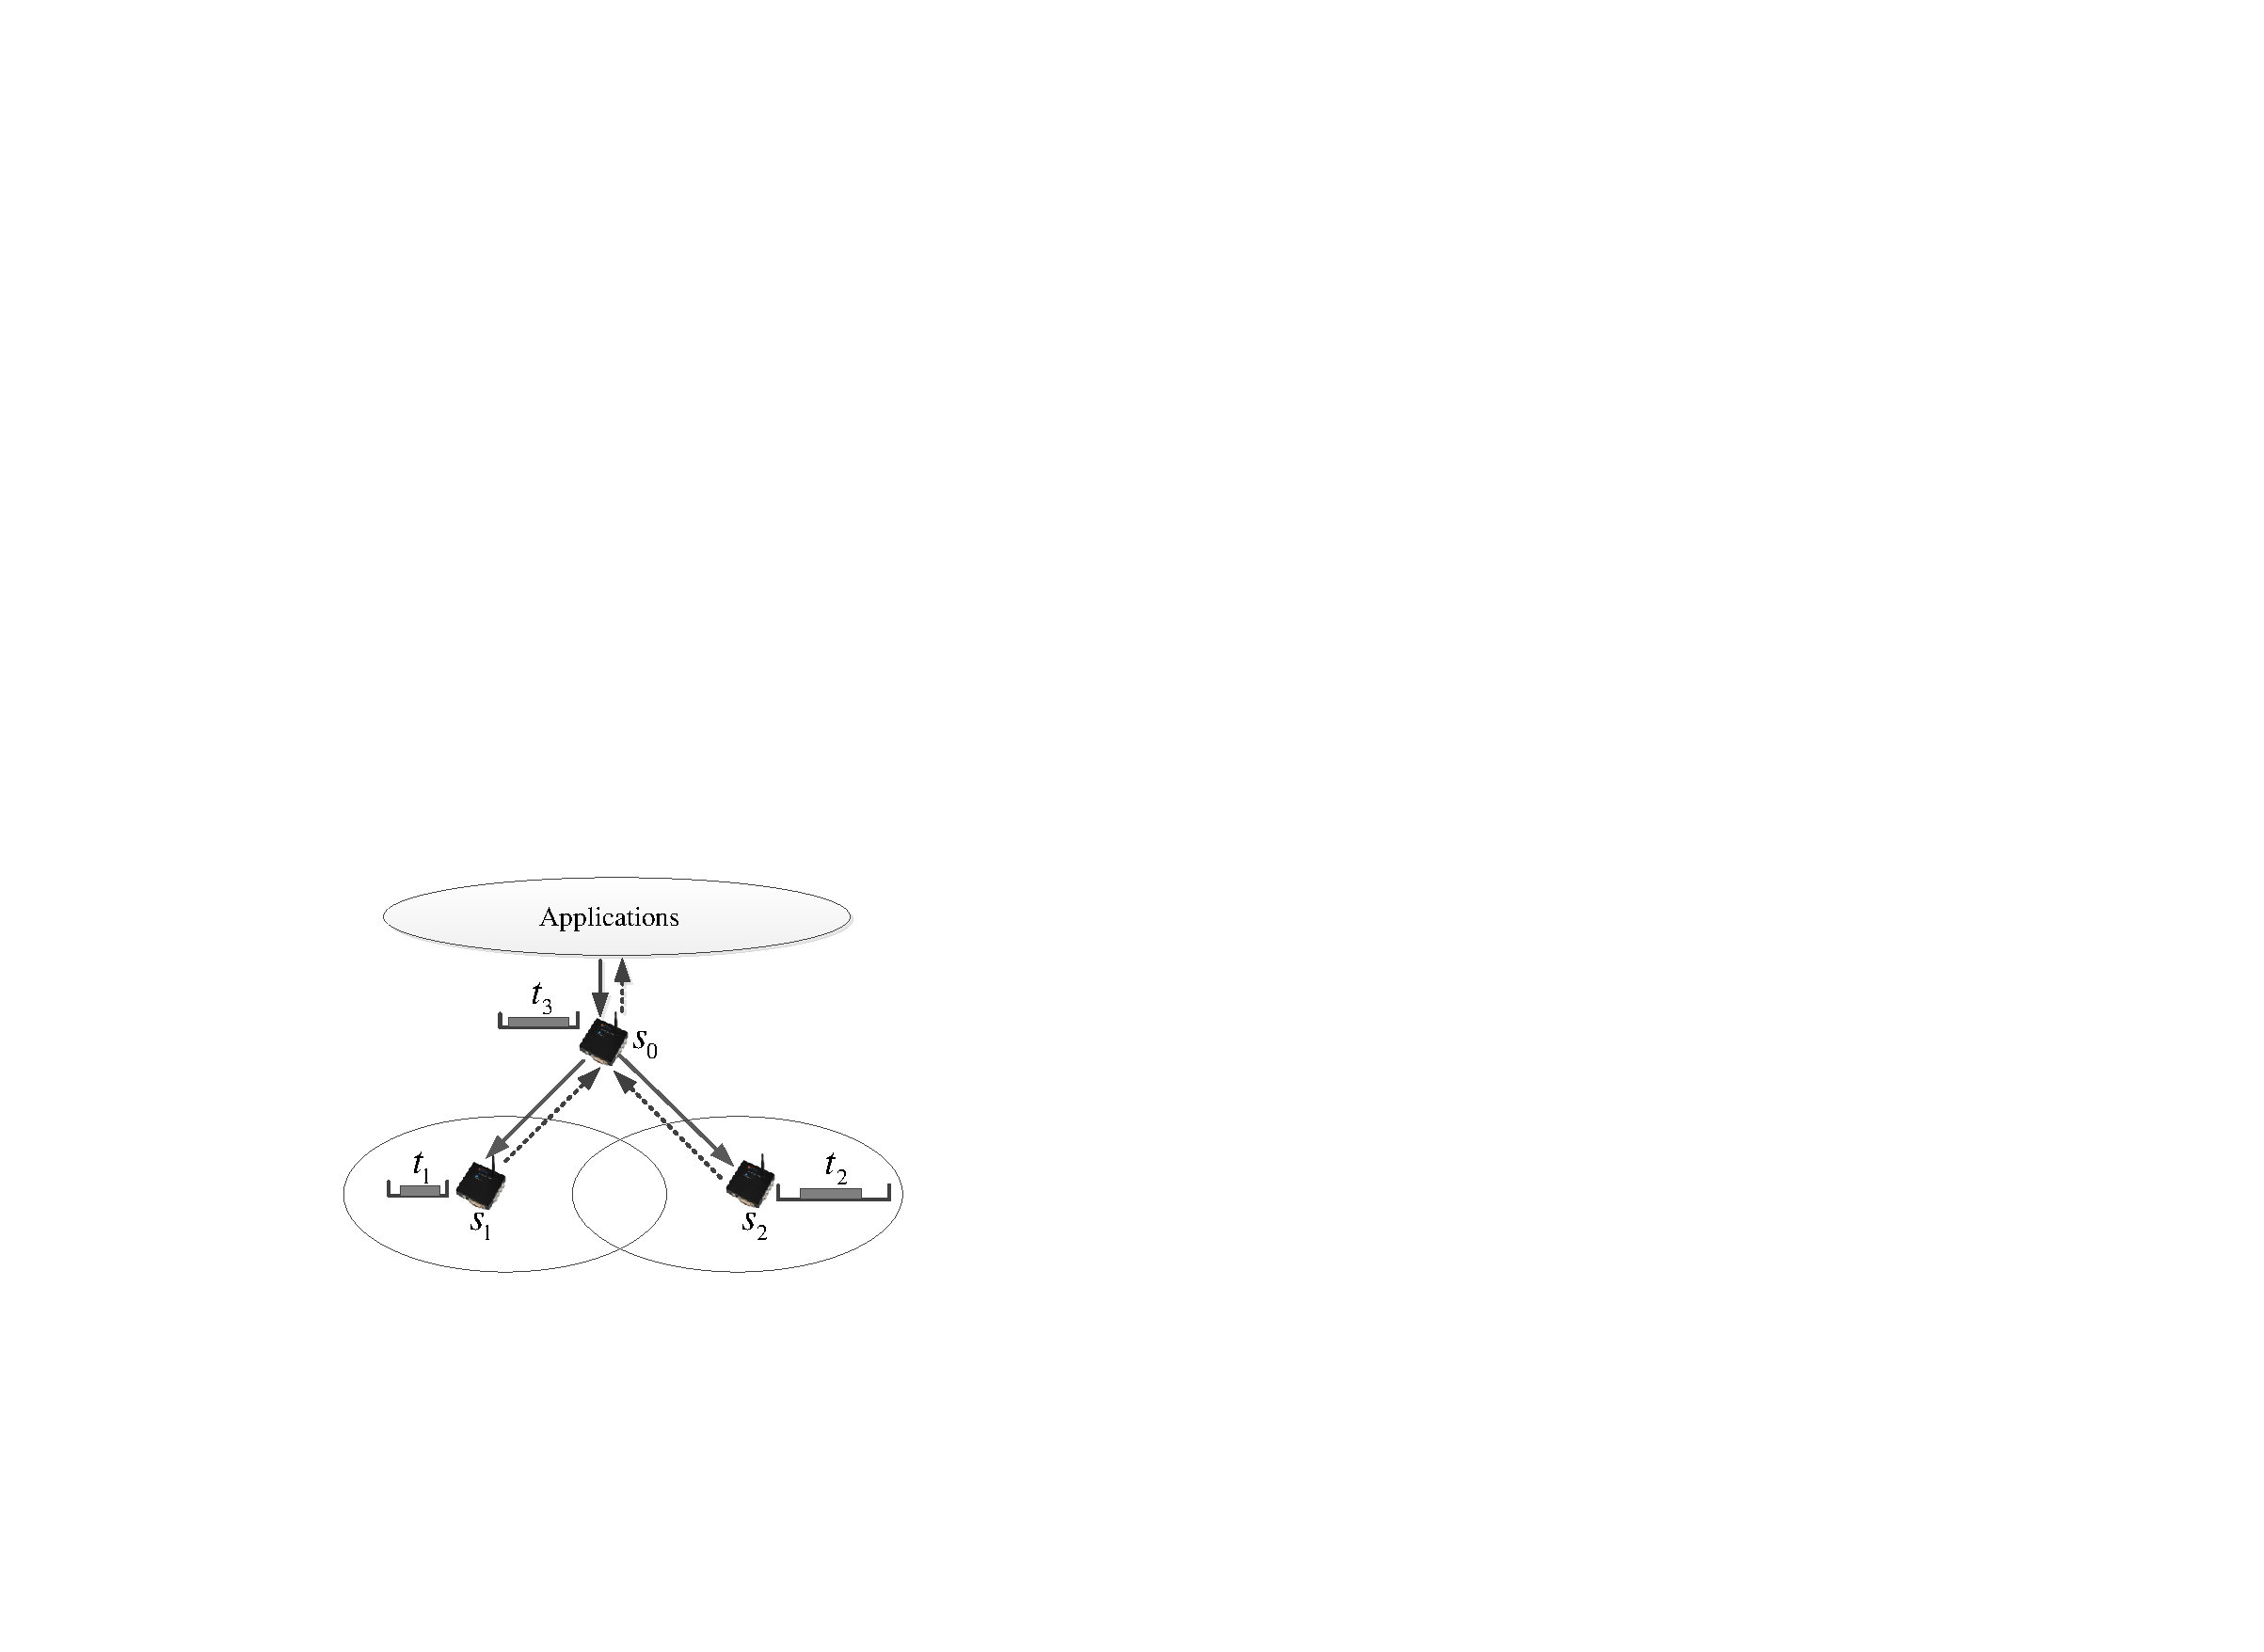
\includegraphics[width=0.5\columnwidth]{Figures/figure_introduction_allocation}\label{figure_introduction_allocation}}
%\caption{The illustrative examples for the scheduling of \emph{sampling interval} in the left panel and the allocation of tasks in the right panel.} \label{figure_introduction}
%\end{figure}


Recent literature has made some contributions on maximizing the data sharing amongst interval sampling tasks \cite{2013fang}. Fang et al. propose an effective task scheduling method for a task set which runs on a single node \cite{2013fang}. However, the scheduling strategy designed for a single node cannot be immediately extended to entire WSNs. It is thought to be invalid for entire WSNs due to an improper plan of task allocation amongst multiple nodes. Generally, actual deployed WSNs are $k$-coverage and $r$-redundant networks (Section \ref{section_prelimenary_model}) which make a balance between the reliability of entire network and the quality of communication \cite{2005_coverage_problem}, \cite{2007_undergroundMonitoring}, \cite{2013_TPDS_coverage}. The proposed data sharing strategies in \cite{2013fang} are not suitable to such a situation where data sharing amongst multiple sampling tasks becomes extremely complicated. The reason is that the methods proposed in \cite{2013fang} only consider how to maximize data sharing after sampling tasks have been allocated to sensor nodes, which ignore the potential gains of data sharing during task allocation. Since the strategy of task allocation has a great impact on the possible data sharing during task scheduling, only can the optimization of task scheduling be not enough. Instead, the allocation and scheduling of tasks should be taken into consideration together in order to maximize the data sharing for entire WSNs. For example, as illustrated in Fig. \ref{figure_introduction_allocation}, the sink node $s_0$ accepts sampling tasks $t_1$, $t_2$ and $t_3$ from applications and then allocates them to other nodes, namely, $s_1$ and $s_2$. When $s_1$ and $s_2$ complete the tasks, all the sampled  data will be sent to the sink node $s_0$ and then consumed by the applications. If the tasks $t_1$ and $t_2$ have been allocated to the nodes $s_1$ and $s_2$, respectively, then the task $t_3$, as illustrated in Fig. \ref{figure_introduction_scheduling}, should be allocated to $s_2$ due to more data sharing, that is, the overlapping time region between $t_2$ and $t_3$.  The scheduling method proposed by \cite{2013fang}, however, is not an effective solution for the entire network due to ignoring the overlap time region between tasks.

In a practical system, each node is usually assigned with more than one task during its life cycle. The conventional sampling strategy, i.e., First-In-First-Service (FIFS), does not help much to use data sharing amongst multiple sampling tasks, due to ignoring the overlap among sampling tasks. In fact, as illustrated in Fig. \ref{figure_introduction_scheduling}, the sampling intervals can be adjusted in the time windows to increase the overlap and lead to more data sharing. To be specific, it is the adjusting these intervals to achieve the minimal amount of sampled data that faces two challenging issues as follows.

\begin{itemize}
\item{\bf{Task allocation:}} As demonstrated in Fig. \ref{figure_introduction_allocation}, three sensor nodes $s_0$, $s_1$ and $s_2$ in WSN are considered. Here, $s_0$ is the sink node which is responsible for  allocating sampling tasks to $s_1$ and $s_2$. A data-intensive application injects three sampling tasks  $t_1$, $t_2$ and $t_3$ into the network, as shown in Fig. \ref{figure_introduction_scheduling}. If $t_1$ and $t_2$ have been allocated to $s_1$ and $s_2$, respectively, $t_3$ should be allocated to $s_2$. The reason is that the time window of $t_3$ and that of $t_2$ are overlapped. Therefore,  sampling interval of $t_3$ and that of $t_2$ can be adjusted to achieve to maximal data sharing. The problem of task allocation is NP complete (See Theorem \ref{theorem_problem_allocation} in Section \ref{section_preliminary_problem}). Consider that extensive data-intensive applications generate a large set of sampling tasks. It is extremely difficult to allocate these tasks in order to maximize data sharing with a resource-constrained sensor node.

\item{\bf{Task scheduling:}} As illustrated in Fig. \ref{figure_introduction_scheduling}, three sampling tasks $t_1$, $t_2$ and $t_3$ which have been allocated to a sensor node. Since the time window of $t_2$ and $t_3$ have the maximal overlapping time region. Sampling intervals of $t_2$ and $t_3$ can be adjusted to achieve the maximal data sharing when data is sampled in the overlapping time region. The problem of scheduling sampling interval is NP complete (See Lemma \ref{lemma_scheduling} in Section \ref{section_preliminary_problem}). Consider that a sensor node may be allocated numerous sampling tasks in a monitoring system. It is very difficult to solve the scheduling problem in polynomial time with a resource-constrained sensor node.
\end{itemize}

In this paper, we aim at maximizing of  the interval sampling data bearing the view of the entire WSN, rather than a single sensor node. The optimization problem is non-convex, and it is impossible to find an optimal solution for the resource-limited sensor nodes (Section \ref{section_preliminary_problem}). Therefore, we provide an effective solution by two steps, i.e., task scheduling and task allocation. Our basic idea, according to Fig. \ref{figure_introduction}, is to allocate and schedule a task set by utilizing the overlap amongst multiple sampling tasks. To address the above issues, we first formulate the optimal problem in a $k$-coverage and $r$-redundant WSN. We then propose a 2-factor approximation scheduling method which aims to minimize the amount of sampled data for a sampling task set. Furthermore, a 2-factor approximation task allocation method is proposed to reduce the amount of unnecessary sampled  data when tasks are allocated. To evaluate the correctness and the performance of our methods, we first conduct real implementations on a testbed containing  $5\mathrm{\times}10$ arrays of wireless sensor nodes. Simulations are further conducted in the widely-used simulation tool, i.e., TOSSIM. The evaluation results indicate that our methods significantly
reduce the amount of sampled data and energy consumption and therefore improve the bandwidth and reliability of wireless communication in WSNs.

The rest of this paper is organized as follows. Section \ref{section_related_work} summarizes related work. Section
\ref{section_prelimenary} defines the basic models of the network and sampling task, and then formalizes the optimization problem.  Section \ref{section_schedule} proposes a 2-factor approximation task  scheduling method for a sampling task set.  Section \ref{section_allocation} focuses on the task allocation problem and proposes a 2-factor approximation allocation method. Section \ref{section_evaluation} evaluates the correctness and performance of our proposals with extensive experiments. Finally, Section \ref{discussion} further discusses our solution and Section \ref{conclusion} concludes this paper.

\section{Related Work}
\label{section_related_work}
\subsection{Energy-aware task allocation and scheduling mechanisms in WSNs}
Xu et al. propose an energy-balanced method of task allocation which implements the maximal energy dissipation amongst all sensor nodes \cite{2010_near_optimal_mobihoc}. The tasks are executed during the beginning of each epoch and must be completed before the end of the epoch. That is, the epoch of a task is similar to the time window of the task model in the paper. It is noted that tasks in \cite{2010_near_optimal_mobihoc} is communication tasks, not the sampling tasks. The difference results in that the proposed method in \cite{2010_near_optimal_mobihoc} does not suit to our problem. Additionally, the solution for solving an integer linear programming problem in \cite{2010_near_optimal_mobihoc} costs much time. Packets in \cite{2006_time_optimum_mass} own the same properties of a sampling task we discuss in the paper. The release time and the deadline of a packet represent the beginning time and the end time, respectively. The difference is that a packet reports one unit of data, rather than the data which is sampled over a time interval continuously. Thus, the methods in \cite{2006_time_optimum_mass} work well for the discrete point sampling tasks, not the interval sampling tasks.

The most related work to ours are \cite{2010task_optimization} and \cite{2013fang}. Tavakoli et al. present an approach for task scheduling on a sensor node to minimize the network communication overhead \cite{2010task_optimization}. A task in \cite{2010task_optimization} is a discrete point sampling task and requires to be performed via once data sampling during its time window. Therefore, the method proposed in \cite{2010task_optimization} does not suit to our problem.  Fang et al.  propose an effective sampling approach for interval sampling tasks on a single sensor node \cite{2013fang}. The $2$-factor approximation algorithm in \cite{2013fang} is the state-of-the-art method to maximize the data sharing amongst tasks on a single node. Unfortunately, there are two weak points in \cite{2013fang}. First, the proposed scheduling method schedules sampling tasks in the ascending order of the end time of tasks. As a result, such scheduling strategy neglects data sharing between overlapping tasks. Moreover, Fang et al. assume that all tasks have the same length of sampling interval, which is too ideal and not practical. By contrast, we observe that multiple tasks may be overlapping, and thereby data sharing exists. Our solution exploits this feature and thus achieves better performance on maximizing the data sharing than the scheduling method in \cite{2013fang}. Second, the solution in \cite{2013fang} only focuses on task scheduling on a single sensor node, and does not consider the process of task allocation in a WSN. As we have discussed, the performance of algorithms of task scheduling is sensitive to the strategy of task allocation. Only does optimizing the process of the former not achieve the final optimization for a deployed system. Our solution is more general and practical because of jointly optimizing the process of task allocation and that of scheduling sampling interval.

\subsection{Multi-query optimization in  WSNs}
Recently, a WSN is treated as a database providing a good logical abstraction for sensor data management. The aim of multi-query optimization in such a database system studies how to efficiently process queries \cite{2007_two_tier_icdcs}, \cite{2005_multi_query}. Xiang et al. adopt a two-tier multiple query optimization scheme to minimize the average transmission time in WSNs \cite{2007_two_tier_icdcs}. The first-tier optimization is a cost-based approach which schedules queries as a whole and eliminates duplicate data requests from original queries. Since it is not the optimization of the volume of sampled data, such an approach cannot be used for our problem. Moreover, the second-tier optimization acquires and transmits sampled data by using the broadcast nature of the radio channel. Our solution aims to provide a general solution for maximizing data sharing amongst sampling tasks. The details of wireless communication is not involved in our method.  Trigoni et al. consider multi-query optimization by using aggregation operations such as \emph{sum} and \emph{avg} to achieve the optimal communication cost \cite{2005_multi_query}; while our method mainly concerns minimal energy consumption by reducing redundant sampled data.

\subsection{Compression techniques based data collection}
Compression-based data collection significantly reduces redundancy of sampled data for a sensor node \cite{2003_PINCO,2002_distributed_compression}. Arici et al. propose an in-network compression scheme (PINCO) for a densely deployed WSN. PINCO compresses raw data by reducing redundancy existing in sensor readings in spatial, temporal and spatial-temporal domains \cite{2003_PINCO}. Unfortunately, PINCO trades higher latency for lower energy consumption due to the process of data compression. Such weakness limits its effectiveness in some latency aware applications. By contrast, our solution does not cost time to analyze and compress the raw data. Moreover, PINCO only considers the single-valued data (humidity, temperature, etc.).  Since single-valued data is produced by the discrete point sampling tasks, methods in \cite{2003_PINCO} cannot be used to solve our problem directly. Using fast error-correcting coding algorithms, Pradban et al. present a framework on the distributed souring coding technique to reduce data redundancy \cite{2002_distributed_compression}. However, method in \cite{2002_distributed_compression} requires to get known of the sensor correlation structure. It is impossible for a randomly deployed system such as a battlefield monitoring system.


\section{Preliminaries}
\label{section_prelimenary}
Before we further discuss the optimization problem of interval sampling for a task set in WSNs, the basic task and the network models used in this paper are formalized. Based on these models, we first define the optimization problem for a task set in WSNs by using the idea of interval data sharing. We then define a metric for measuring the data sharing amongst sampling tasks, which will be used to design the effective allocation and scheduling methods for a task set.
\subsection{Task and network models}
\label{section_prelimenary_model}
The task model and the WSN model are formalized by Definition \ref{task_model} and Definition \ref{system_model}, respectively.

\begin{figure}[t]
\centering
\subfigure[Task model]{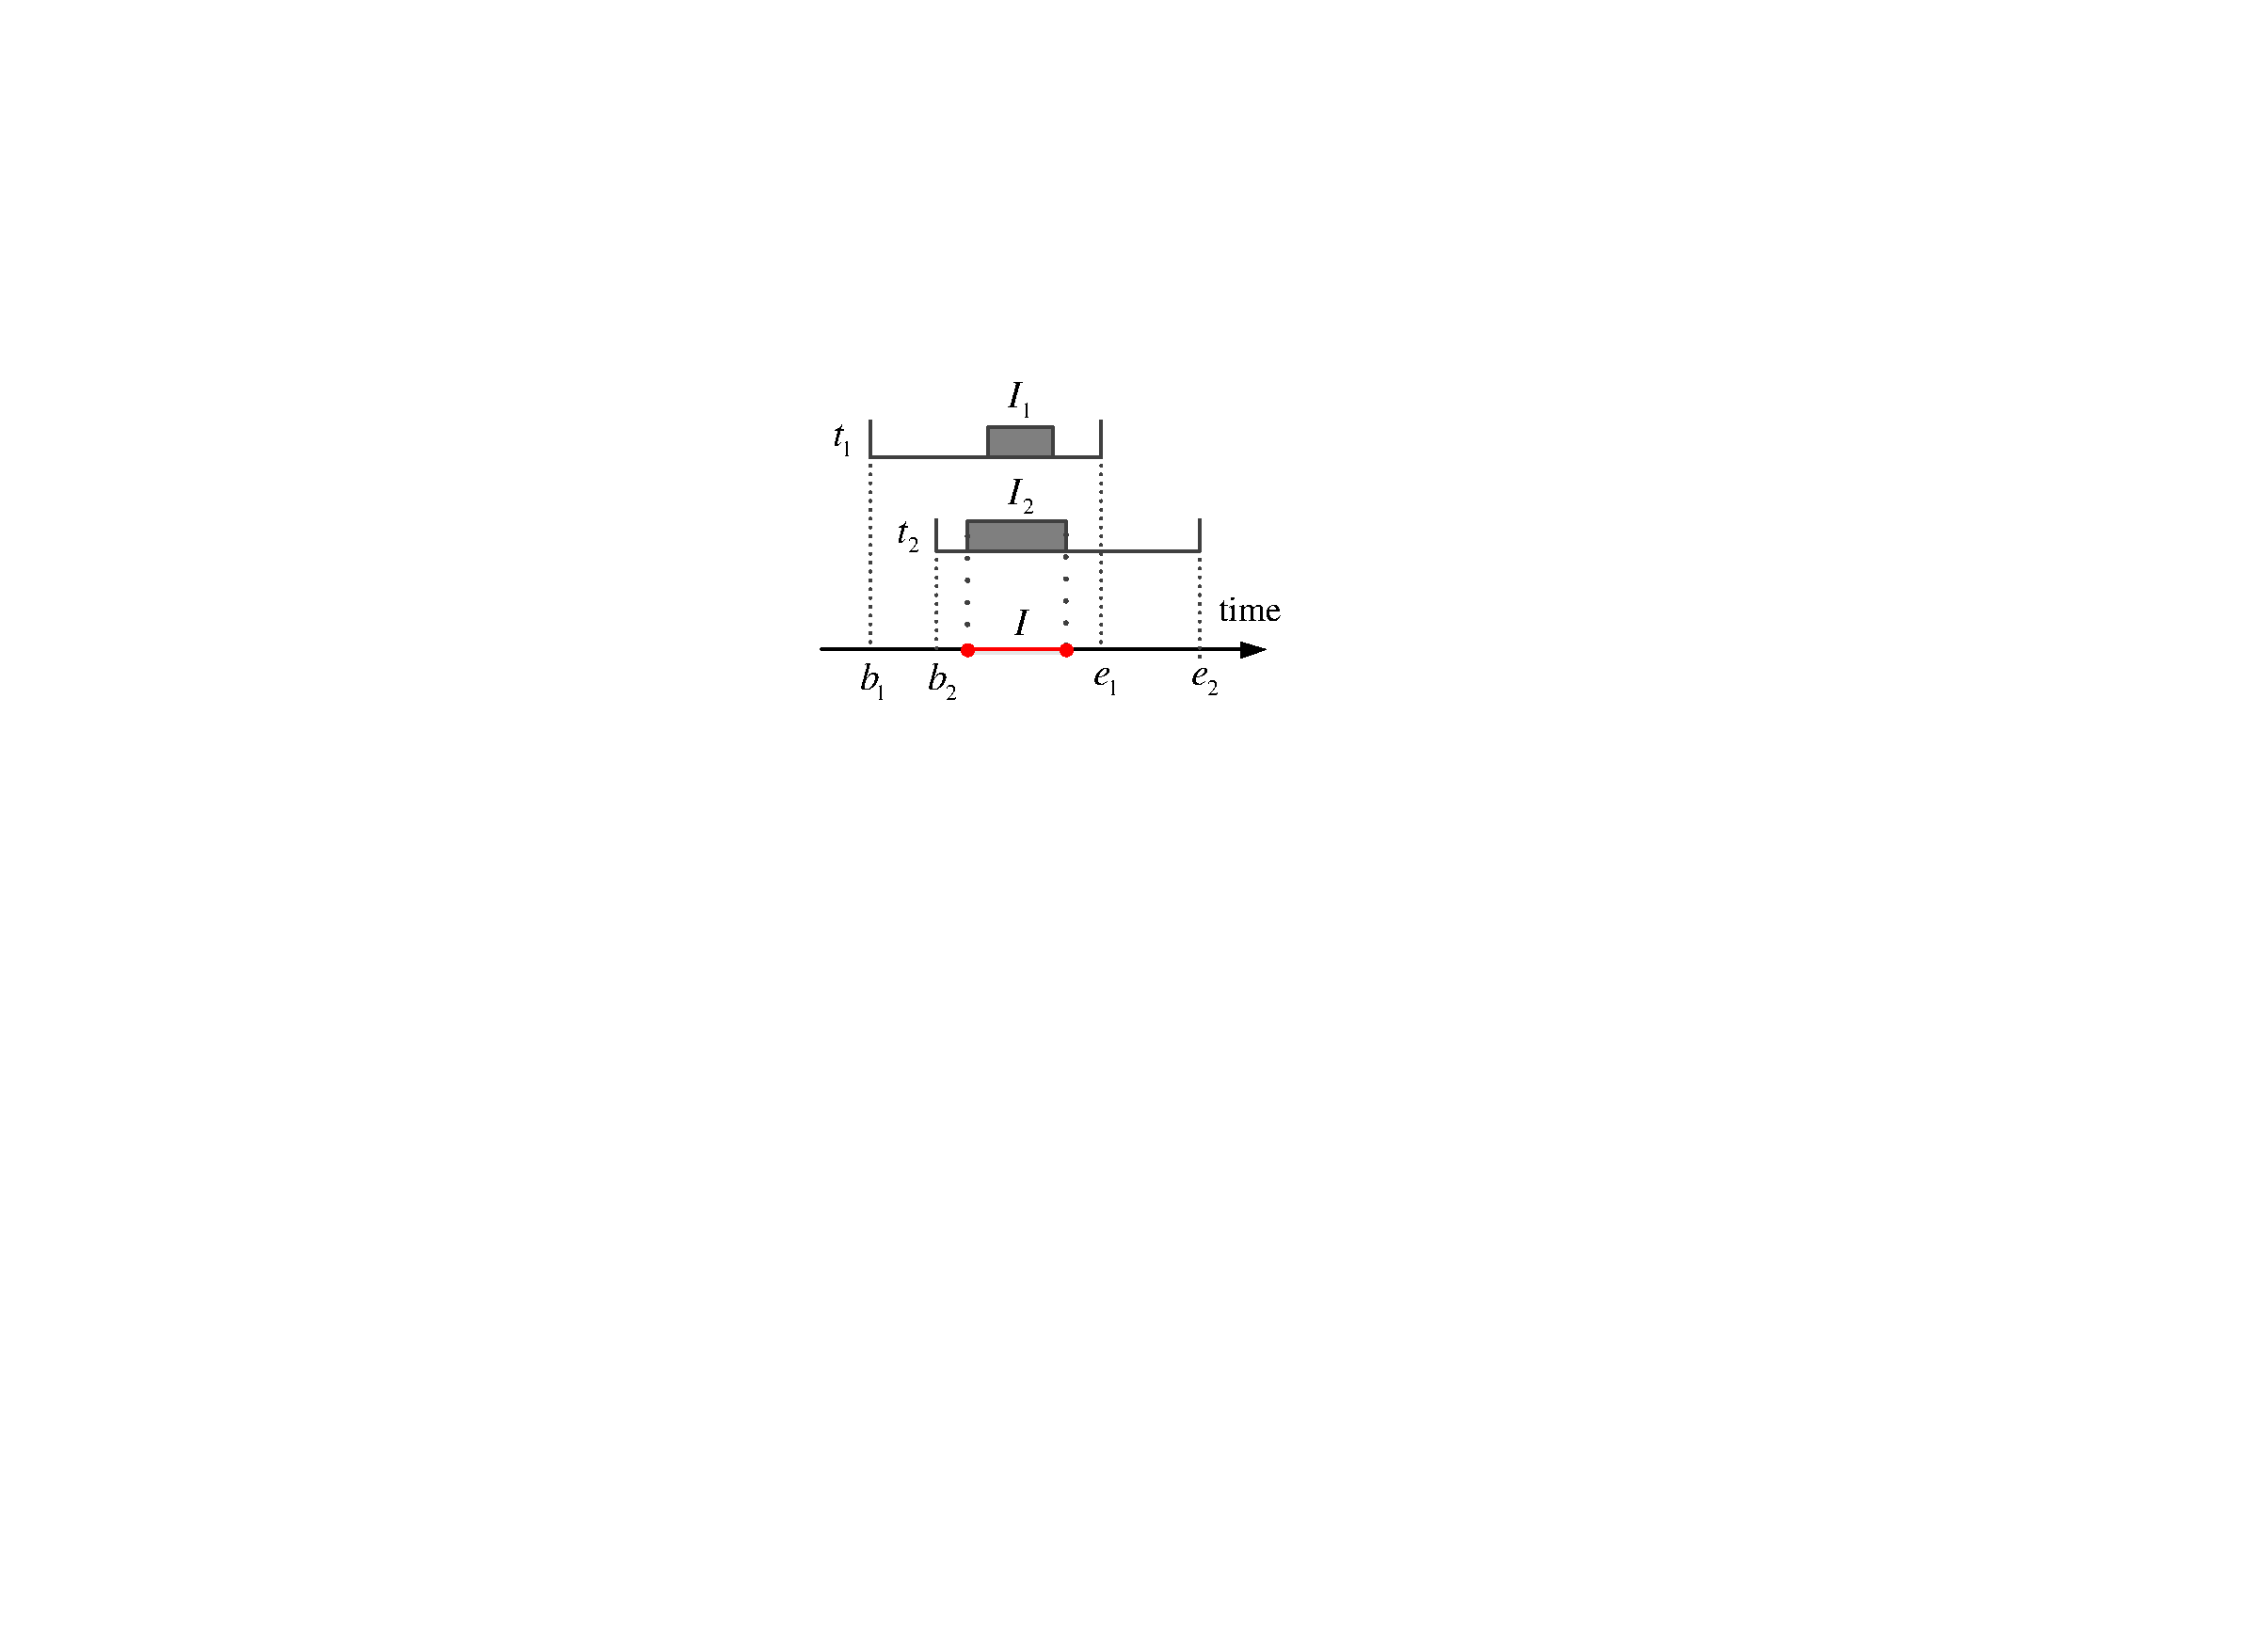
\includegraphics[width=0.3\columnwidth]{Figures/figure_overview_task_model}\label{figure_task_model}}
\hspace{6pt}
\subfigure[Network model]{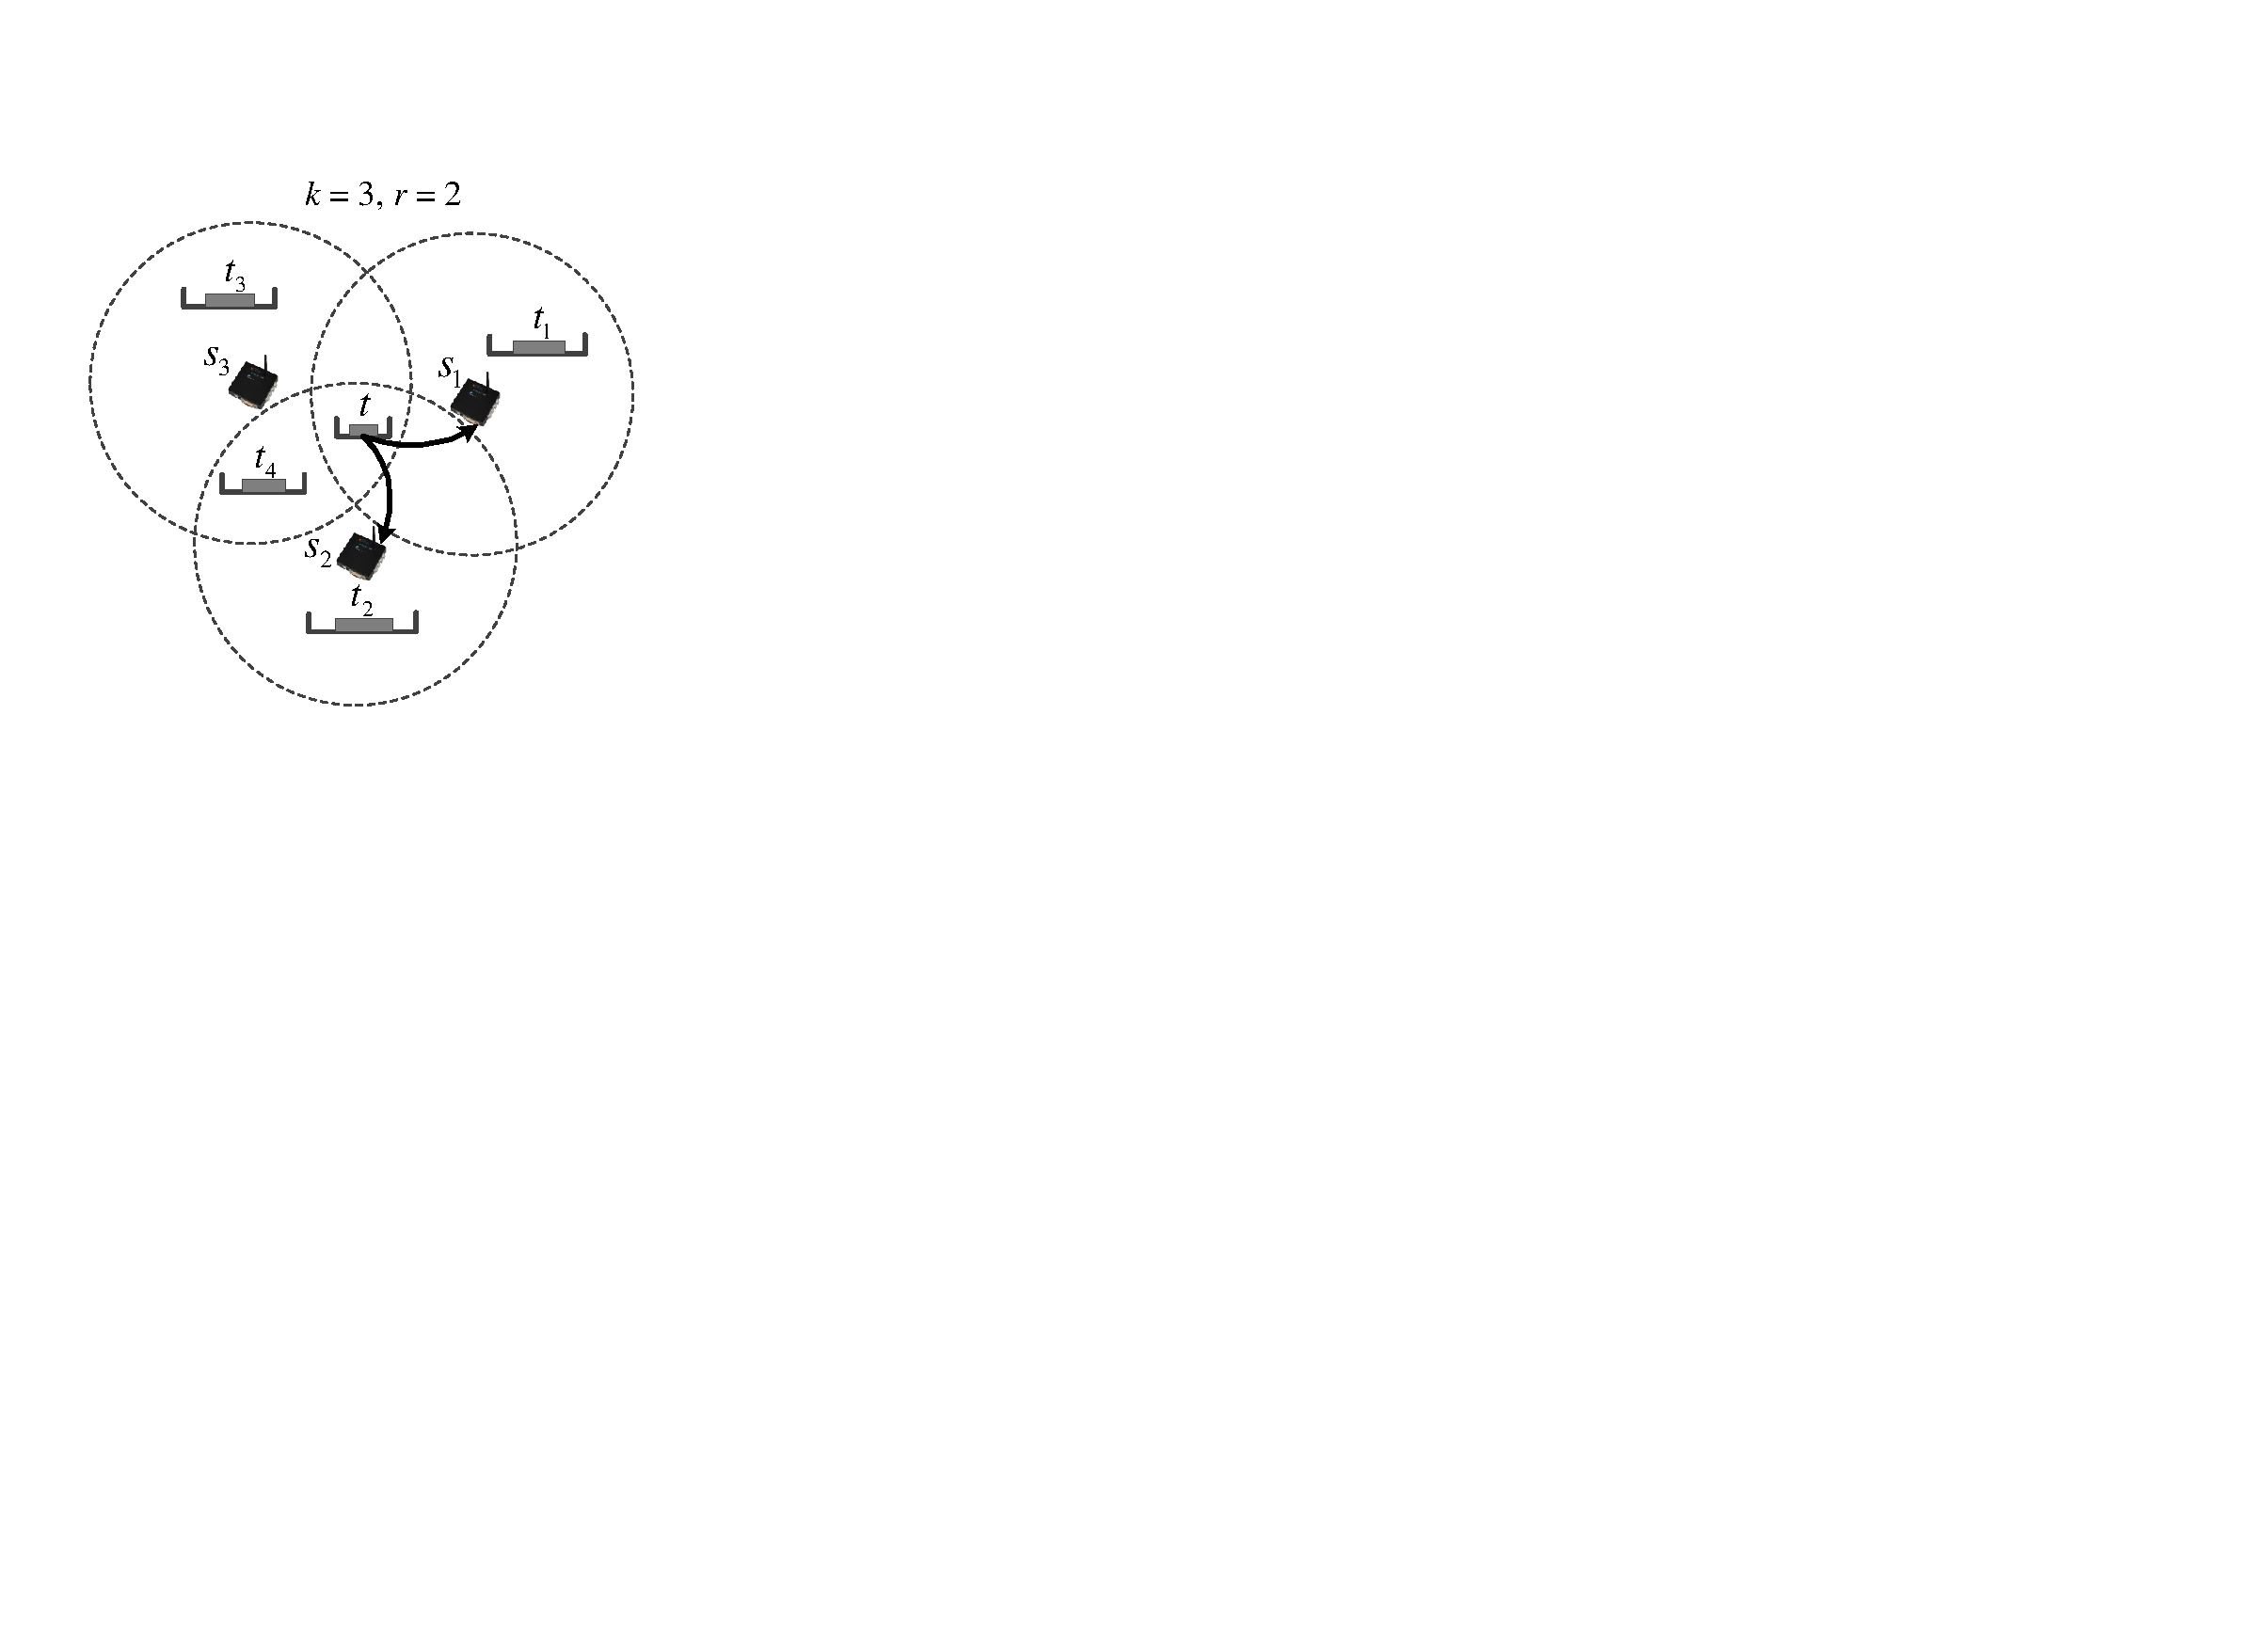
\includegraphics[width=0.33\columnwidth]{Figures/figure_overview_network_model}\label{figure_network_model}}
\caption{The task and network models for the interval data sampling.}
\label{figure_overview}
\end{figure}


\begin{definition}[Interval sampling task]
Given a task $t$, it can be defined as a triple $\mathrm{<}b,e,l\mathrm{>}$ where $b$, $e$ and $l$ represents the begin time, the end time and the interval length of the task, respectively. Its time window is denoted by $[b,\; e]$, and the sampling interval can flexibly move in the time window. \label{task_model}
\end{definition}

In the view of a single sensor node, when a task is overlapping with other tasks, they can be scheduled to share the sampled data in the overlapping region to reduce the amount of sampled data. As illustrated in Fig. \ref{figure_task_model}, there are two overlapping tasks $t_1\mathrm{=<}b_1,e_1,l_1\mathrm{>}$ and $t_2\mathrm{=<}b_2,e_2,l_2\mathrm{>}$. Here, $b_i$, $e_i$ and $l_i$ are the begin time, the end time and the corresponding sampling interval of the task $t_i$ ($i$ may be valued 1 or 2).  The sampling interval $I$ satisfies the requirements of two tasks, but its interval length  is smaller than the sum of intervals $I_1$ and $I_2$ due to the utilization of data sharing between $t_1$ and $t_2$. For a single sensor node, the best scheduling solution is to minimize the amount of sampled data, decreases energy consumption, and prolongs its lifetime. However, the scheduling problem is NP complete (Lemma \ref{lemma_scheduling} in Section \ref{section_preliminary_problem}). We first discuss the scheduling problem and give a 2-factor approximation scheduling algorithm in Section \ref{section_schedule}.

\begin{definition}[$k$-coverage and $r$-redundant network]
Given a wireless sensor network $N$, it can be represented as $N\mathrm{=(}S,T,k,r\mathrm{)}$. Here, $S$ and $T$ represent the node set and the task set of the WSN, respectively. The notation $k$ means a task in the network can be detected by $k$ sensor nodes, but only $r$ out of them are identified to execute the task. $k$ is determined when a wireless sensor network is deployed. $r$ is set by the  requirement of communication quality or applications, and is universal to all the sampling tasks.
\label{system_model}
\end{definition}

As illustrated in Fig. \ref{figure_network_model}, the wireless sensor network consists of three sensor node $s_1$, $s_2$, and $s_3$. Each of them has a sensing range (indicated by the dotted circle). The  tasks $t_1$, $t_2$, $t_3$ and $t_4$ have been allocated to a sensor node if which can be detected by the node. The task $t$ is detected by three sensor nodes in WSNs, i.e., $k \mathrm{=} 3$. In fact, to guarantee the requirement of the communication quality and that of applications, $t$ is eventually assigned to two sensor nodes, i.e., $r\mathrm{=}2$. Thus, the allocation problem exists and will be discussed in Section \ref{section_allocation}.


We aim to minimize the amount of sampled data for the sampling tasks bearing the view of WSNs. The optimization problem contains two subproblems: allocating tasks amongst multiple candidate sensor nodes, and scheduling tasks for a sampling task set. Even though the optimization problem is extremely difficult, it is valuable and meaningful. A good allocation solution will reduce much unnecessary sampled data, which benefits the quality of communication so as to relieve delay and congestion of the entire network.

%\begin{table}[b]
%\small
%\centering
%\caption{Symbols list}
%\begin{tabular}{|c|l|c|l|}
%\hline
%    \multicolumn{1}{|c|}{Symbol}& \multicolumn{1}{c|}{Notation}& \multicolumn{1}{c|}{Symbol}& \multicolumn{1}{c|}{Notation}\\ \hline
%    $t$& a task& $s$& a sensor node\\ \hline
%    $T$& a task set& $S$& a sensor node set\\ \hline
%    $n$& the cardinality of $T$&$b$& the begin time\\ \hline
%    $m$& the cardinality of $S$&$e$& the end time\\ \hline
%    $\Phi$& the interval set&$\mathrm{<}b,e,l\mathrm{>}$&a triple for a task\\ \hline
%    $Q$&  a quad list& $q$& a quad\\ \hline
%    $x_{ij}$& an indicator variable&$I$& an interval set\\ \hline
%     $l$& the interval length&  $d(t_i,t_j)$& the overlap value\\ \hline
%    $\delta$&\multicolumn{3}{l|}{the same interval length used in a compact model}\\ \hline
%    $\theta$&\multicolumn{3}{l|}{the number of compact tasks in a compact model}\\ \hline
%    ${C}(t_i,t_j)$&\multicolumn{3}{l|}{the new task after combination operation}\\ \hline
%    $k$& \multicolumn{3}{l|}{Any task can be executed by $k$ sensor nodes}\\ \hline
%    $r$& \multicolumn{3}{l|}{Any task is actually executed by $r$ sensor nodes}\\ \hline
%\end{tabular}
%\label{table_symbol}
%\end{table}

\begin{table}[!b]
\small
\centering
\tbl{Symbols list\label{table_symbol}}{
\begin{tabular}{|c|l|c|l|}
\hline
    \multicolumn{1}{|c|}{Symbol}& \multicolumn{1}{c|}{Meaning}& \multicolumn{1}{c|}{Symbol}& \multicolumn{1}{c|}{Meaning}\\ \hline
    $t$& a task& $n$& the cardinality of $T$\\ \hline
    $T$& a task set& $m$& the cardinality of $S$\\ \hline
    $s$& a sensor node&$b$& the begin time\\ \hline
    $S$& a sensor node set&$e$& the end time\\ \hline
    $I$& an interval&$\mid \cdot \mid$&cardinality of a set\\ \hline
    $\Phi$& an interval set&$x_{ij}$& an indicator variable\\ \hline
    $l$, $|I|$& the interval length&  $d(t_i,t_j)$& value of data sharing\\ \hline
    $\delta$&\multicolumn{3}{l|}{the same length of interval used in a compact model}\\ \hline
    $\varphi$&\multicolumn{3}{l|}{the number of compact tasks in a compact model}\\ \hline
    $t_{ij}$&\multicolumn{3}{l|}{a new task generated by combining $t_i$ and $t_j$}\\ \hline
    $k$& \multicolumn{3}{l|}{a task can be executed by $k$ sensor nodes}\\ \hline
    $r$& \multicolumn{3}{l|}{a task is actually performed by $r$ sensor nodes}\\ \hline
\end{tabular}}
\end{table}



\subsection{Interval data sharing based minimization of the amount of sampled data}
\label{section_preliminary_problem}
We define the optimization problem in this section. To ease the description, Table \ref{table_symbol} summarizes the frequently used symbols throughout the paper.



%\newtheorem{definition}{\bf{Definition}}
\begin{definition}
Given an interval $I$, and a $0\mathrm{-}1$ indicator variable $x_{ij}$. If the task $t_i$ is allocated to the node $s_j$, then $x_{ij}\mathrm{=}1$ else $x_{ij}\mathrm{=}0$. We define $x_{ij} \mathrm{\odot} I$ as follows:
\begin{equation}
x_{ij} \mathrm{\odot} I \mathrm{=} \left \{ \begin{array}
{r@{\quad:\quad}l}
I & x_{ij}\mathrm{=}1\\
\emptyset & x_{ij}\mathrm{=}0
\end{array} \right.
\end{equation}
\end{definition}

\begin{definition}
There are two intervals $I_1$ and $I_2$ with $I_1\mathrm{=[}u_1, v_1\mathrm{]}$ and $I_2\mathrm{=[}u_2, v_2\mathrm{]}$. As illustrated in Fig. \ref{figure_task_model}, $I_1$ and $I_2$ are overlapping when they have the common area on the time axis.
Assume $u\mathrm{=}\min\{u_1,u_2\}$ and $v \mathrm{=}\max\{v_1,v_2\}$, if $I_1$ and $I_2$ are overlapping,  we define a new interval $I$ as the union of $I_1$ and $I_2$, i.e., $I\mathrm{=}I_1 \mathrm{\uplus} I_2\mathrm{=}[u, v]$  and $|I| \mathrm{=} v\mathrm{-}u$. Here, `$\mathrm{\uplus}$' stands for the union operation of two intervals.
\end{definition}

\begin{definition}
Given a task set $T$ with $|T|\mathrm{=}n$, and a sensor node set $S$ with $|S|\mathrm{=}m$, each task $t_i$, $t_i\mathrm{\in}T$, is notated as a triple $\mathrm{<}b_i,e_i,l_i\mathrm{>}$. Since $r$ out of $k$ candidate sensor nodes are identified to perform the task $t_i$, the optimization problem is to find an allocation solution for $T$  so as to:

\begin{equation}
\min\sum^m_{j\mathrm{=}1}{|\biguplus_{i\mathrm{=}1}^n x_{ij} \odot I_i|}
\end{equation}
$s.t.:$\\
\begin{equation}
\left\{ \begin{array}{ll}
\sum^m_{j\mathrm{=}1} x_{ij}\mathrm{=}r,i\mathrm{=}1,...,n,1\mathrm{\le} r \mathrm{\le} k;\\
x_{ij}\mathrm{=}0  \; \; \mathrm{or} \;\; 1;\\
I_i\subseteq[b_i,e_i],i\mathrm{=}1,...,n;\\

\end{array} \right.
\end{equation}
\end{definition}

When $r\mathrm{=}k$, we should allocate each task into all candidate sensor nodes. The allocation solution is determined solely. Generally, when $0\mathrm{<}r\mathrm{<}k$, the object function is non-linear, which makes the optimization problem become very difficult. This kind of non-linear programming problem has no universal efficient solution. Several methods, including branch and bound techniques, require high computational complexity and are not applied to a wireless sensor node. Considering the limitation of computing and memory resources of sensor nodes, the non-linear programming problem becomes very hard to resolve. To be clarified clearly, the scheduling problem, minimizing the amount of sampled data for a task set, is marked as ``MIN-SA", and the allocation problem, minimizing the sum of sampled data for sampling tasks on multiple sensor nodes in WSNs, is marked as ``MIN-SSA".

\begin{figure}[t]
\centering
\subfigure[MAX-DHP in graph $G$.]{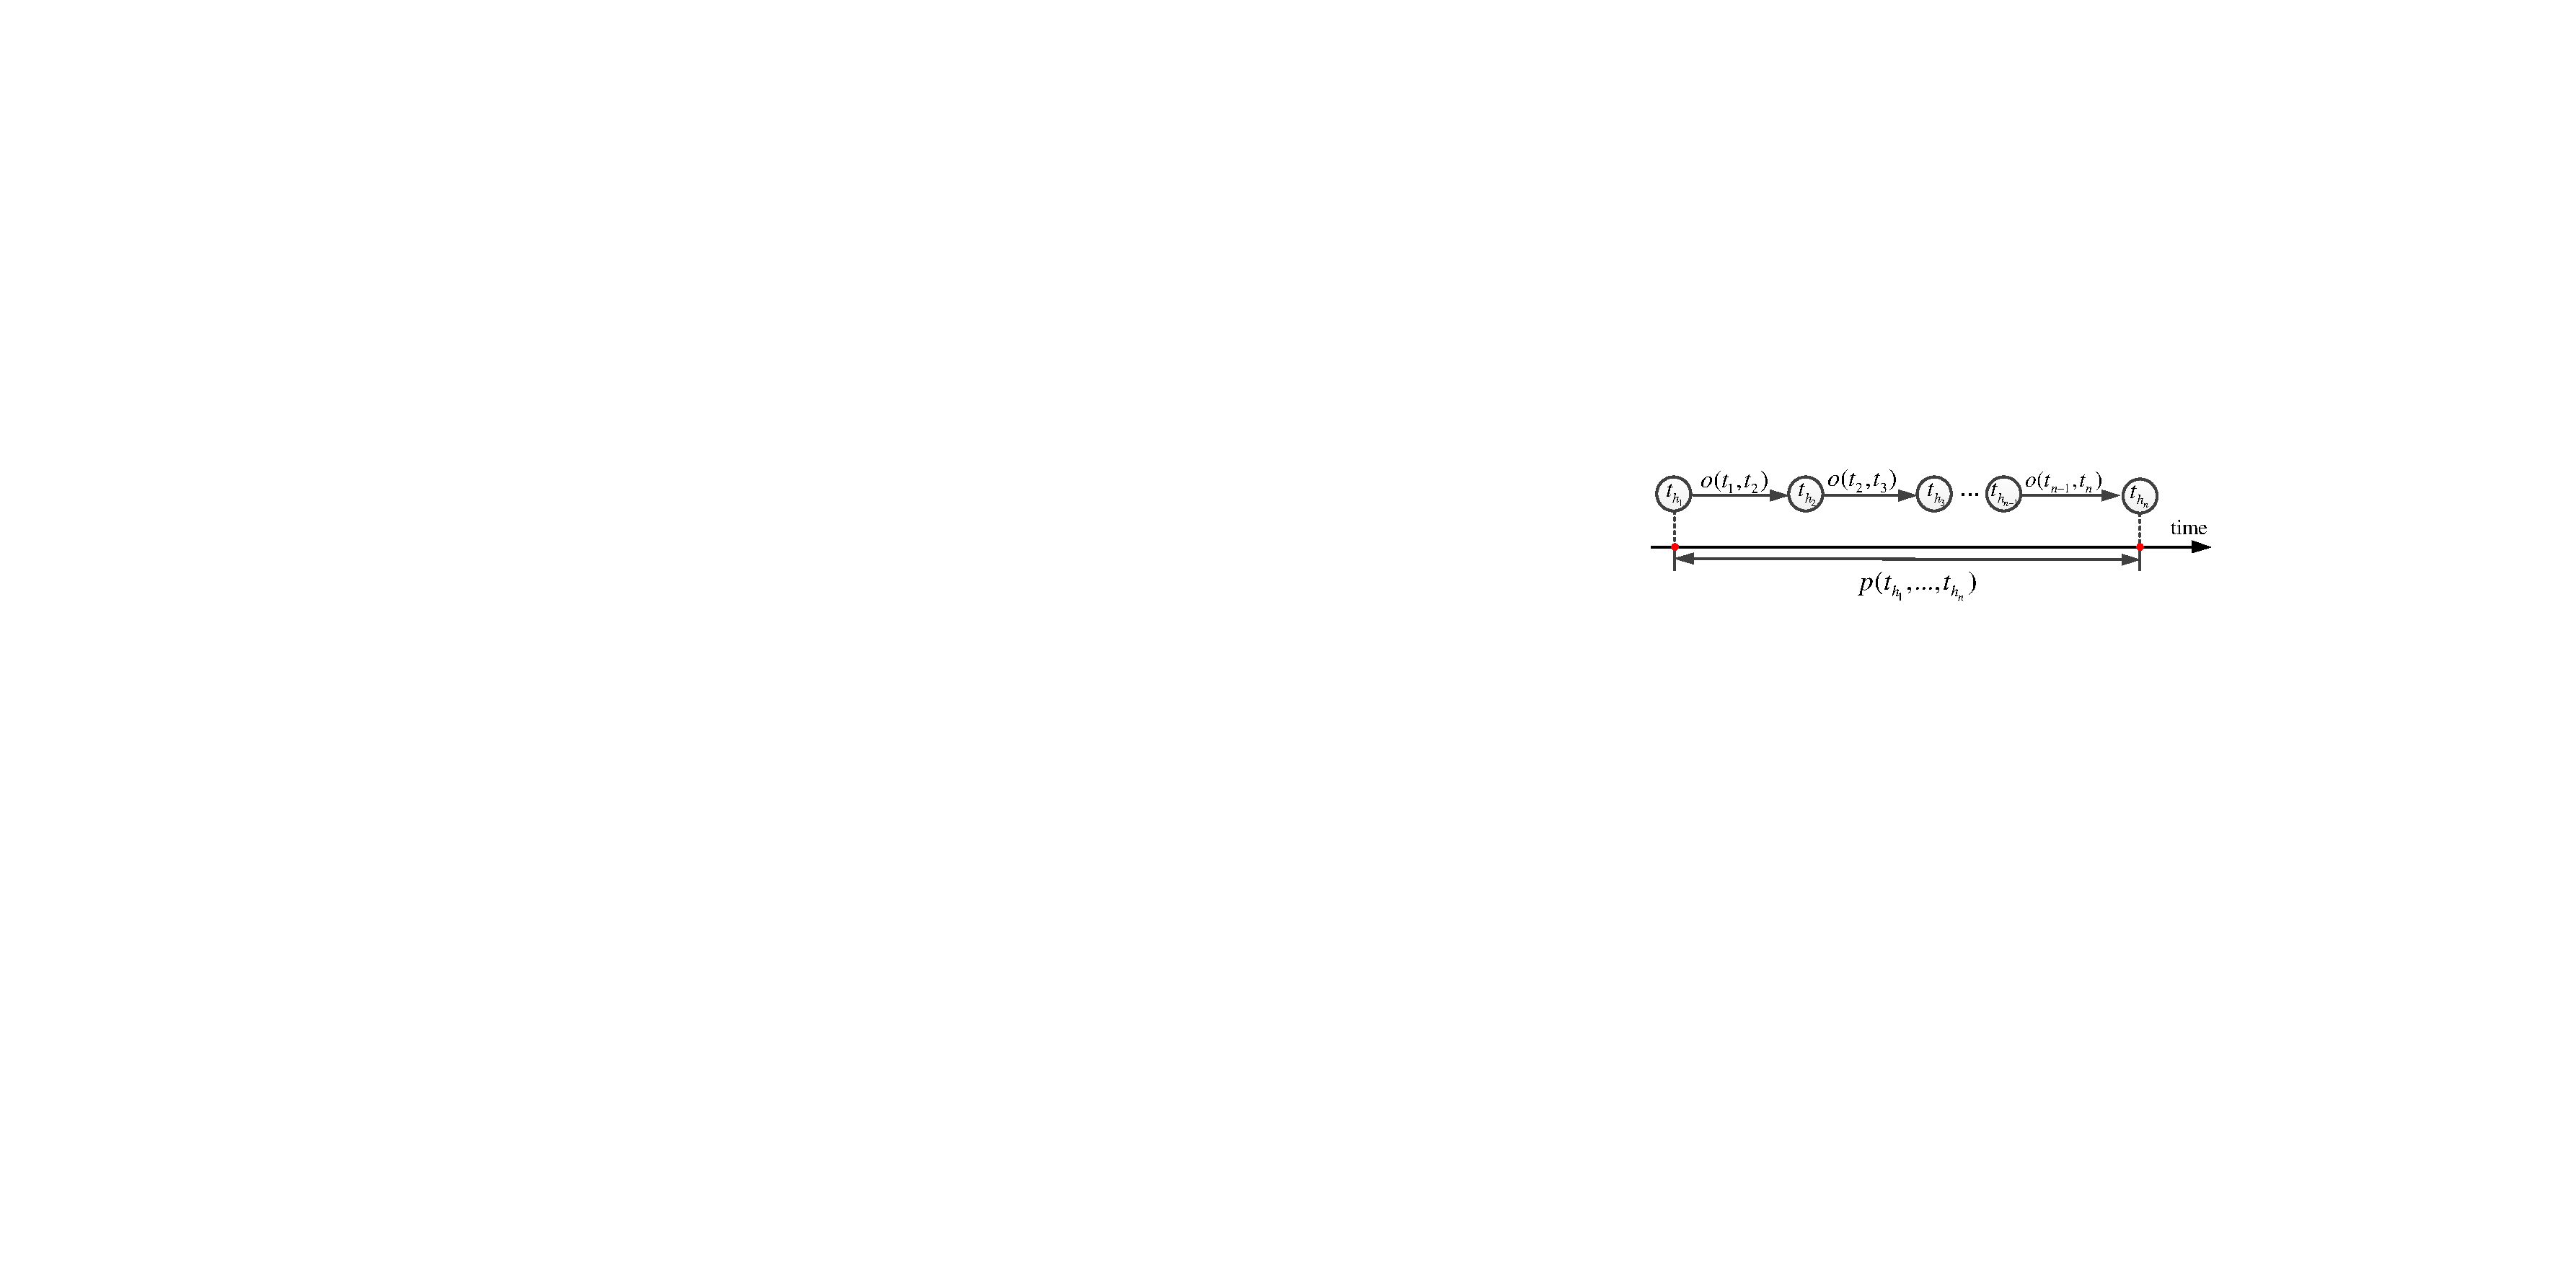
\includegraphics[width=0.52\columnwidth]{Figures/figure_proof_scheduling_1}\label{figure_proof_scheduling_1}}
%\hspace{p5pt}
\subfigure[MAX-DHP is reduced to the scheduling problem MIN-SA.]{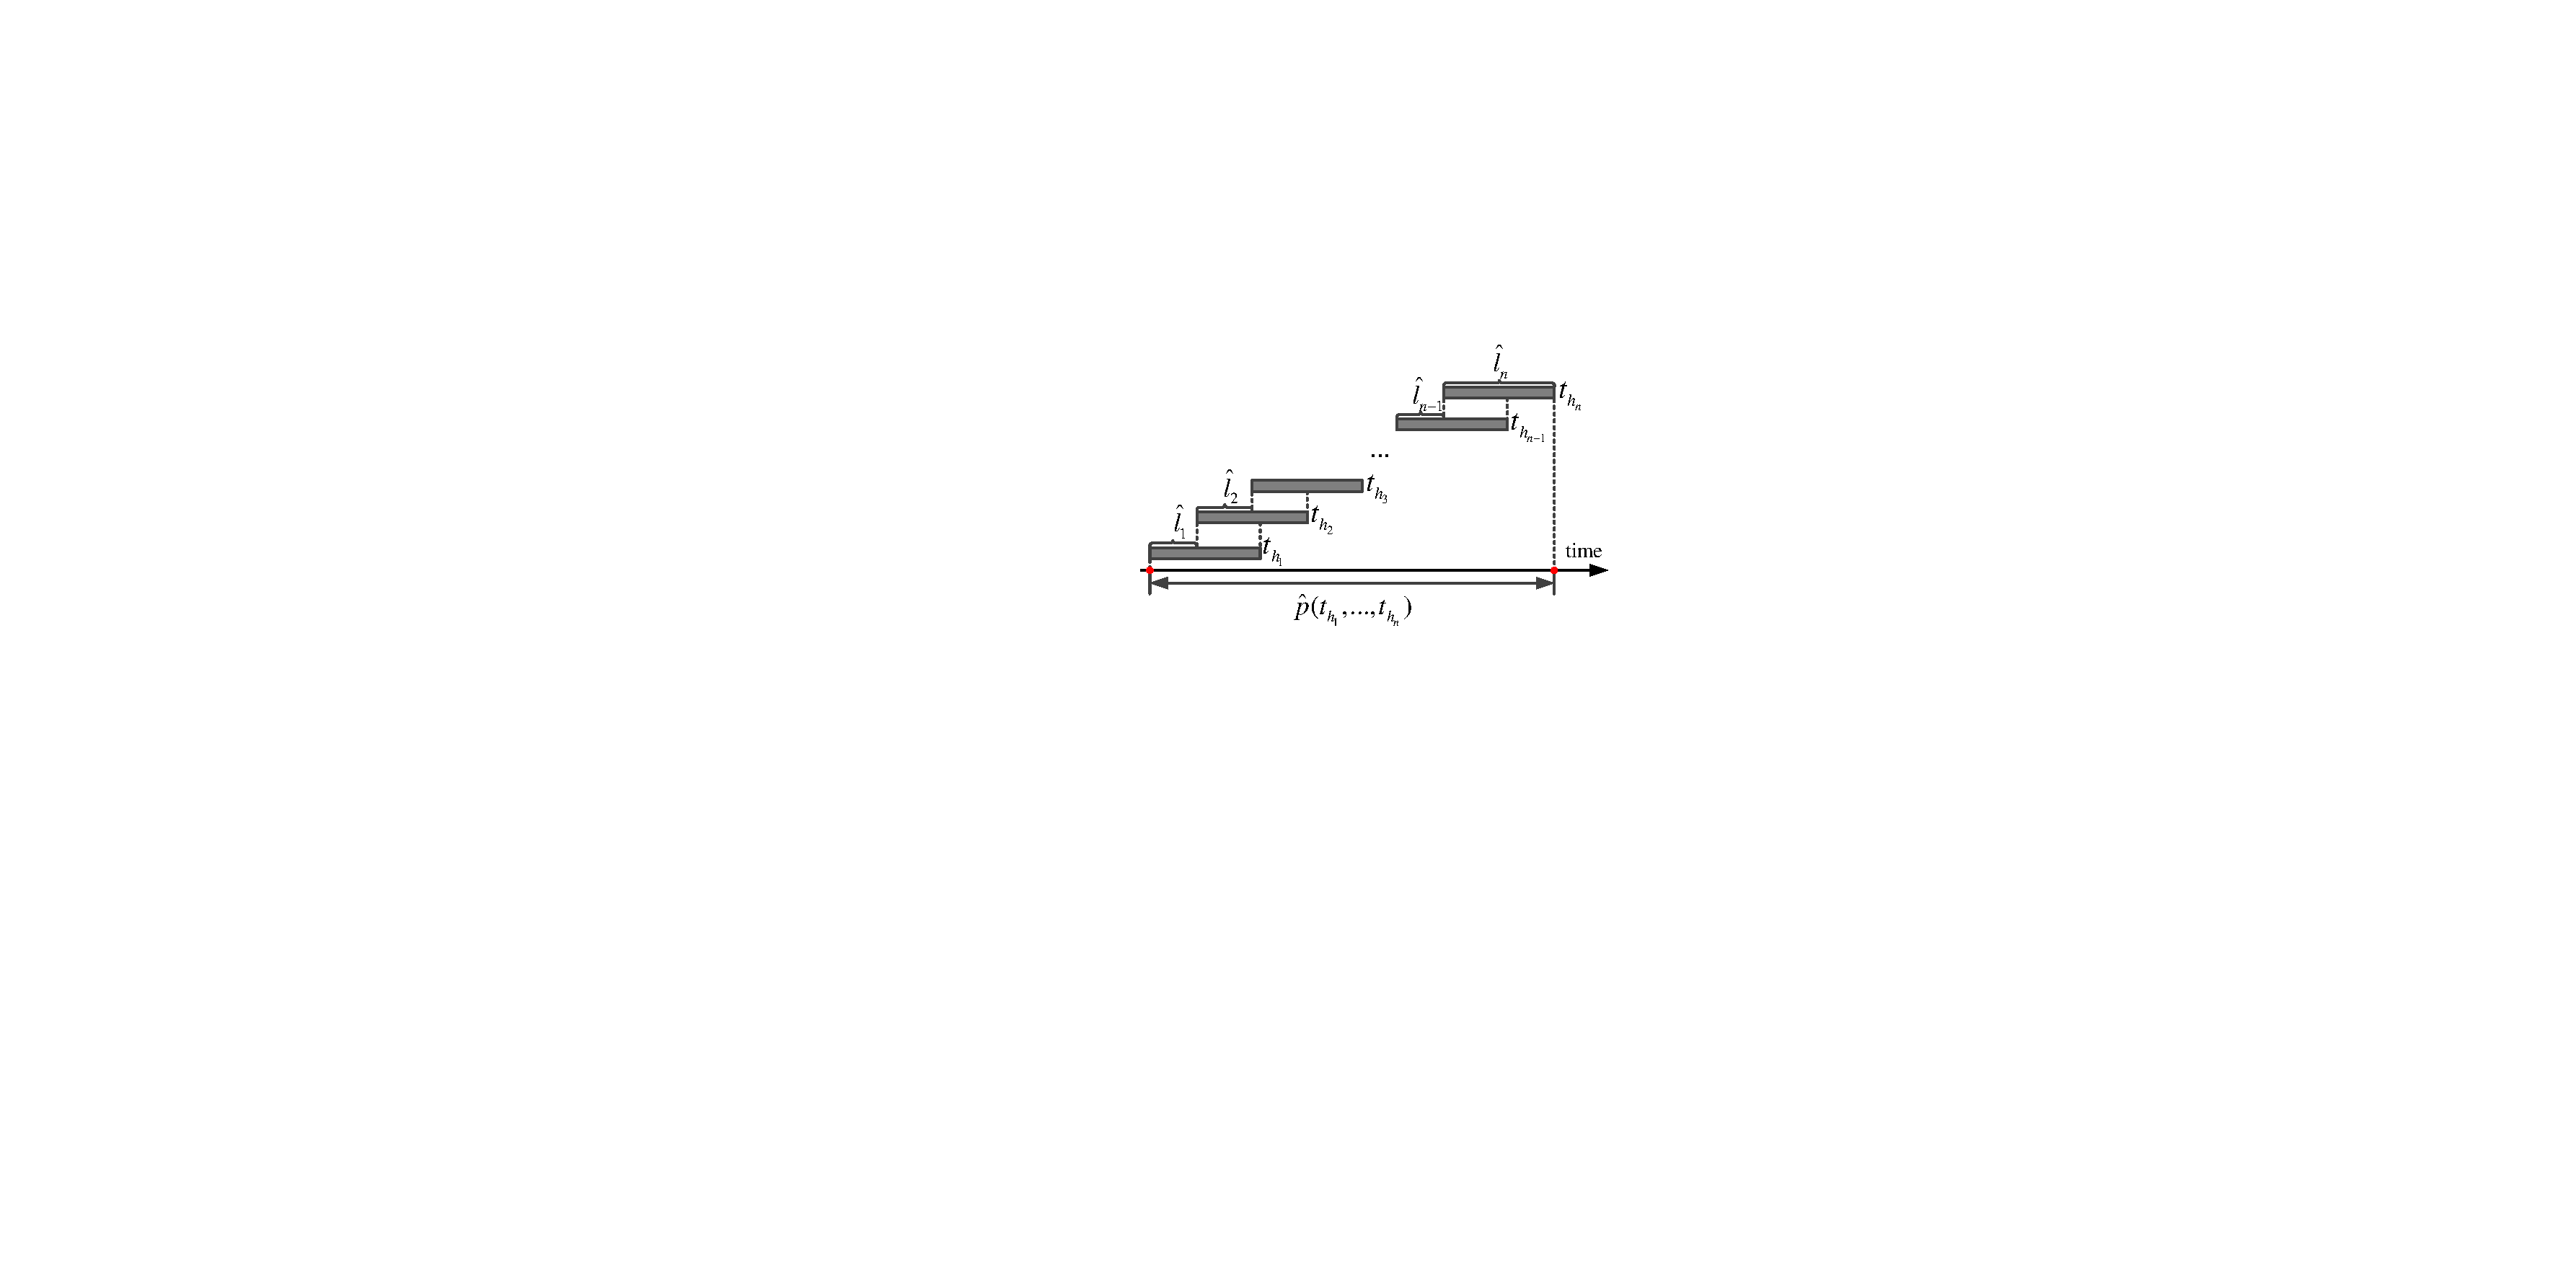
\includegraphics[width=0.43\columnwidth]{Figures/figure_proof_scheduling_2}\label{figure_proof_scheduling_2}}
\caption{MAX-DHP can be reduced to the optimization problem of  task scheduling.}
\label{figure_proof_scheduling}
\end{figure}




\begin{lemma}
\label{lemma_scheduling}
The optimization problem of task scheduling, MIN-SA, is NP complete.
\end{lemma}

\begin{proof}
Assume there is a sampling interval set $\Phi$ satisfying the requirements of tasks in $T$. Intervals in $\Phi$ are sorted in the ascending order of the begin time and $i\mathrm{=}1,2,...,|\Phi|$.

First, if $\Phi$ is the optimization solution, intervals in $\Phi$ must not be overlapping. Then, we check each interval whether it can be removed and   $\Phi$ still satisfies the left tasks. If any interval in $\Phi$ can not be removed, the solution $\Phi$ can be proved to be optimal. The process of verifying can be completed in polynomial time. Hence the  computation of the volume of sampled data is an NP problem.

Second, we construct a directional Hamilton graph which is used to reduce the Maximum Directed Hamiltonian Path (MAX-DHP) problem to the optimization problem of task scheduling. The construction procedure contains two steps:

\begin{itemize}
\item{\textbf{Step $1$: }}For any pair of tasks $t_1\mathrm{=<}b_1,e_1,l_1\mathrm{>}$ and $t_2\mathrm{=<}b_2,e_2,l_2\mathrm{>}$, if they are overlapping and $b_1\mathrm{<}b_2$, then a directed edge, pointing to $t_2$, is constructed. The weight of the edge equals the value of overlap, i.e., $d(t_1, t_2)$. If they are not overlapping, then the weight of edge is $0$. It is obvious that the interval length $l_i$ for $t_i$ can be described as $l_i \mathrm{=} d(t_i,\cdot)\mathrm{+}\widehat{l_i}$, where $d(t_i,\cdot)$ stands for the overlap between $t_i$ and other tasks. As illustrated in Fig. \ref{figure_proof_scheduling_1}, iteratively repeat the step until the directional graph $G$ is constructed.

\item{\textbf{Step $2$: }}Given any Hamilton path $t_{h_1}$, $t_{h_2}$, ..., $t_{h_n}$ in the graph $G$, the maximal length of a directed Hamilton path $p(t_{h_1}, ..., t_{h_n})$ in Fig. \ref{figure_proof_scheduling_1} is calculated as follows:

    \begin{equation}
    \begin{array}{ll}
    p(t_{h_1}, ..., t_{h_n}) \\
    = \sum^{n-1}_{i=1} {d(t_{h_i},t_{h_{i+1}})}\\
    = p(t_{h_1}, ..., t_{h_{n-1}})+(l_{t_{h_n}}-\widehat{l}_{t_{h_n}})\\
    = \cdot\cdot\cdot  \\ =\sum^{n}_{i=1}l_{t_{h_i}}-\sum^{n}_{i=1}\widehat{l}_{t_{h_i}}\\
    =\sum^{n}_{i=1}l_{t_{h_i}}-\widehat{p}(t_{h_1}, ..., t_{h_n}).
    \end{array}
    \end{equation}
    As illustrated in Fig. \ref{figure_proof_scheduling_2}, $\widehat{p}(t_{h_1},..., t_{h_n})$ is the total length of intervals for the task set. Hence the MAX-DHP problem can be reduced to the optimization problem of task scheduling, MIN-SA.
\end{itemize}
As the entire process is completed in polynomial time, Lemma \ref{lemma_scheduling} is proved.
\end{proof}


\begin{theorem}
\label{theorem_problem_allocation}
When $0 \mathrm{<} r \mathrm{<}k$, the optimization problem of task allocation, MIN-SSA,  is NP hard.
\end{theorem}

\begin{proof}
In a $k$-coverage and $r$-redundant sensor network, $r$ out of $k$ candidate nodes are used to execute a sampling task. Consider a special case, i.e., $r\mathrm{=}1$, and $k\mathrm{=}2$. In this situation, the optimization problem of task scheduling, MIN-SA, can be reduced to the optimization problem of task allocation, MIN-SSA.

Given a task set $T$ with $T \mathrm{\neq} \emptyset$, if there is an optimal solution to compute amount of the sampled data and returns an interval set $\Phi$, it is easy to divide $\Phi$ into two subsets $\Phi_1$, and $\Phi_2$ such that each of which satisfies a task subset $T_1$ and $T_2$ $(T\mathrm{=}T_1\cup T_2)$, respectively. The procedure of partition can be finished in polynomial time. However, the computation of the minimal amount of sampled data, as proved in Lemma \ref{lemma_scheduling}, is NP complete. The special case of allocation problem is NP hard. In general, the allocation problem is at least difficult as the special case. When $0 \mathrm{<} r \mathrm{<}k$, the allocation problem is thus NP hard.
\end{proof}

\subsection{Measurement of data sharing amongst tasks}
Data sharing amongst tasks is the foundation of our scheduling method. We aim at minimizing the total length of sampling intervals via the data sharing amongst overlapping tasks. Before presenting our methods, we give out some definitions.

\begin{definition}[Satisfy]
Consider two overlapping tasks $t_i\mathrm{=<}b_i,e_i,l_i\mathrm{>}$ and $t_j\mathrm{=<}b_j,e_j,l_j\mathrm{>}$. We define two variables $b$ and $e$ such that $b\mathrm{=}\max\{b_i,b_j\}$ and $e\mathrm{=}\min\{e_i,e_j\}$. Given $l_i^\ast\mathrm{=}\min\{l_i,e\mathrm{-}b\}$ and $l_j^\ast\mathrm{=}\min\{l_j,e\mathrm{-}b\}$, $t_i$ satisfies $t_j$ if and only if $l_i^\ast\mathrm{\ge} l_j$, and $t_j$ satisfies $t_i$ if and only if $l_j^\ast\mathrm{\ge} l_i$.
\label{definition_satisfy}
\end{definition}

\begin{definition}[Overlap]
Let $d(t_i,t_j)$ denote the maximal overlap value of two tasks $t_i$ and $t_j$. Without loss of generality, assume $e_i\mathrm{\le} e_j$, then:
\begin{equation}
d(t_i,t_j) \mathrm{=} \left \{ \begin{array}
{c@{\quad:\quad}l}
e_i-b_j & t_i\mathrm{,}\; t_j \; \mathrm{can}\; \mathrm{not}\; \mathrm{satisfy}\; \mathrm{each}\; \mathrm{other}.\\
l_j & t_i\; \mathrm{satisfies}\; t_j.\\
l_i & t_j\; \mathrm{satisfies}\; t_i.
\end{array} \right.
\end{equation}
\label{definition_maximal_overlap}
\end{definition}


\begin{definition}
Consider overlapping tasks $t_i\mathrm{=<}b_i,e_i,l_i\mathrm{>}$ and $t_j\mathrm{=<}b_j,e_j,l_j\mathrm{>}$. Sort those tasks in the descending order of end time. Without loss of generality, assume $e_i\mathrm{\le}e_j$. Then a time window $[b^\ast,\; e^\ast]$ can be constructed as follows:
\begin{itemize}
\item If $t_i$ and $t_j$ cannot satisfy each other, then:
\begin{equation}
\left\{ \begin{array}{ll}
b^\ast \mathrm{=} e_i\mathrm{-}l_i\\
e^\ast \mathrm{=} b_j\mathrm{+}l_j\\
\end{array} \right.
\end{equation}
\item If $t_i$ satisfies $t_j$, then:
\begin{equation}
\left\{ \begin{array}{ll}
b^\ast \mathrm{=} \max\{b_i, b\mathrm{-}(l_i\mathrm{-}l_j)\} &   b\mathrm{=}\max\{b_i,b_j\}\\
e^\ast \mathrm{=} \min\{e_i, e\mathrm{+}(l_i\mathrm{-}l_j)\}    &   e\mathrm{=}\min\{e_i,e_j\}\\
\end{array} \right.
\end{equation}
\item If $t_j$ satisfies $t_i$, then:
\begin{equation}
\left\{ \begin{array}{ll}
b^\ast \mathrm{=} \max\{b_j,b\mathrm{-}(l_j\mathrm{-}l_i)\} &   b\mathrm{=}\max\{b_i,b_j\}\\
e^\ast \mathrm{=} \min\{e_j,e\mathrm{+}(l_j\mathrm{-}l_i)\} &   e\mathrm{=}\min\{e_i,e_j\}\\
\end{array} \right.
\end{equation}
\end{itemize}
\label{definition_dominated_window}
\end{definition}


\begin{definition}[Combination]
Let $t_{ij}$ denote the combination of two overlapping tasks $t_i$ and $t_j$. The resultant task is denoted as $t^\ast$ which is called the child task, while $t_i$ and $t_j$ are called father tasks. It is clear that if $t^\ast\mathrm{=<}b^\ast,e^\ast,l^\ast\mathrm{>}$, then $l^\ast\mathrm{=}l_i\mathrm{+}l_j\mathrm{-}d(t_i,t_j)$, where both $b$ and $e$ are computed according to Definition  \ref{definition_satisfy}.
\end{definition}

%As illustrated in Fig. \ref{figure2_a}, two tasks $t_i\mathrm{=<}1,8,4\mathrm{>}$ and $t_j\mathrm{=<}5,11,5\mathrm{>}$ do not satisfy with each other. $d(t_i,t_j)\mathrm{=}3$. $b^\ast\mathrm{=}4$, $e^\ast\mathrm{=}10$. After combination of them, the resultant task is denoted as $t$ and $t\mathrm{=<}4,10,6\mathrm{>}$. In Fig. \ref{figure2_b}, two tasks $t_i\mathrm{=<}2,9,4\mathrm{>}$ and $t_j\mathrm{=<}3,11,3\mathrm{>}$ are overlapping and $t_i$ satisfies $t_j$. After combination of them, we get a new task $t\mathrm{=<}2,9,4\mathrm{>}$ where $d(t_i,t_j)\mathrm{=}3$ and $l^\ast=4$. Fig. \ref{figure2_c} shows two overlapping tasks $t_i\mathrm{=<}2,9,3\mathrm{>}$ and $t_j\mathrm{=<}3,12,5\mathrm{>}$. $t_j$ satisfies $t_i$. After combination of them, we get the resultant task $t\mathrm{=<}3,11,5\mathrm{>}$ where $d(t_i,t_j)\mathrm{=}3$ and  $l^\ast\mathrm{=}5$.
As illustrated in Fig. \ref{figure2_a}, two tasks $t_i\mathrm{=<}1,8,4\mathrm{>}$ and $t_j\mathrm{=<}5,11,5\mathrm{>}$ do not satisfy with each other. Hence, it holds that $d(t_i,t_j)\mathrm{=}3$, $b^\ast\mathrm{=}4$ and $e^\ast\mathrm{=}10$. After combination of them, a new task $t_{ij}$ is generated and $t\mathrm{=<}4,10,6\mathrm{>}$. In Fig. \ref{figure2_b}, two tasks $t_i\mathrm{=<}2,9,4\mathrm{>}$ and $t_j\mathrm{=<}3,11,3\mathrm{>}$ are overlapping and $t_i$ satisfies $t_j$. After combination of them, we get a new task $t\mathrm{=<}2,9,4\mathrm{>}$ where $d(t_i,t_j)\mathrm{=}3$ and $l^\ast=4$. Fig. \ref{figure2_c} shows two overlapping tasks $t_i\mathrm{=<}2,9,3\mathrm{>}$ and $t_j\mathrm{=<}3,12,5\mathrm{>}$, and $t_j$ satisfies $t_i$. After combination of them, we get a new task $t_{ij}$ and  $t\mathrm{=<}3,11,5\mathrm{>}$ where $d(t_i,t_j)\mathrm{=}3$ and  $l^\ast\mathrm{=}5$. In the paper, we regard the value of data sharing of sampling tasks as a metric to measure data sharing.

\begin{figure}
\centering
\subfigure[$t_i$ and $t_j$ do not satisfy with each other.]{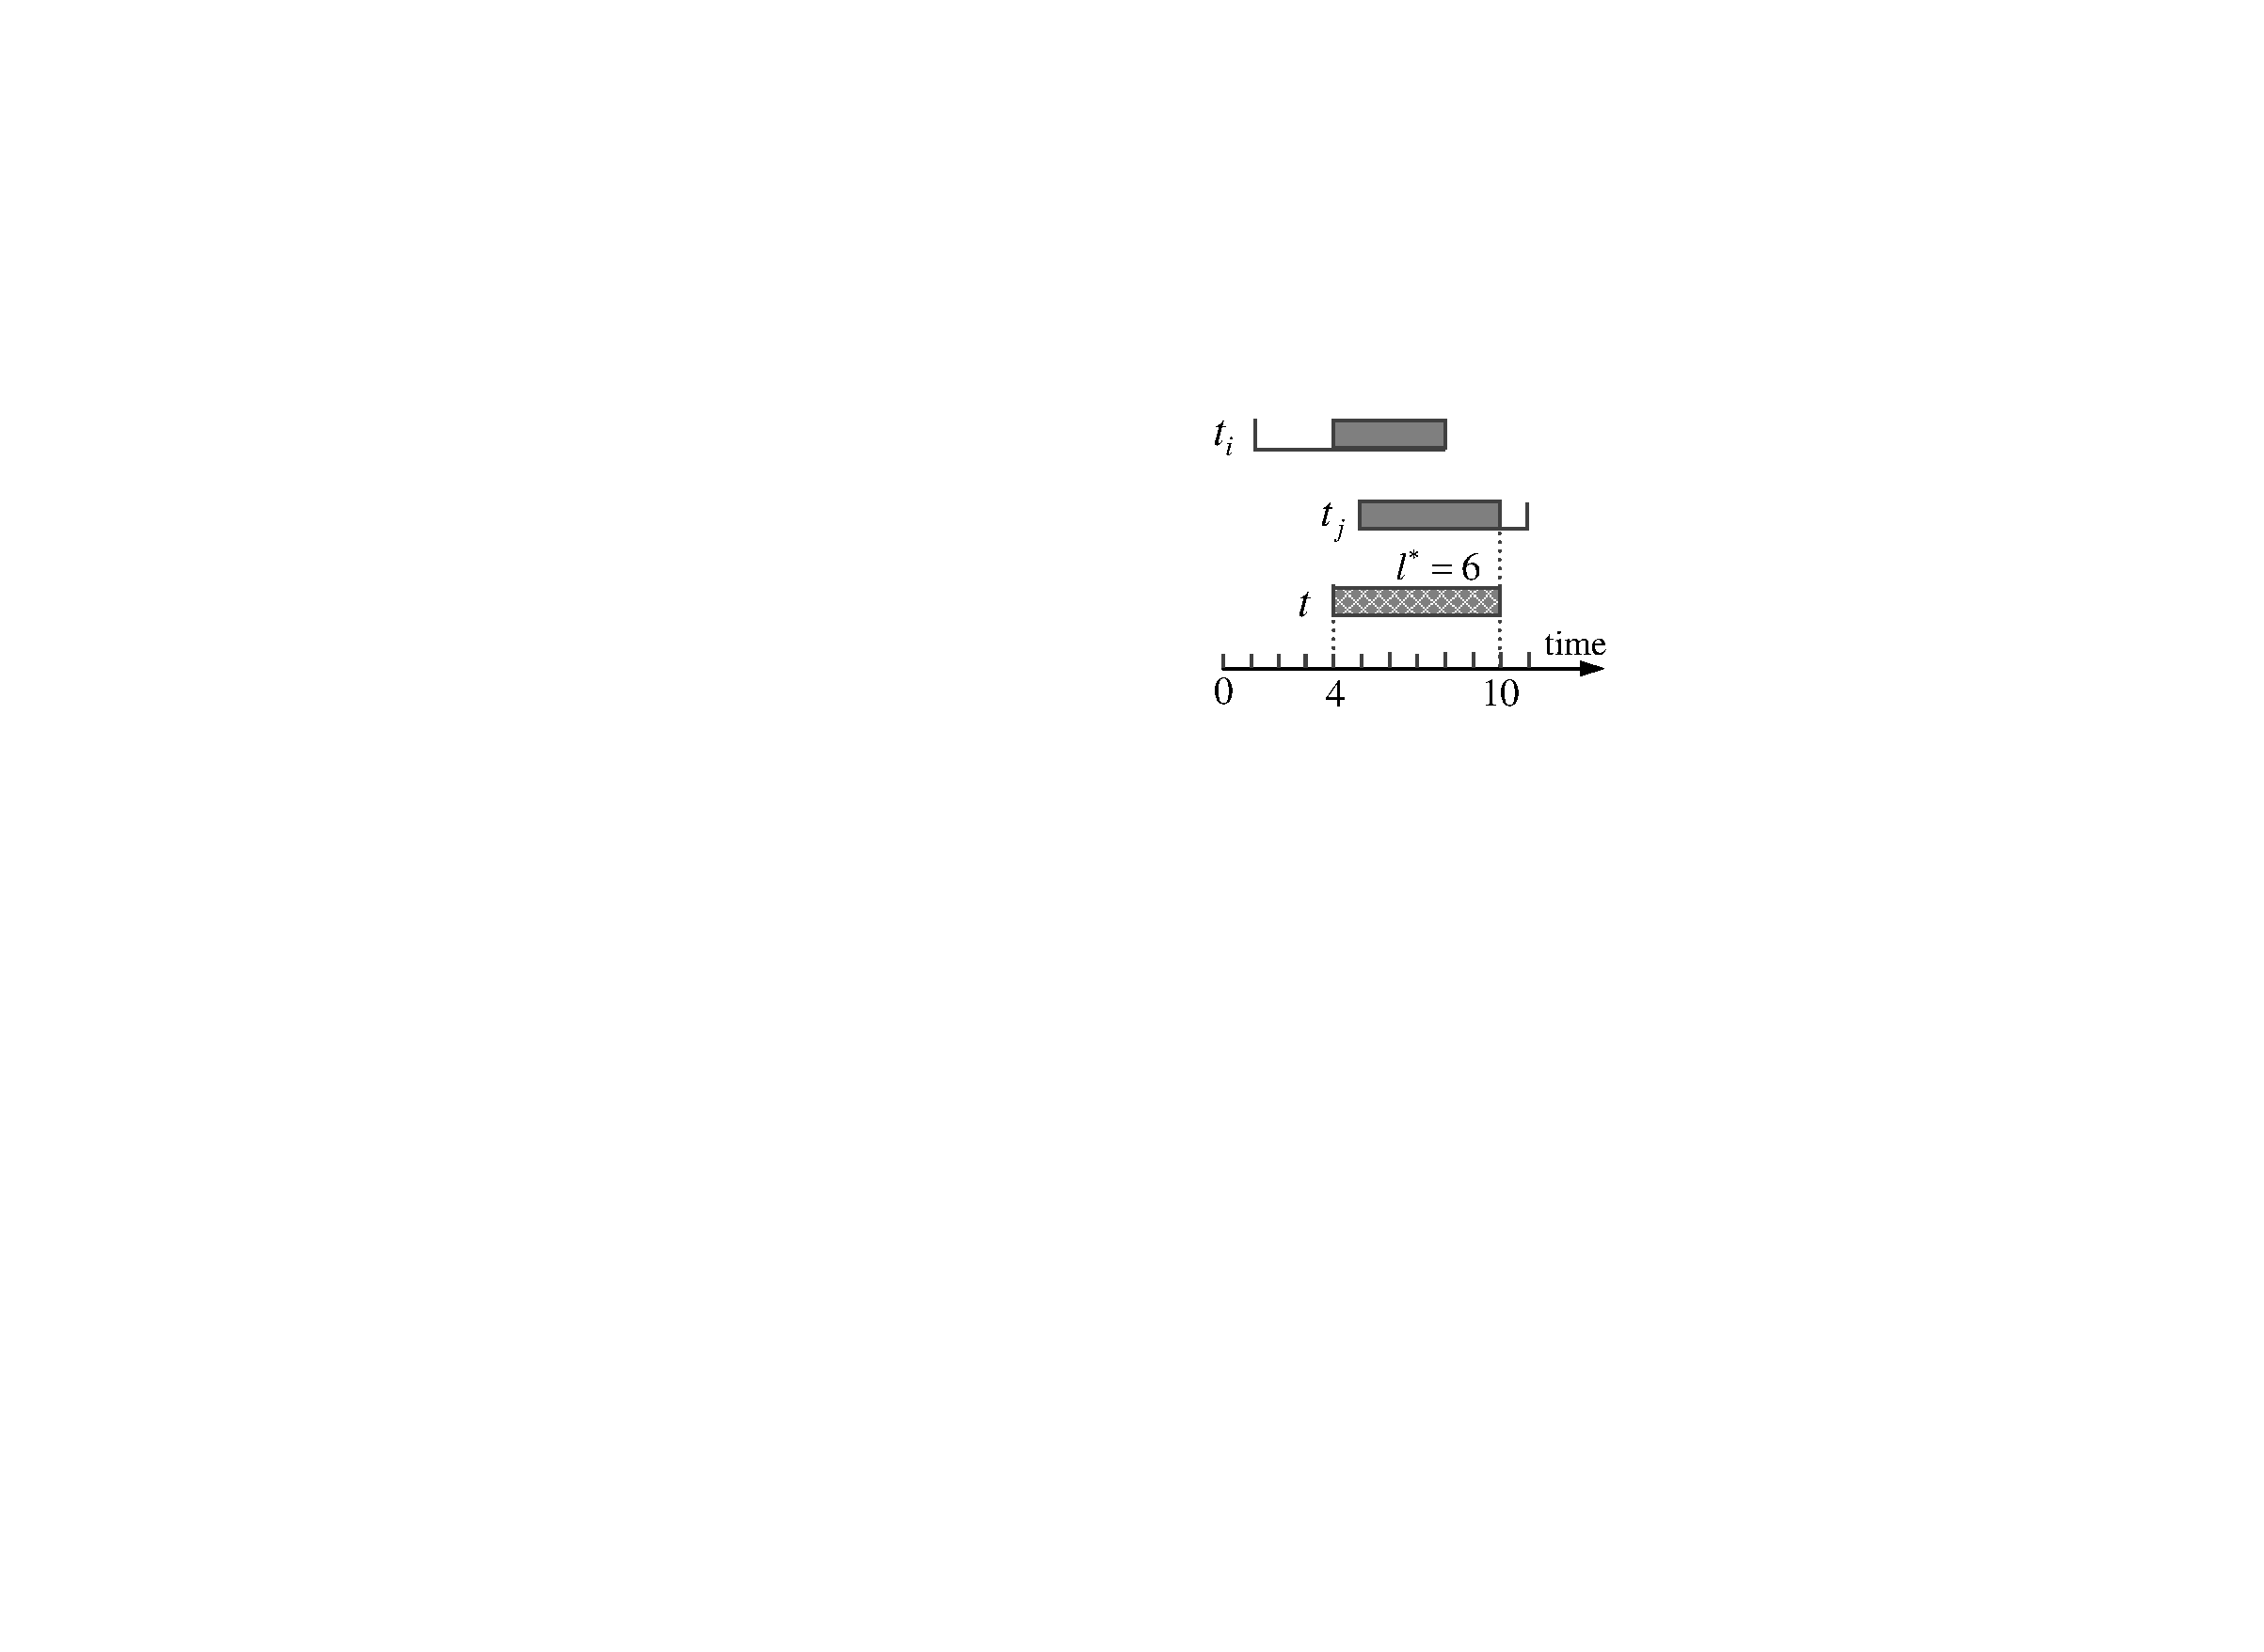
\includegraphics[width=0.23\columnwidth]{Figures/figure2_a}\label{figure2_a}}
\hspace{2pt}
\subfigure[$t_i$ satisfies $t_j$.]{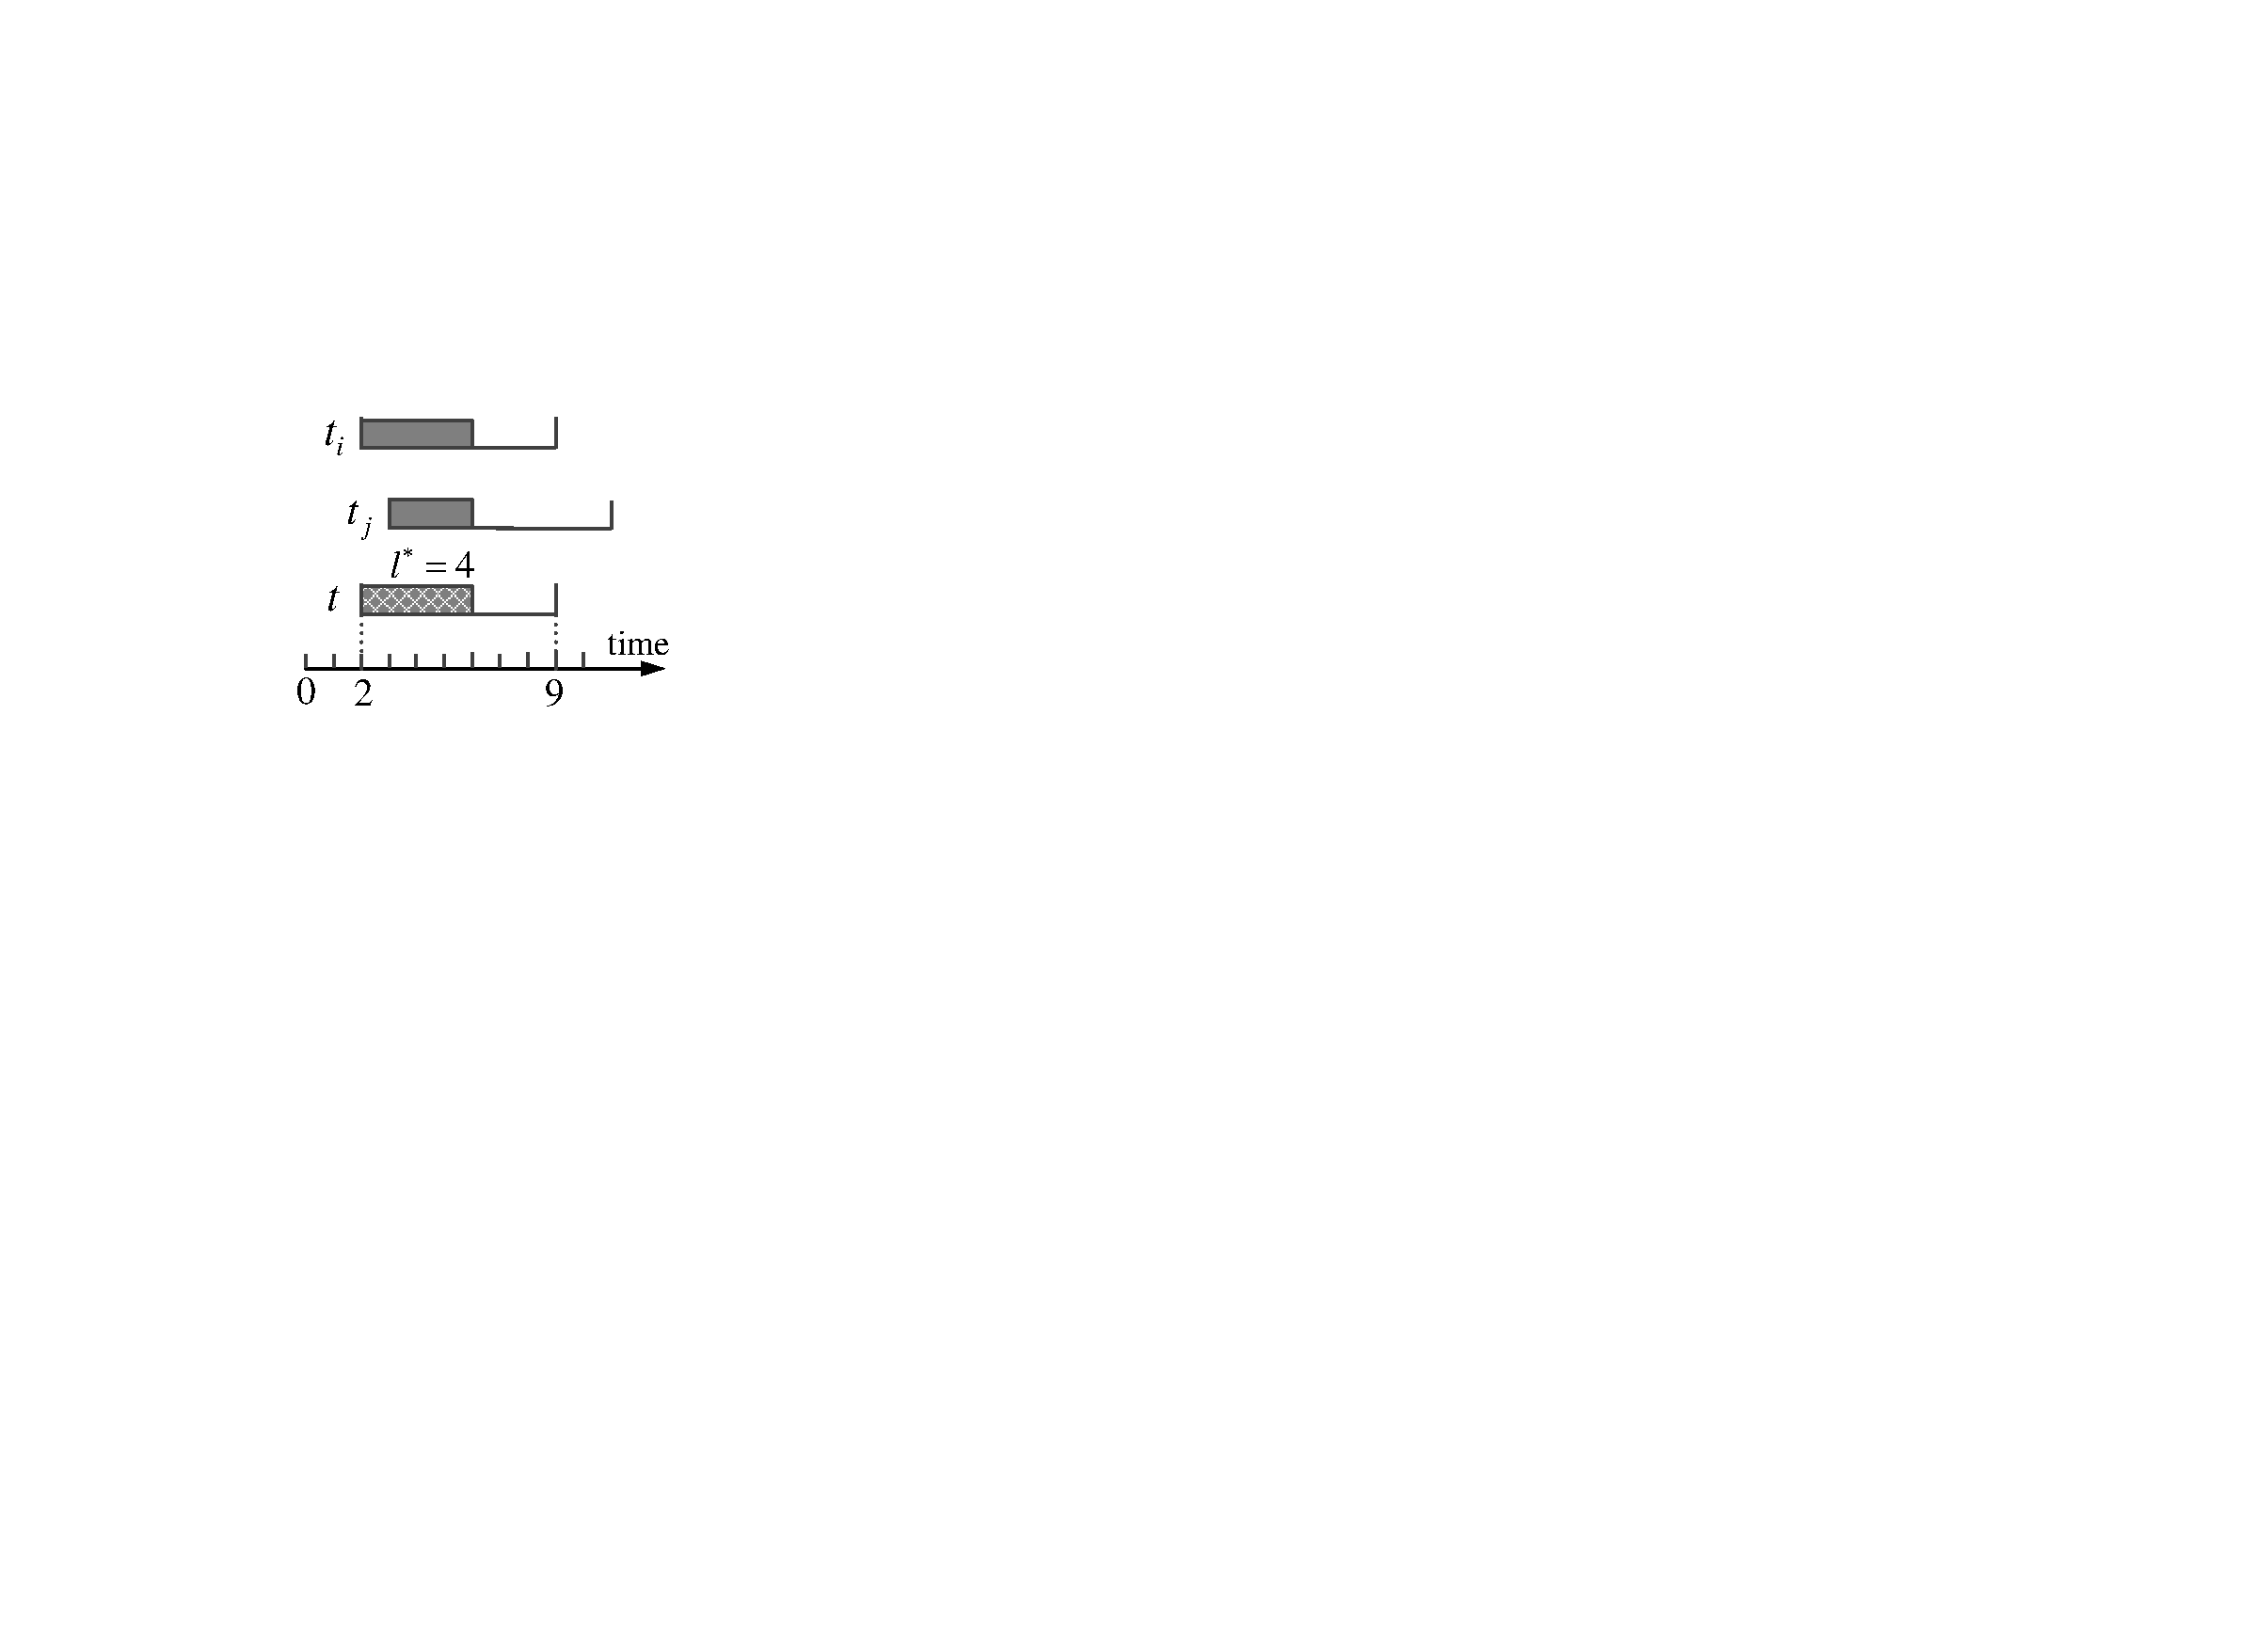
\includegraphics[width=0.23\columnwidth]{Figures/figure2_b}\label{figure2_b}}
\hspace{2pt}
\subfigure[$t_j$ satisfies $t_i$. ]{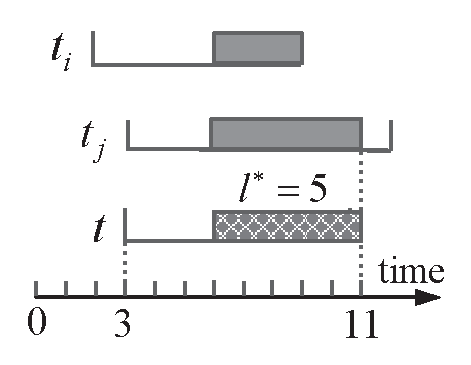
\includegraphics[width=0.23\columnwidth]{Figures/figure2_c}\label{figure2_c}}
\caption{Three cases: the combination of overlapping tasks.}
\label{figure_combination}
\end{figure}


\section{A 2-factor approximation scheduling algorithm designing for a sampling task set}
\label{section_schedule}
In this section, we first propose a task scheduling algorithm for a task set via the data sharing amongst the overlapping tasks, and then prove it 2-factor approximation by the theoretical analysis.

Let $T$ denote a non-empty task set at a sensor node. If $|T|\mathrm{=}1$, the amount of sampled data is determined solely. If $|T|\mathrm{>}1$, a quad $q\mathrm{=<}t_i,t_j,t,d(t_i,t_j)\mathrm{>}$ is maintained for the combination of the overlapping tasks, i.e., $t_i$ and $t_j$. Here,  $t_i$ and $t_j$ are father tasks,  $t$ is the combination result of $t_i$ and $t_j$, and $d(t_i,t_j)$ is the maximal overlap value.

Our basic idea is to schedule all tasks in $T$ by iteratively combining the task pair which has the maximal overlap value until there are no overlapping tasks in $T$. The whole scheduling procedure includes three major steps. First, it computes the combination of all overlapping tasks and gets a quad list $Q$. Second, the quad $q$, $q\mathrm{\in} Q$, whose $d(t_i,t_j)$ is maximal is found. The original tasks $t_i$ and $t_j$ are replaced by the new task $t$ in the task set  $T$. Third, repeat above steps until no tasks are overlapping. Algorithm \ref{algorithm_combine} presents the details and returns a task set which has no overlapping sampling tasks.

\begin{algorithm}[t]
	\SetAlgoNoLine
	\KwIn{A task set $T$ and $T\mathrm{\neq}\emptyset$.}
	\KwOut{A task set where there are no overlapping tasks.}
    \caption{Combine}
    \label{algorithm_combine}
    %\begin{algorithmic}[1]
        sort tasks in $T$ in the descending order of end time\;
        $Q\mathrm{\leftarrow}$ Pre\_processing $(T)$\;
        sort quads in $Q$ in the descending order of value of data sharing\;
        \Repeat {$|T|\mathrm{>}1$ and $T$ contains overlapping tasks}{
            $t_i\mathrm{=}Q(0).t_i$, $t_j\mathrm{=}Q(0).t_j$, $t_{ij}\mathrm{=}Q(0).t_{ij}$\;
            insert $t_{ij}$ into $T$ in the ascending order of  end time\;
            remove $t_i$ and $t_j$ from $T$ and quads which include $t_i$ or $t_j$ from $Q$\;
        }
        \Return $T$\;

        \textbf{Function:} Pre\_processing ($T$)\\
%            \KwIn{A task set $T$ and $T\mathrm{\neq}\emptyset$.}
%	        \KwOut{A quad list where each quad consists of two overlapping tasks.}
        \Repeat {each task $t_i$ in $T$}{
            \Repeat {each task $t_j\mathrm{\in} T\mathrm{-}\{t_i\}$}{
                \If {$t_i$ is overlapping with $t_j$}
                    {a quad $q$ is generated with $q\mathrm{=}\mathrm{<}t_i,t_j,t_{ij},d(t_i,t_j)\mathrm{>}$\;
                   $Q \mathrm{\leftarrow}Q\mathrm{\bigcup}\{q\}$\;}
            }
        }
        \Return $Q$\;
%        \EndFunction
    %\end{algorithmic}
\end{algorithm}

\begin{figure}[t]
\centering
\subfigure[Value of data sharing between overlapping tasks.]{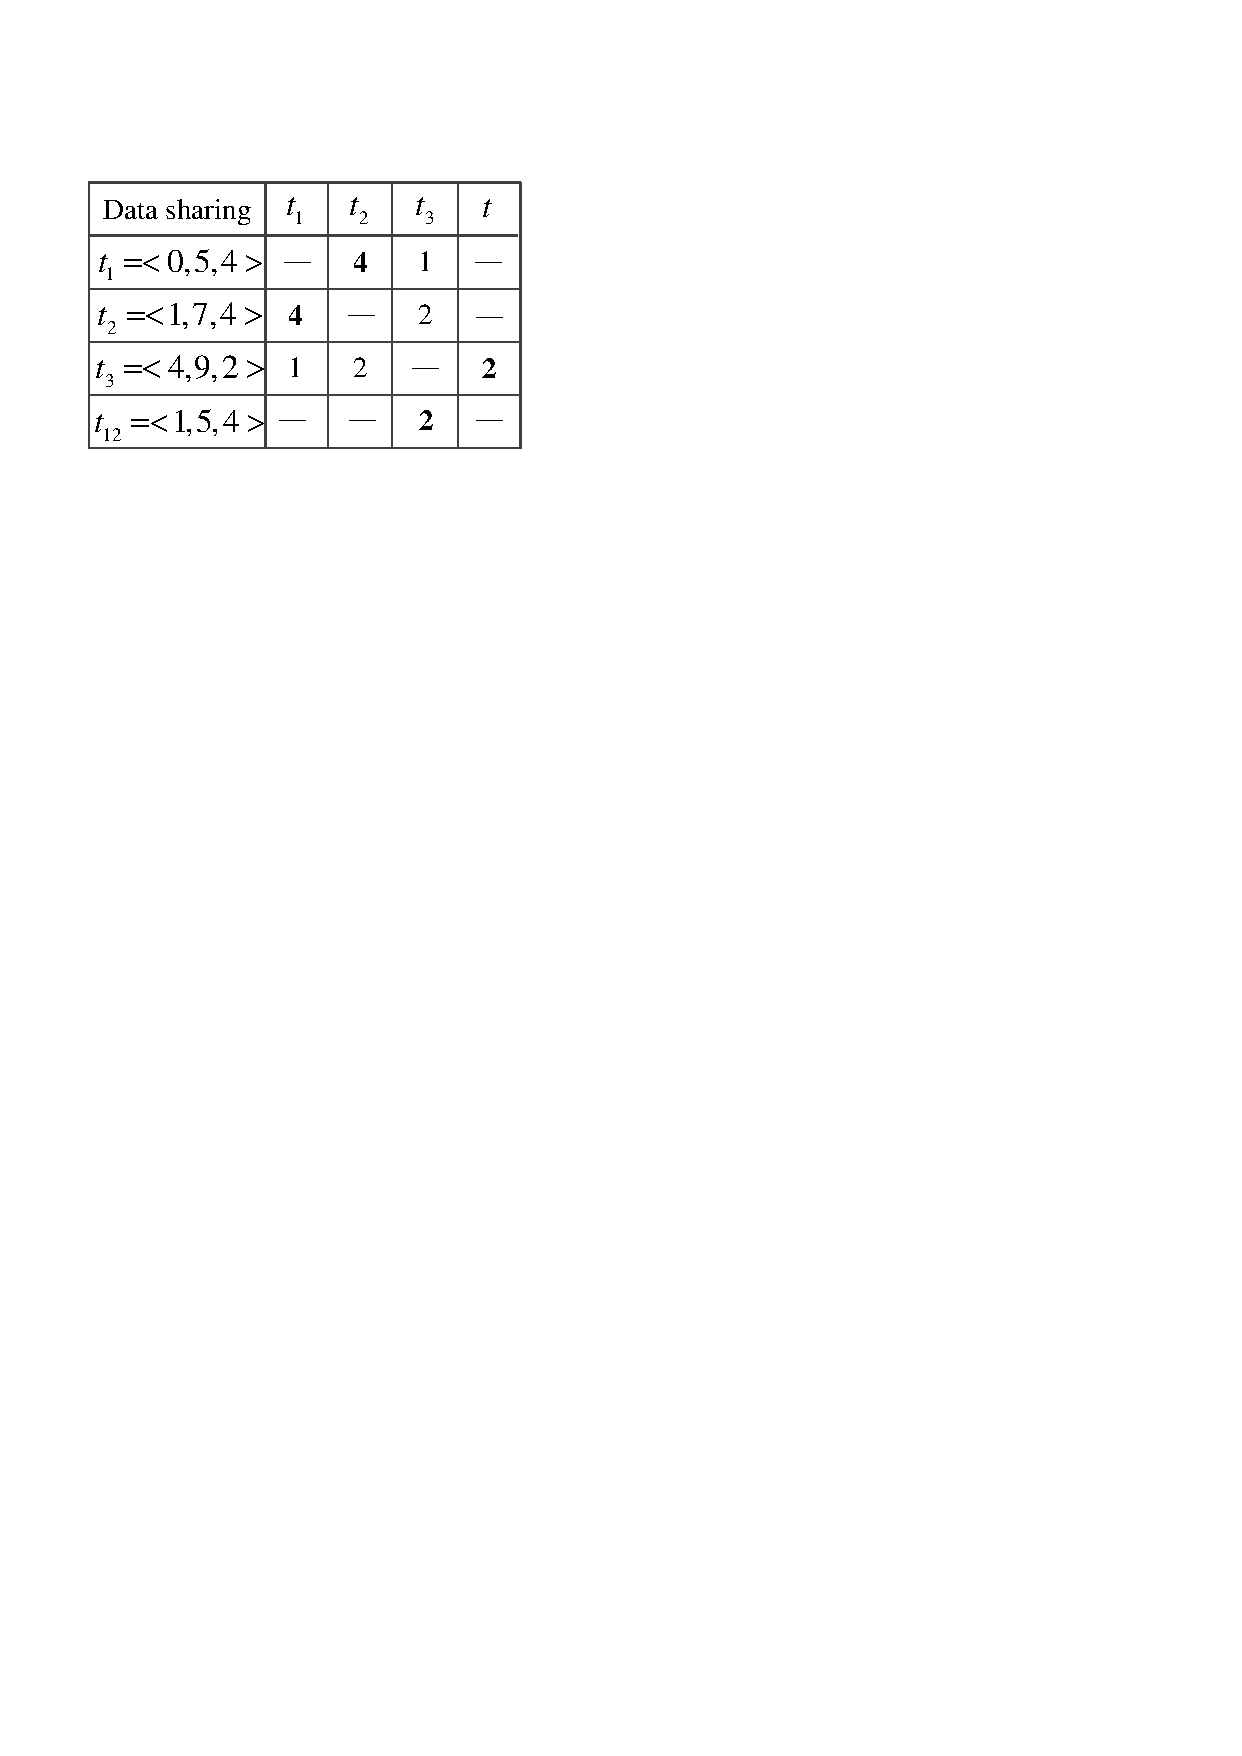
\includegraphics[width=0.28\columnwidth]{Figures/figure_combination_overlap}\label{figure_combination_overlap}}
\hspace{3pt}
\subfigure[Combination of tasks in the descending order of value of data sharing.]{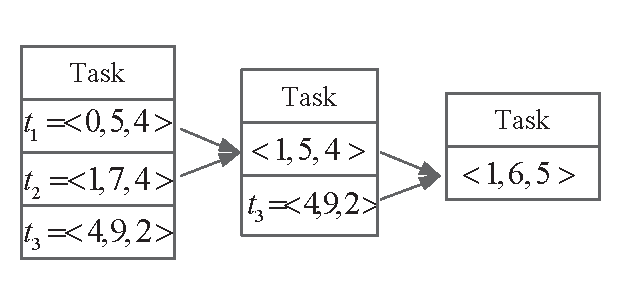
\includegraphics[width=0.35\columnwidth]{Figures/figure_combination_combine}\label{figure_combination_combine}}
\caption{The process of combination for overlapping tasks.}
\label{figure_combination}
\end{figure}
%Algorithm \ref{algorithm_combine} performs an iterative operation. Lines $1\mathrm{-}3$ initialize a quad list $Q$, and sort the quad list in the order of $d(t_i,t_j)$. It consumes $O(n^2)$ memory to maintain the quad list. The time complexity is $O(n^2)$ due to the computation of  maximal overlap value. Lines $4\mathrm{-}7$  find a task pair which have the maximal overlap value in the task set $T$, and then update $T$ and $Q$. Note that both the space complexity and time complexity of Algorithm \ref{algorithm_combine} are $O(n^2)$. As shown in Table \ref{table_combine}, three tasks are notated as $t_1\mathrm{=<}0,4,3\mathrm{>}$, $t_2\mathrm{=<}2,7,3\mathrm{>}$ and $t_3\mathrm{=<}4,9,2\mathrm{>}$. First, we compute the length of the overlapping intervals and find that $t_1$ and $t_2$ have the maximal overlap value $d(t_1,t_2)\mathrm{=}4$. Then, $t_1$ and $t_2$ are selected to construct a new task $t\mathrm{=<}1,5,4\mathrm{>}$. Second, remove $t_1$ and $t_2$ from $T$ and add $t$ into $T$. In the next round, $t$ and $t_3$ is overlapping and will be combined. We finally get the resultant task, i.e., $\mathrm{<}1,6,5\mathrm{>}$ after combining $t$ and $t_3$. So the final sampling interval is $[1,6]$, and the amount of sampled data is $5$.

Algorithm \ref{algorithm_combine} performs an iterative operation. Lines $1\mathrm{-}3$ initialize a quad list $Q$, and sort the quad list in the descending order of $d(t_i,t_j)$. It consumes $O(n^2)$ memory to maintain the quad list. The time complexity is $O(n^2)$ due to the computation of  maximal value of data sharing. Lines $4\mathrm{-}7$  find a task pair which has the maximal value of data sharing in the task set $T$, and then update $T$ and $Q$.  As shown in Fig. \ref{figure_combination}, three tasks are notated by $t_1\mathrm{=<}0,5,4\mathrm{>}$, $t_2\mathrm{=<}1,7,4\mathrm{>}$ and $t_3\mathrm{=<}4,9,2\mathrm{>}$. First, we compute the data sharing of overlapping tasks and find that $t_1$ and $t_2$ have the maximal value of data sharing $d(t_1,t_2)\mathrm{=}4$. Then, $t_1$ and $t_2$ are selected to construct a new task $t_{12}\mathrm{=<}1,5,4\mathrm{>}$. Second, remove $t_1$ and $t_2$ from $T$ and add $t_{12}$ into $T$.  We get a new task, i.e., $\mathrm{<}1,6,5\mathrm{>}$ after combining $t_{12}$ and $t_3$. Hence, the final sampling interval is $[1,6]$, and the amount of sampled data is $5$.



Note that both the space complexity and time complexity of Algorithm \ref{algorithm_combine} are $O(n^2)$. Consider that the memory resource is very rare for a wireless sensor node. Algorithm \ref{algorithm_combine} costs $O(n^2)$ space complexity because of maintaining a quad list. To address this problem, we further propose Algorithm \ref{algorithm_combine2} whose space complexity is $O(n)$ and time complexity is $O(n^2)$.  It exhibits the same performance with Algorithm \ref{algorithm_combine}, but significantly reduces the memory consumption. Algorithm \ref{algorithm_combine} is proved to be a 2-factor approximation task scheduling algorithm by Theorem \ref{theorem_schedule}. Before presenting the Theorem \ref{theorem_schedule}, we first present Lemma \ref{lemma1} and Property \ref{property1} which will be used in the proof of Theorem \ref{theorem_schedule}.

\begin{algorithm}[t]
	\SetAlgoNoLine
	\KwIn{A task set $T$ and $T\mathrm{\neq}\emptyset$.}
	\KwOut{A task set where there are no overlapping tasks.}
    \caption{Combine\_2}
    \label{algorithm_combine2}
    %\begin{algorithmic}[1]
        sort tasks in $T$ in the ascending order of end time\;
        \Repeat {$|T|\mathrm{>}1$ and $T$ contains overlapping tasks}{
            find a task pair $\mathrm{<}t_i,t_j\mathrm{>}$ with the maximal overlap\;
            insert the resultant task, i.e.,  $t=t_{ij}$ into $T$ in the ascending order of end time\;
            remove $t_i$ and $t_j$ from $T$\;
        }
        return $T$\;
    %\end{algorithmic}
\end{algorithm}

\begin{lemma}
\label{lemma1}
For a non-empty task set $T$, if the selected two tasks from the task set by Algorithm \ref{algorithm_combine} are $t_i$ and $t_j$, the combination of such two tasks generates a new task $t\mathrm{=}t_{ij}$. For any other task $t_k  \mathrm{\in} T$, we have $d(t_i,t_j) \mathrm{\geq} \mathrm{\max} \{$$d(t_i,t_k)$, $d(t_j,t_k)$$\}$ and $d(t,t_k)\mathrm{\le}\min\{d(t_i,t_k)$, $d(t_j,t_k)\}$.
\end{lemma}

\begin{proof}
Note that $t_i$ and $t_j$ are the selected candidate tasks by Algorithm \ref{algorithm_combine}. It means that for a task set $T$, the current maximal overlap value is $d(t_i,t_j)$. Without loss of generality, we assume $d(t_i,t_k)\mathrm{\ge} d(t_j,t_k)$.

First, there exists a task notated as $t_k$. $t_k \mathrm{\in} T$, $t_k \mathrm{\neq} t_i$, $t_k \mathrm{\neq} t_j$. If $d(t_i,t_j)\mathrm{<}d(t_i,t_k)$, then the value of overlap between tasks $t_i$ and $t_j$ is not the maximal. It is a contradiction because we compute the current maximal overlap value by Algorithm \ref{algorithm_combine}. Thus, we have $d(t_i,t_j)\mathrm{\geq} d(t_i,t_k)$.

Second, if a task $t$ is the resultant task by the combination of tasks $t_i$ and $t_j$, i.e., $t\mathrm{=}t_{ij}$, then $d(t,t_k)\mathrm{=}d(t_i,t_j,t_k)$. Since $d(t_i,t_j,t_k)\mathrm{\le} d(t_j,t_k)$ is always satisfied, we have $d(t,t_k)\mathrm{\le} d(t_j,t_k)$.
\end{proof}

\begin{lemma}
\label{property1}
The overlap value between two tasks, according to Algorithm \ref{algorithm_combine}, is monotone non-increasing.
\end{lemma}

\begin{proof}
Consider a non-empty task set $T$  and the overlapping tasks $t_i$ and $t_j$. For $\forall t_k \mathrm{\in} T$, $d(t_i,t_j)\mathrm{\ge}o(t_{ij},t_k)$ always establishes according to Lemma \ref{lemma1}. Then we can prove the Lemma \ref{property1} by using the method of mathematical induction. Since we identify  a task pair with the maximal overlap value from the task set $T$ in each combination step. If $t_{ij}$ is the current choice, it means other task pairs cannot provide more data sharing than $t_i$ and $t_j$ in the current step. After the combination step, if a further task pair is $t_x$ and $t_y$, we have $d(t_x,t_y)\mathrm{\le} d(t_i,t_j)$  according to Lemma \ref{lemma1}. Thus Lemma \ref{property1} is proved.
\end{proof}

\begin{definition}[Compact model of a task]
For a task $t_i\mathrm{=<}b_i,e_i,l_i\mathrm{>}$, let $\widetilde{t_i}\mathrm{=<}\widetilde{b},\widetilde{e},\widetilde{l}>$ denote its compact model such that:
\begin{equation}
\left\{ \begin{array}{ll}
\widetilde{b} = b_i\\
\widetilde{e} = e_i\\
l_i = e_i\mathrm{-}b_i
\end{array} \right.
\end{equation}
\end{definition}

\begin{definition}[Compact model of a task set]
For a task set $T\mathrm{=}\{t_1,...,t_n\}$ where $t_i\mathrm{=<}b_i,e_i,l_i\mathrm{>}$ and $1\mathrm{\le} i\mathrm{\le} n$, its compact model consists of $\varphi$ compact tasks which are not overlapping with each other. These compact tasks $\widetilde{t_1}, \widetilde{t_2}, ..., \widetilde{t_\varphi}$ have the same interval length $\delta$ such that:

\begin{equation}
\left\{ \begin{array}{ll}
\delta \le \min\{l_1,l_2,...,l_n\}, \ \delta \ is \ a \ positive \ constant.\\
\varphi=\min\{x|x\mathrm{\cdot}\delta\mathrm{\ge} \sum_{i\mathrm{=}1}^{n}l_i,\ x\ is\ a\ positive\ integer.\}
\end{array} \right.
\end{equation}
\end{definition}


%\begin{figure}
%\centering
%\subfigure[A sampling task set]{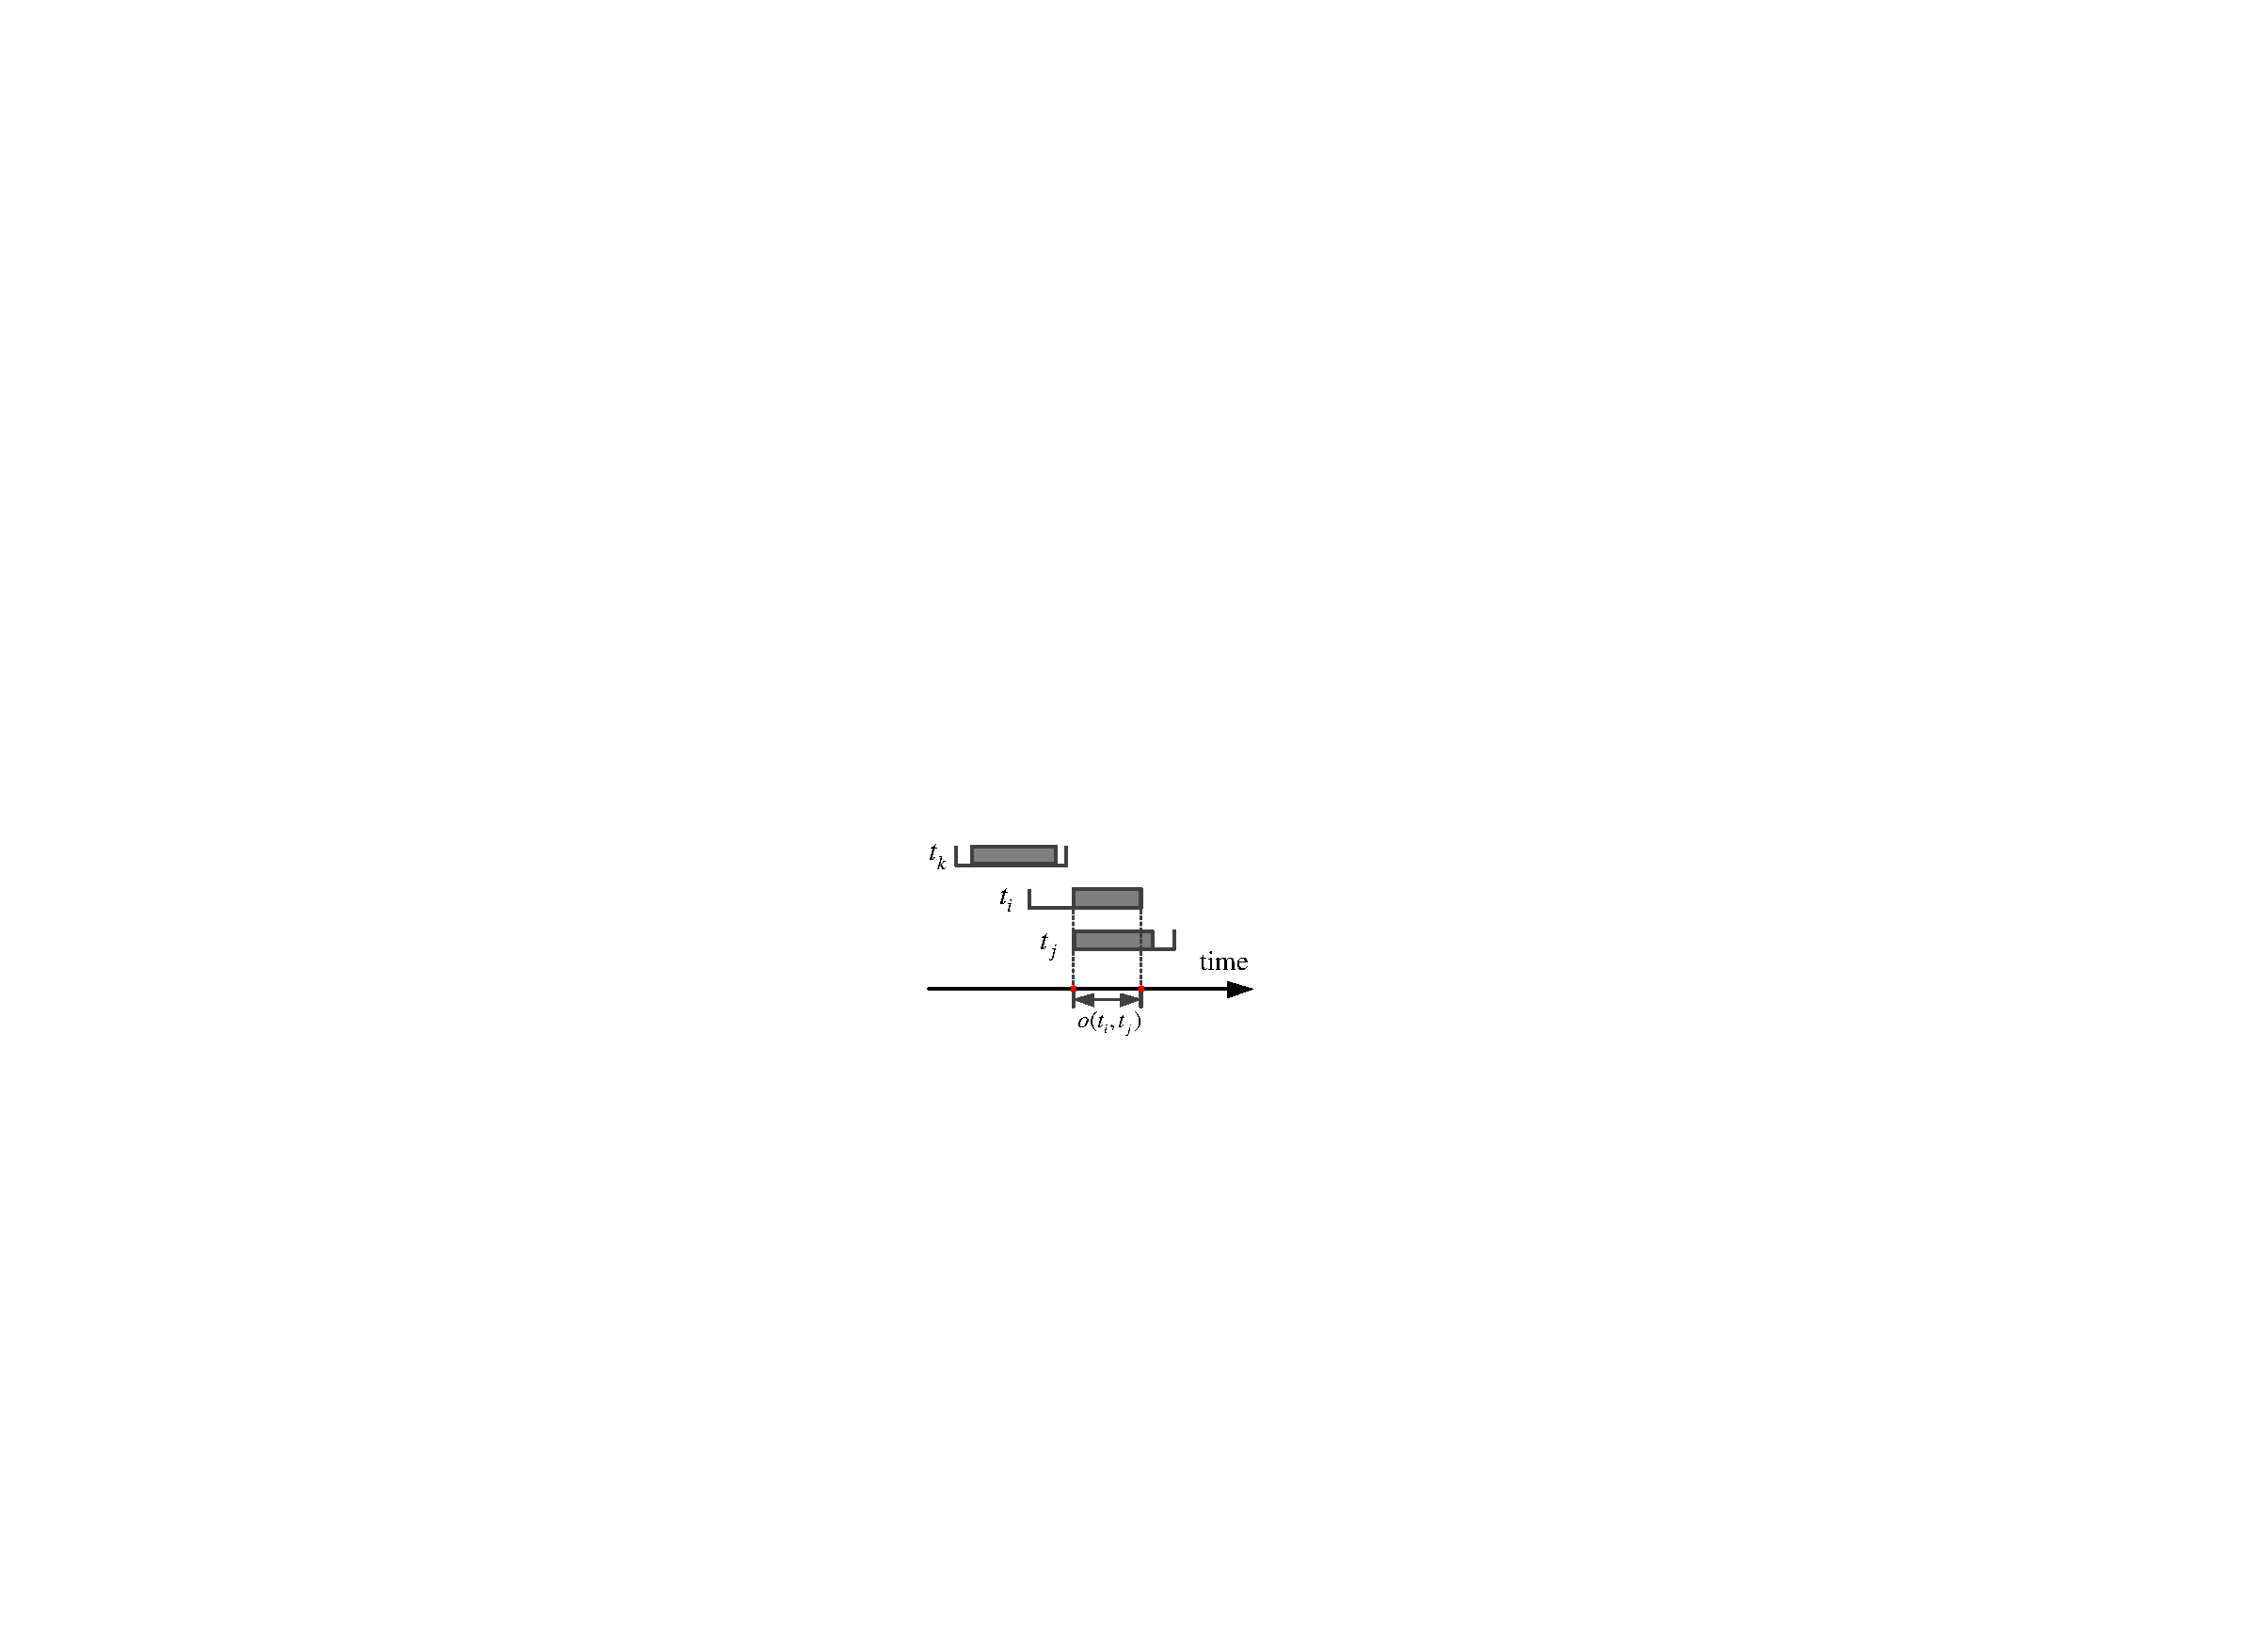
\includegraphics[width=0.45\columnwidth]{Figures/figure_proof_scheduling_origin}\label{figure_proof_scheduling_origin}}
%\subfigure[Its compact model]{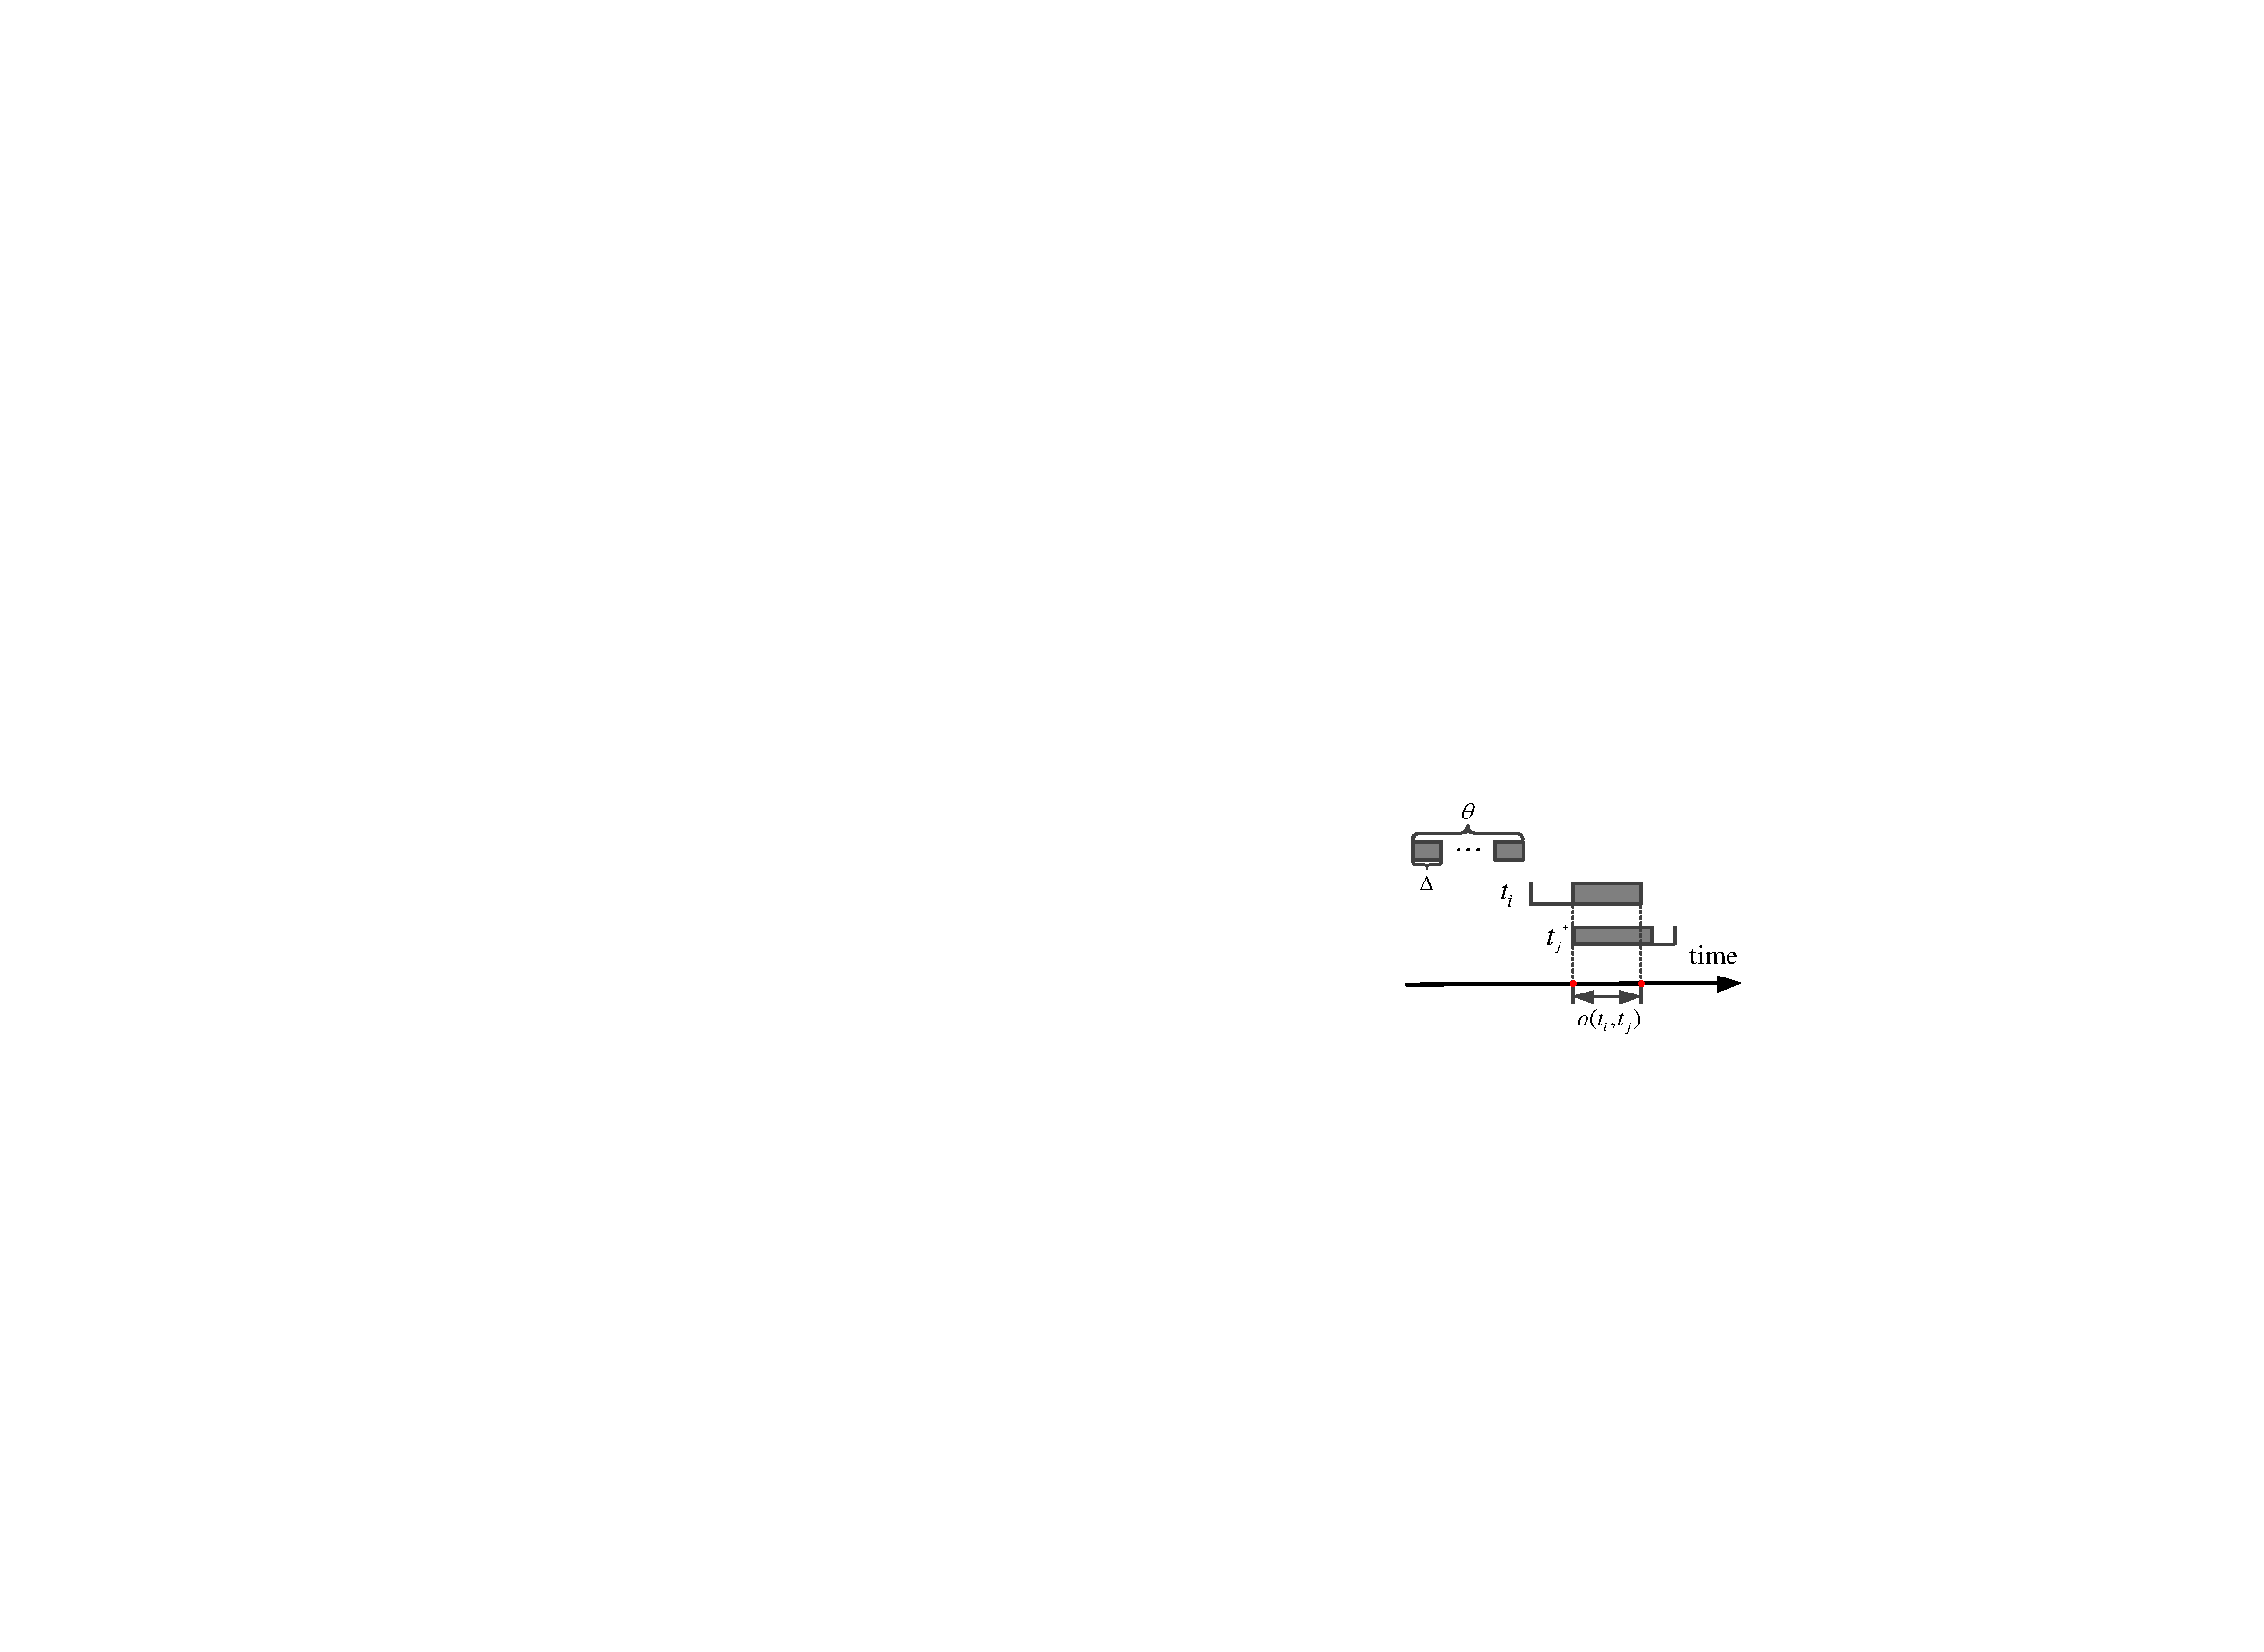
\includegraphics[width=0.46\columnwidth]{Figures/figure_proof_scheduling_model}\label{figure_proof_scheduling_model}}
%\caption{A sampling task set and its compact model.}
%\label{figure_proof_scheduling_performance}
%\end{figure}
%
%\begin{figure}
%\centering
%\subfigure[Greedy result]{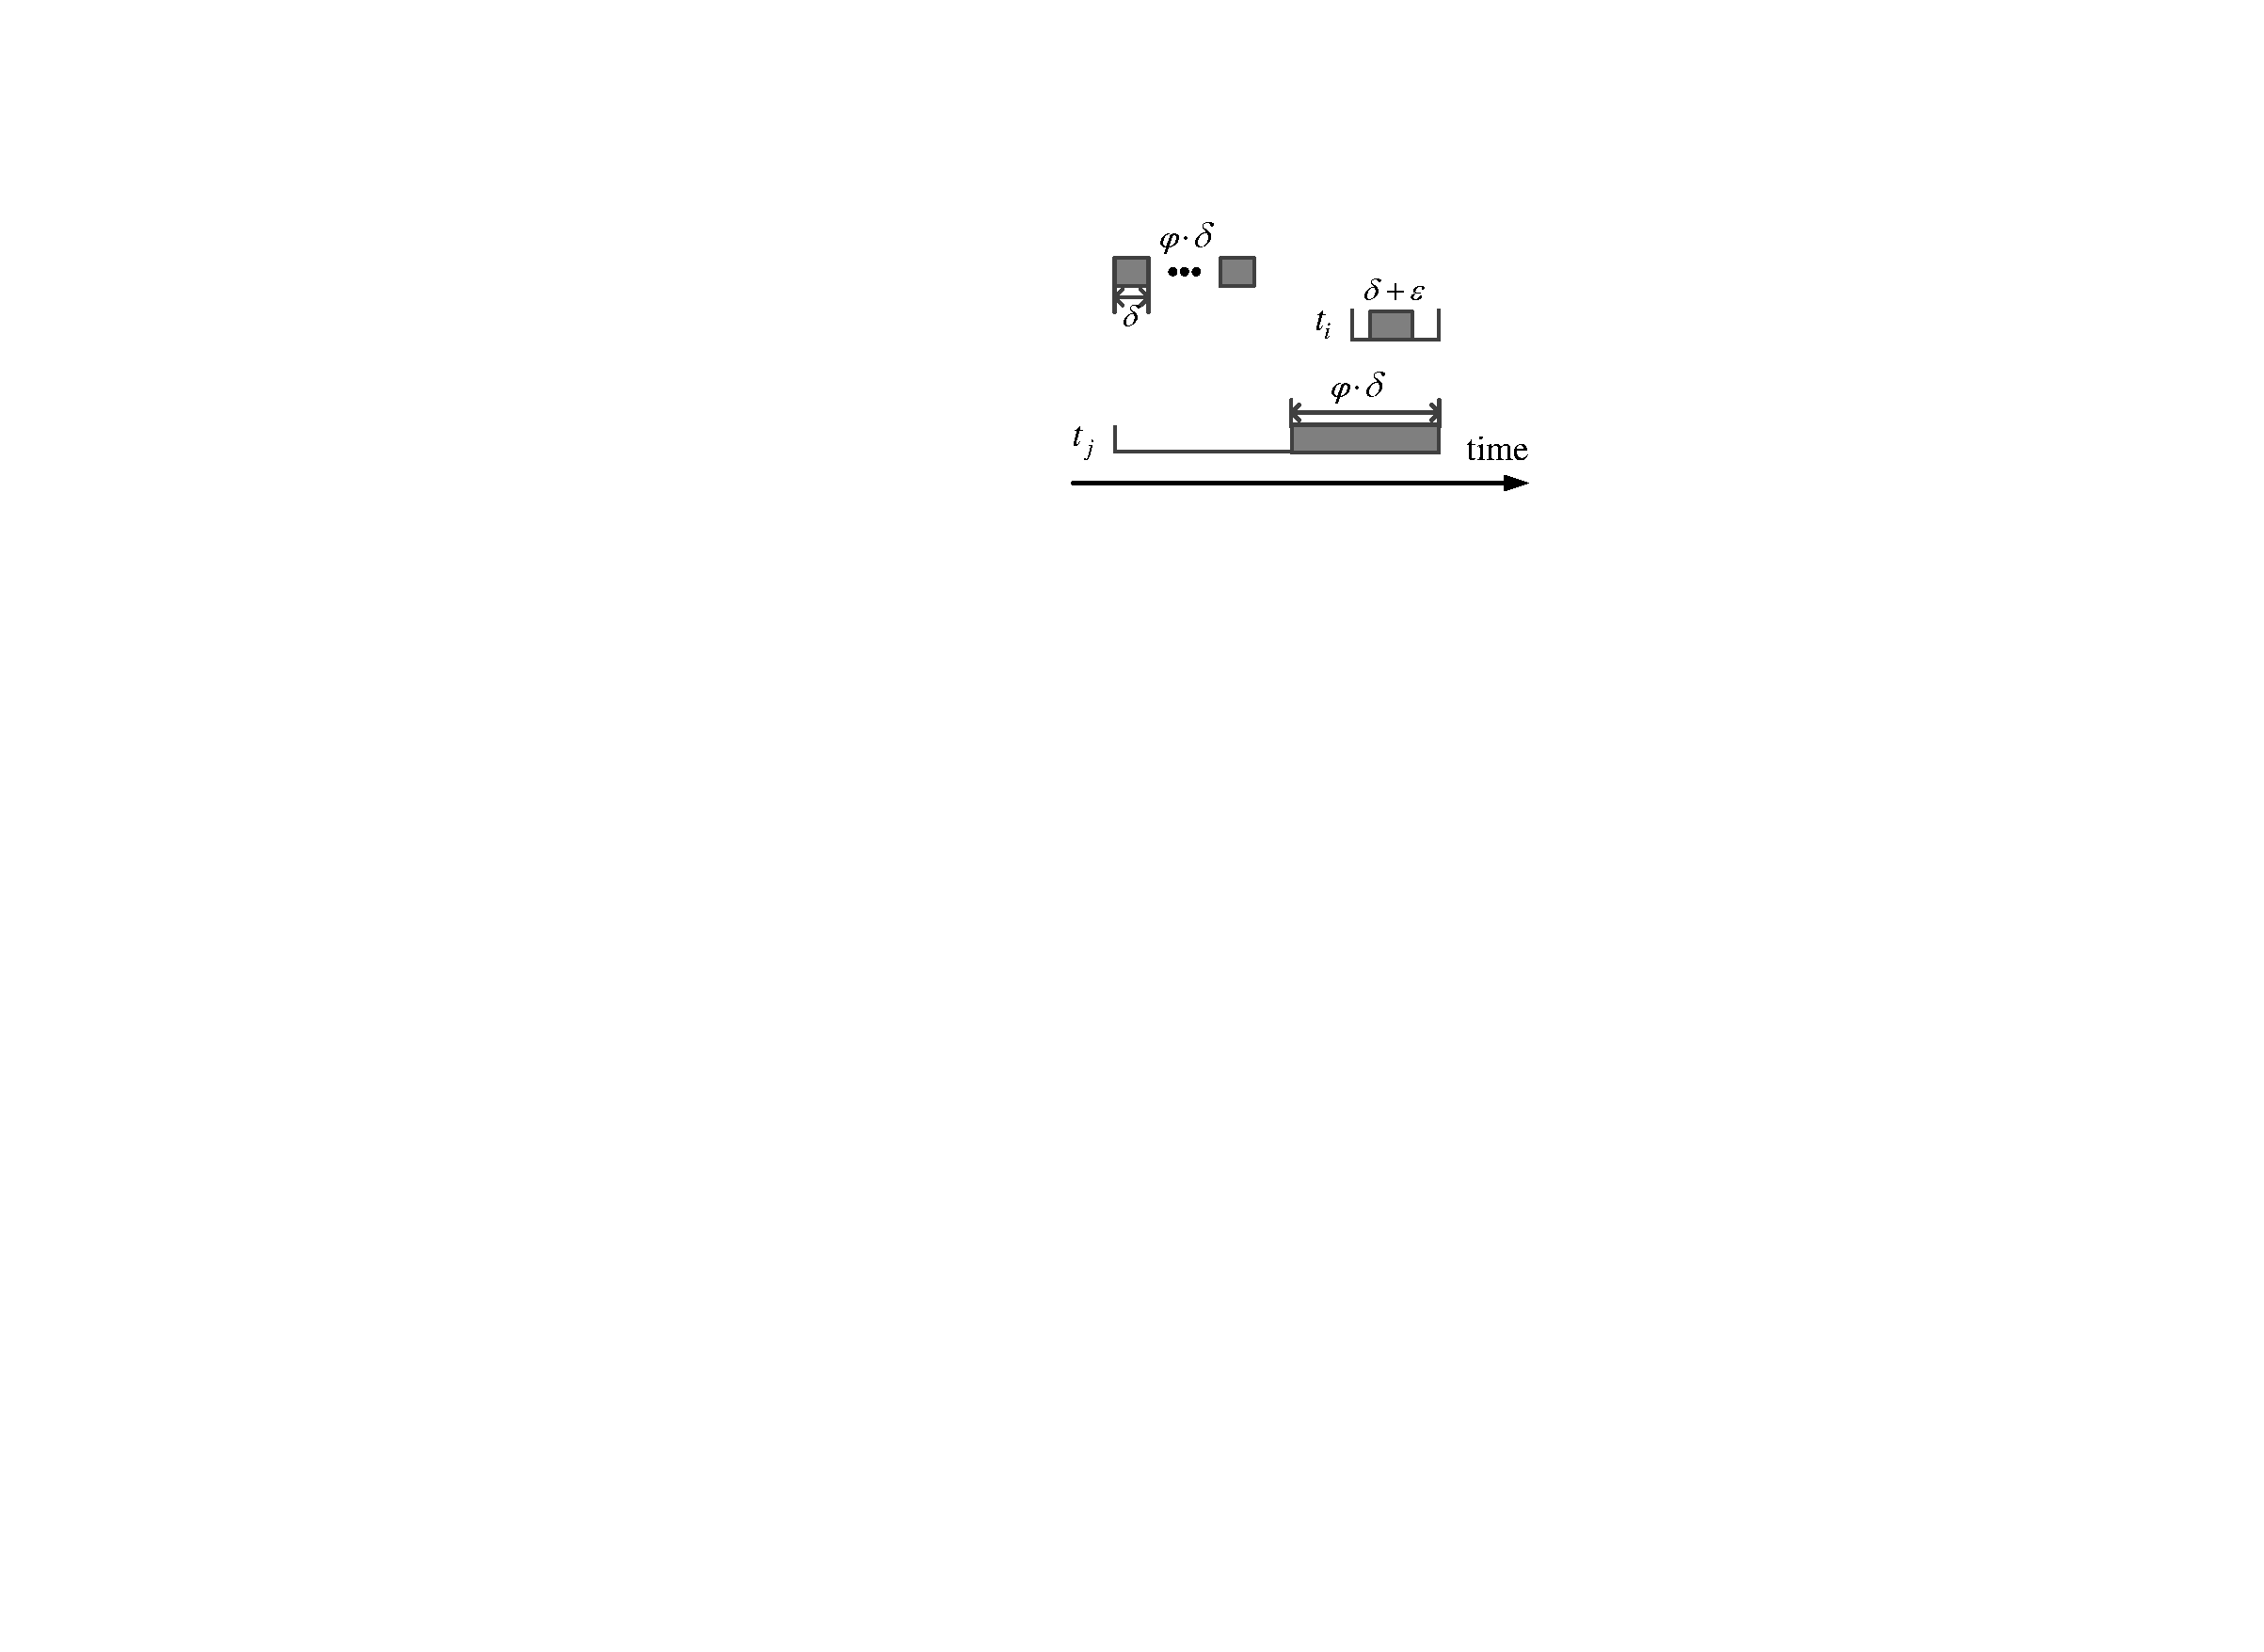
\includegraphics[width=0.46\columnwidth]{Figures/figure3_c}\label{figure3_c}}
%\subfigure[Optimal result]{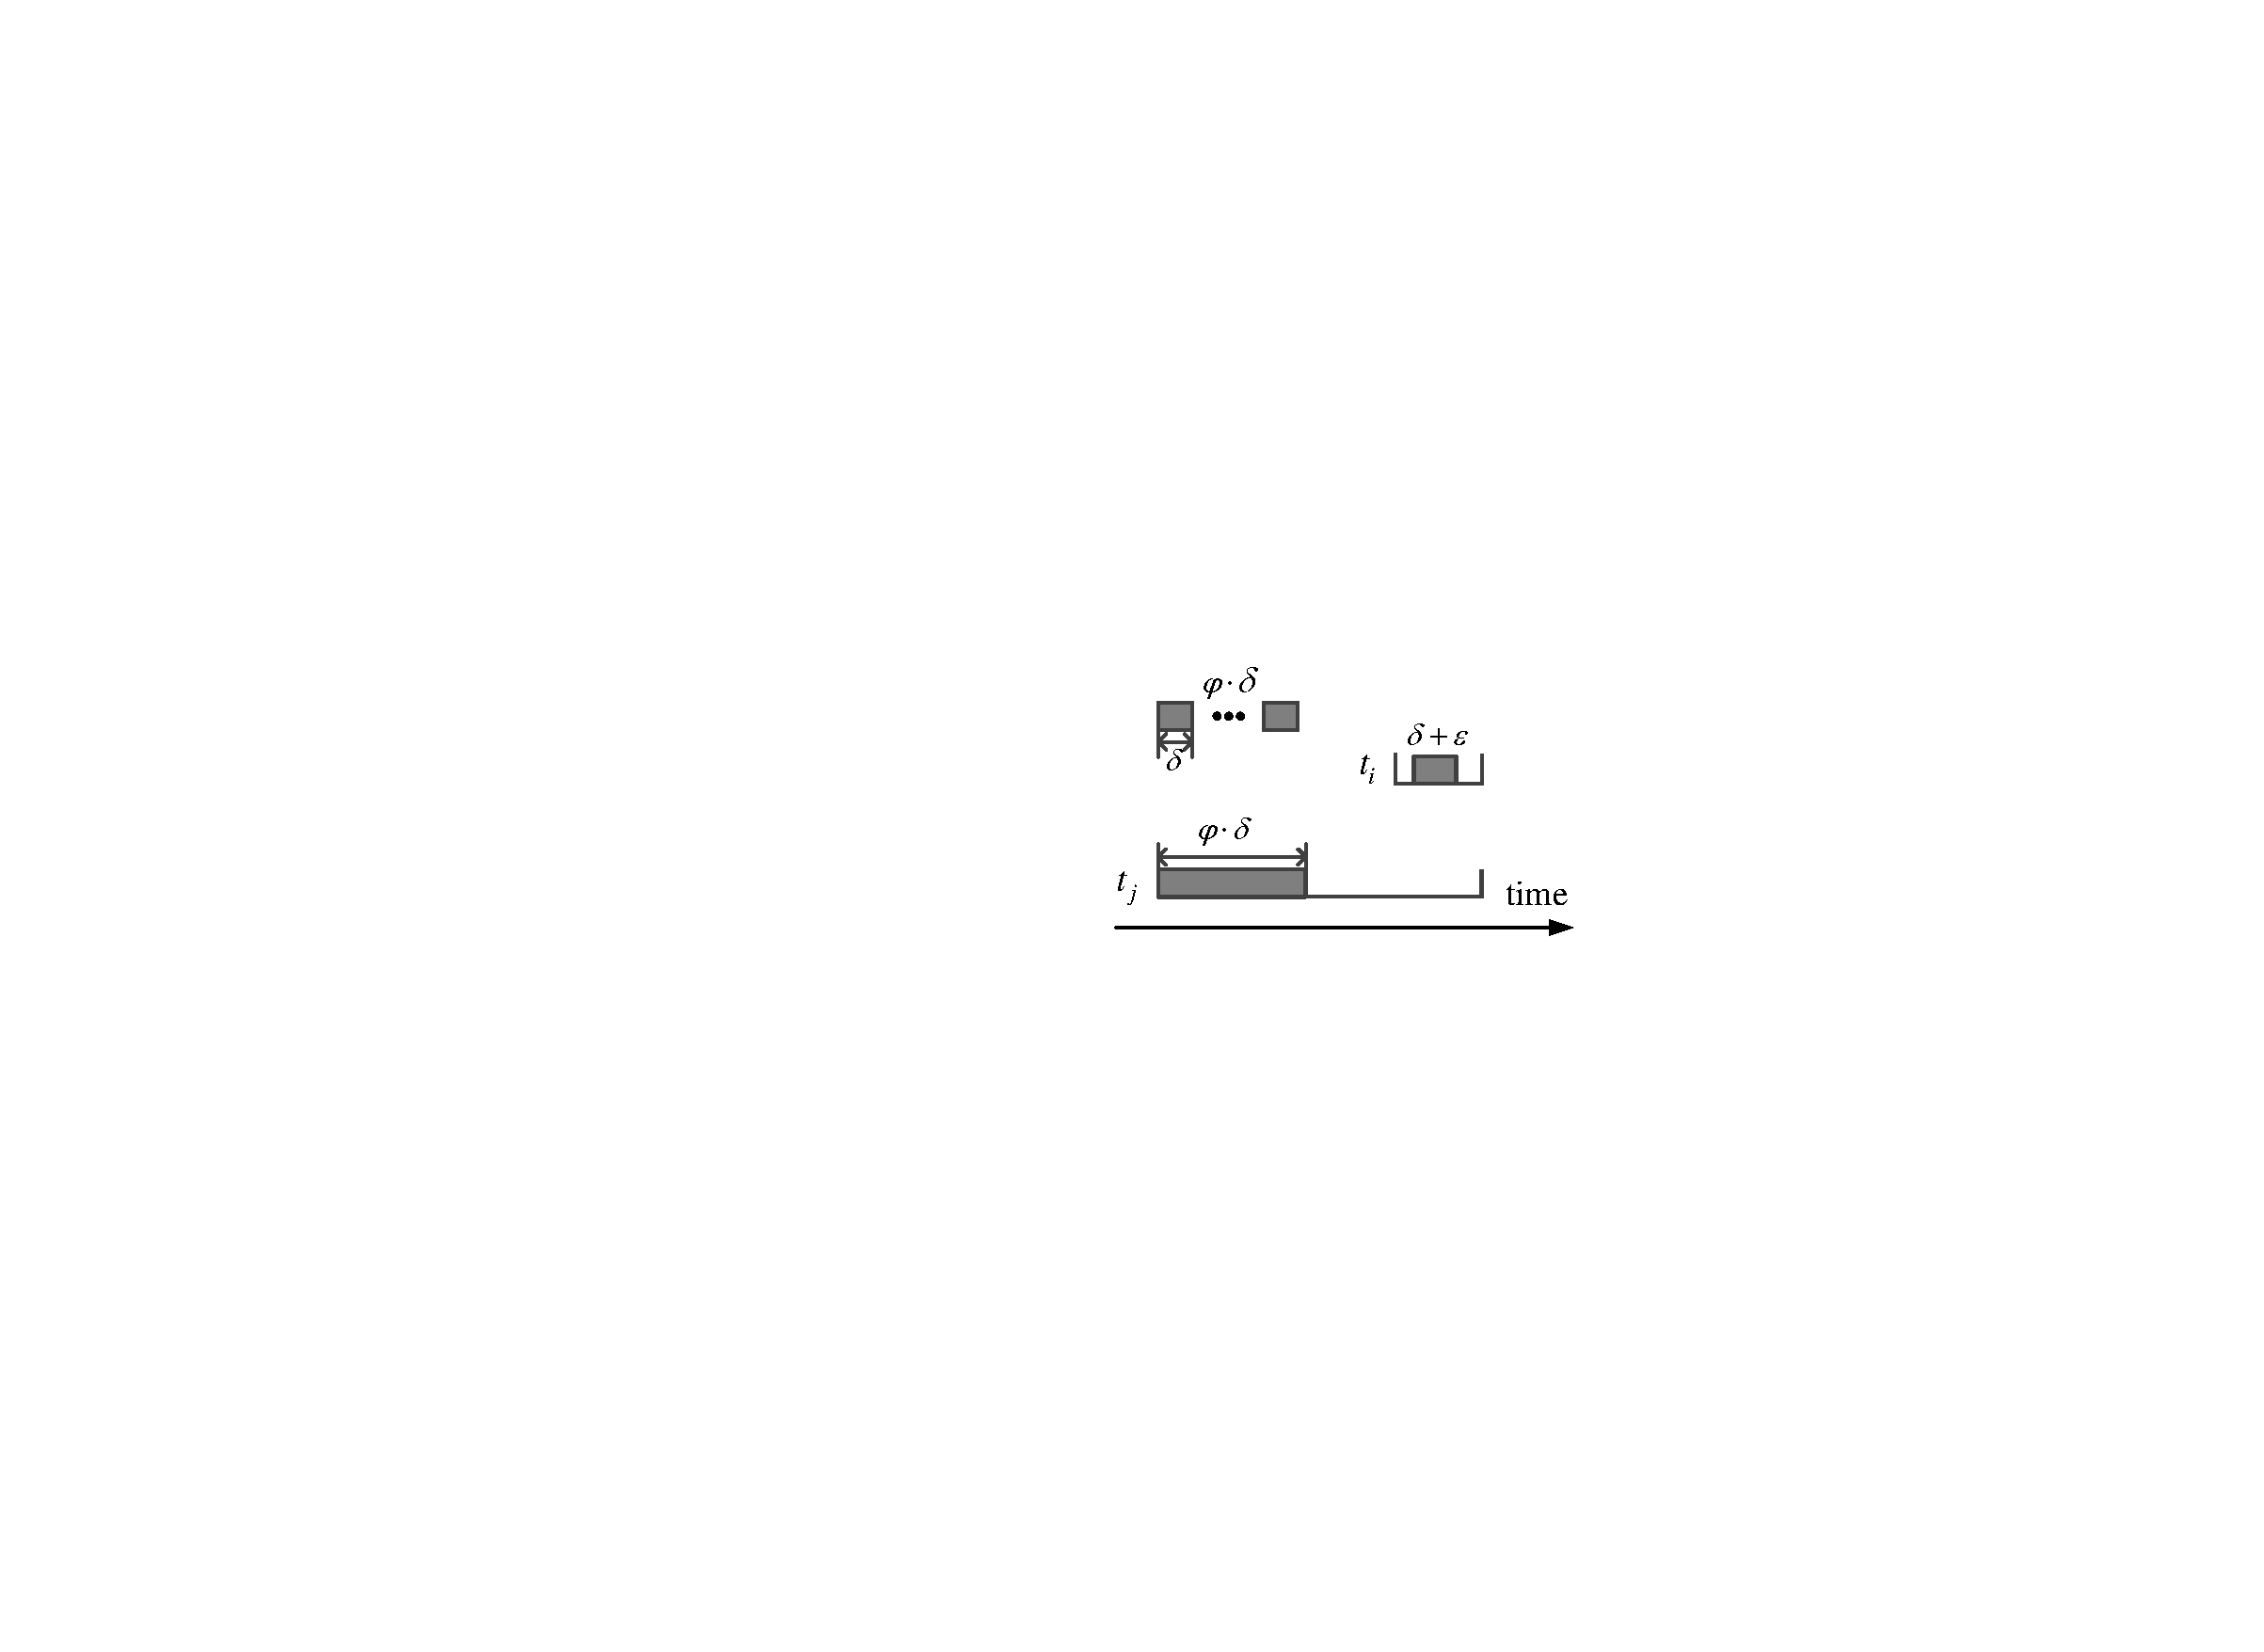
\includegraphics[width=0.46\columnwidth]{Figures/figure3_d}\label{figure3_d}}
%\caption{A typical example of the approximate result vs. the optimal result by using Algorithm \ref{algorithm_combine}.}
%\label{figure3_tight_example}
%\end{figure}
%
%As shown in Fig. \ref{figure_proof_scheduling_origin}, if the current candidate task pair is $\mathrm{<}t_i,t_j\mathrm{>}$, A task set is notated as $T'\mathrm{=}\{t_k\}$. $T'$, as indicated in Fig. \ref{figure_proof_scheduling_model}, can be presented as a compact model which at most consists of $\theta$ compact tasks. Here, $\delta$ is set to be smaller than $d(t_i,t_j)$. These compact tasks are placed along the time axis in the order of time. $\forall t\mathrm{\in} T'$, it does not overlap with $t_i$. Note that $\mathrm{<}t_i,t_j\mathrm{>}$ has the maximal overlap value for the current combination in $T$ and the compact model keeps the property.




\begin{theorem}
Algorithm \ref{algorithm_combine} is a 2-factor approximation scheduling algorithm.
\label{theorem_schedule}
\end{theorem}

\begin{proof}
For a non-empty task set $T$, if $|T|\mathrm{=}1$,  Algorithm \ref{algorithm_combine} returns the only one sampling task which is the optimal result.

When $|T|\mathrm{>} 1$, assume $I_i$ and $I_j$ are  the corresponding sampling intervals of tasks $t_i$ and $t_j$, respectively. $t_i$ and $t_j$ are overlapping.  $I$ is the sampling interval of a task set notated as $T'$ and $T'\mathrm{=}T\mathrm{-}\{t_i,t_j\}$. Considering the task $t_i$, in the worst case,  Algorithm \ref{algorithm_combine}  returns the resultant interval length  $|I_i \mathrm{\uplus} I_j \mathrm{\uplus} I|$ as illustrated in Fig. \ref{figure3_c}. However, there exists an optimal algorithm which derives the resultant interval length $|I_i \mathrm{\uplus} I|$ as illustrated in Fig. \ref{figure3_d}. Therefore, we have:
\begin{equation}
\begin{array}{lcl}
\frac{\displaystyle GREEDY(T)}{\displaystyle OPT(T)}&=&\frac{\displaystyle |I_i \uplus I_j \uplus I|}{\displaystyle |I_i \uplus I|}\\
       &=&\frac{\displaystyle \theta \cdot \delta+|I_i \uplus I_j|}{\displaystyle \theta \cdot \delta+|I_i|}\\
       &\le&1+\frac{\displaystyle |I_j|}{\displaystyle \theta \cdot \delta+|I_i|}\\
       &\le&1+\frac{\displaystyle \theta \cdot \delta}{\displaystyle \theta \cdot \delta+\delta}\\
       &\le&2.
\end{array}
\end{equation}
Here, $\delta \mathrm{\le}d(t_i,t_j)$.
\end{proof}

\begin{figure}
\centering
\subfigure[Greedy result]{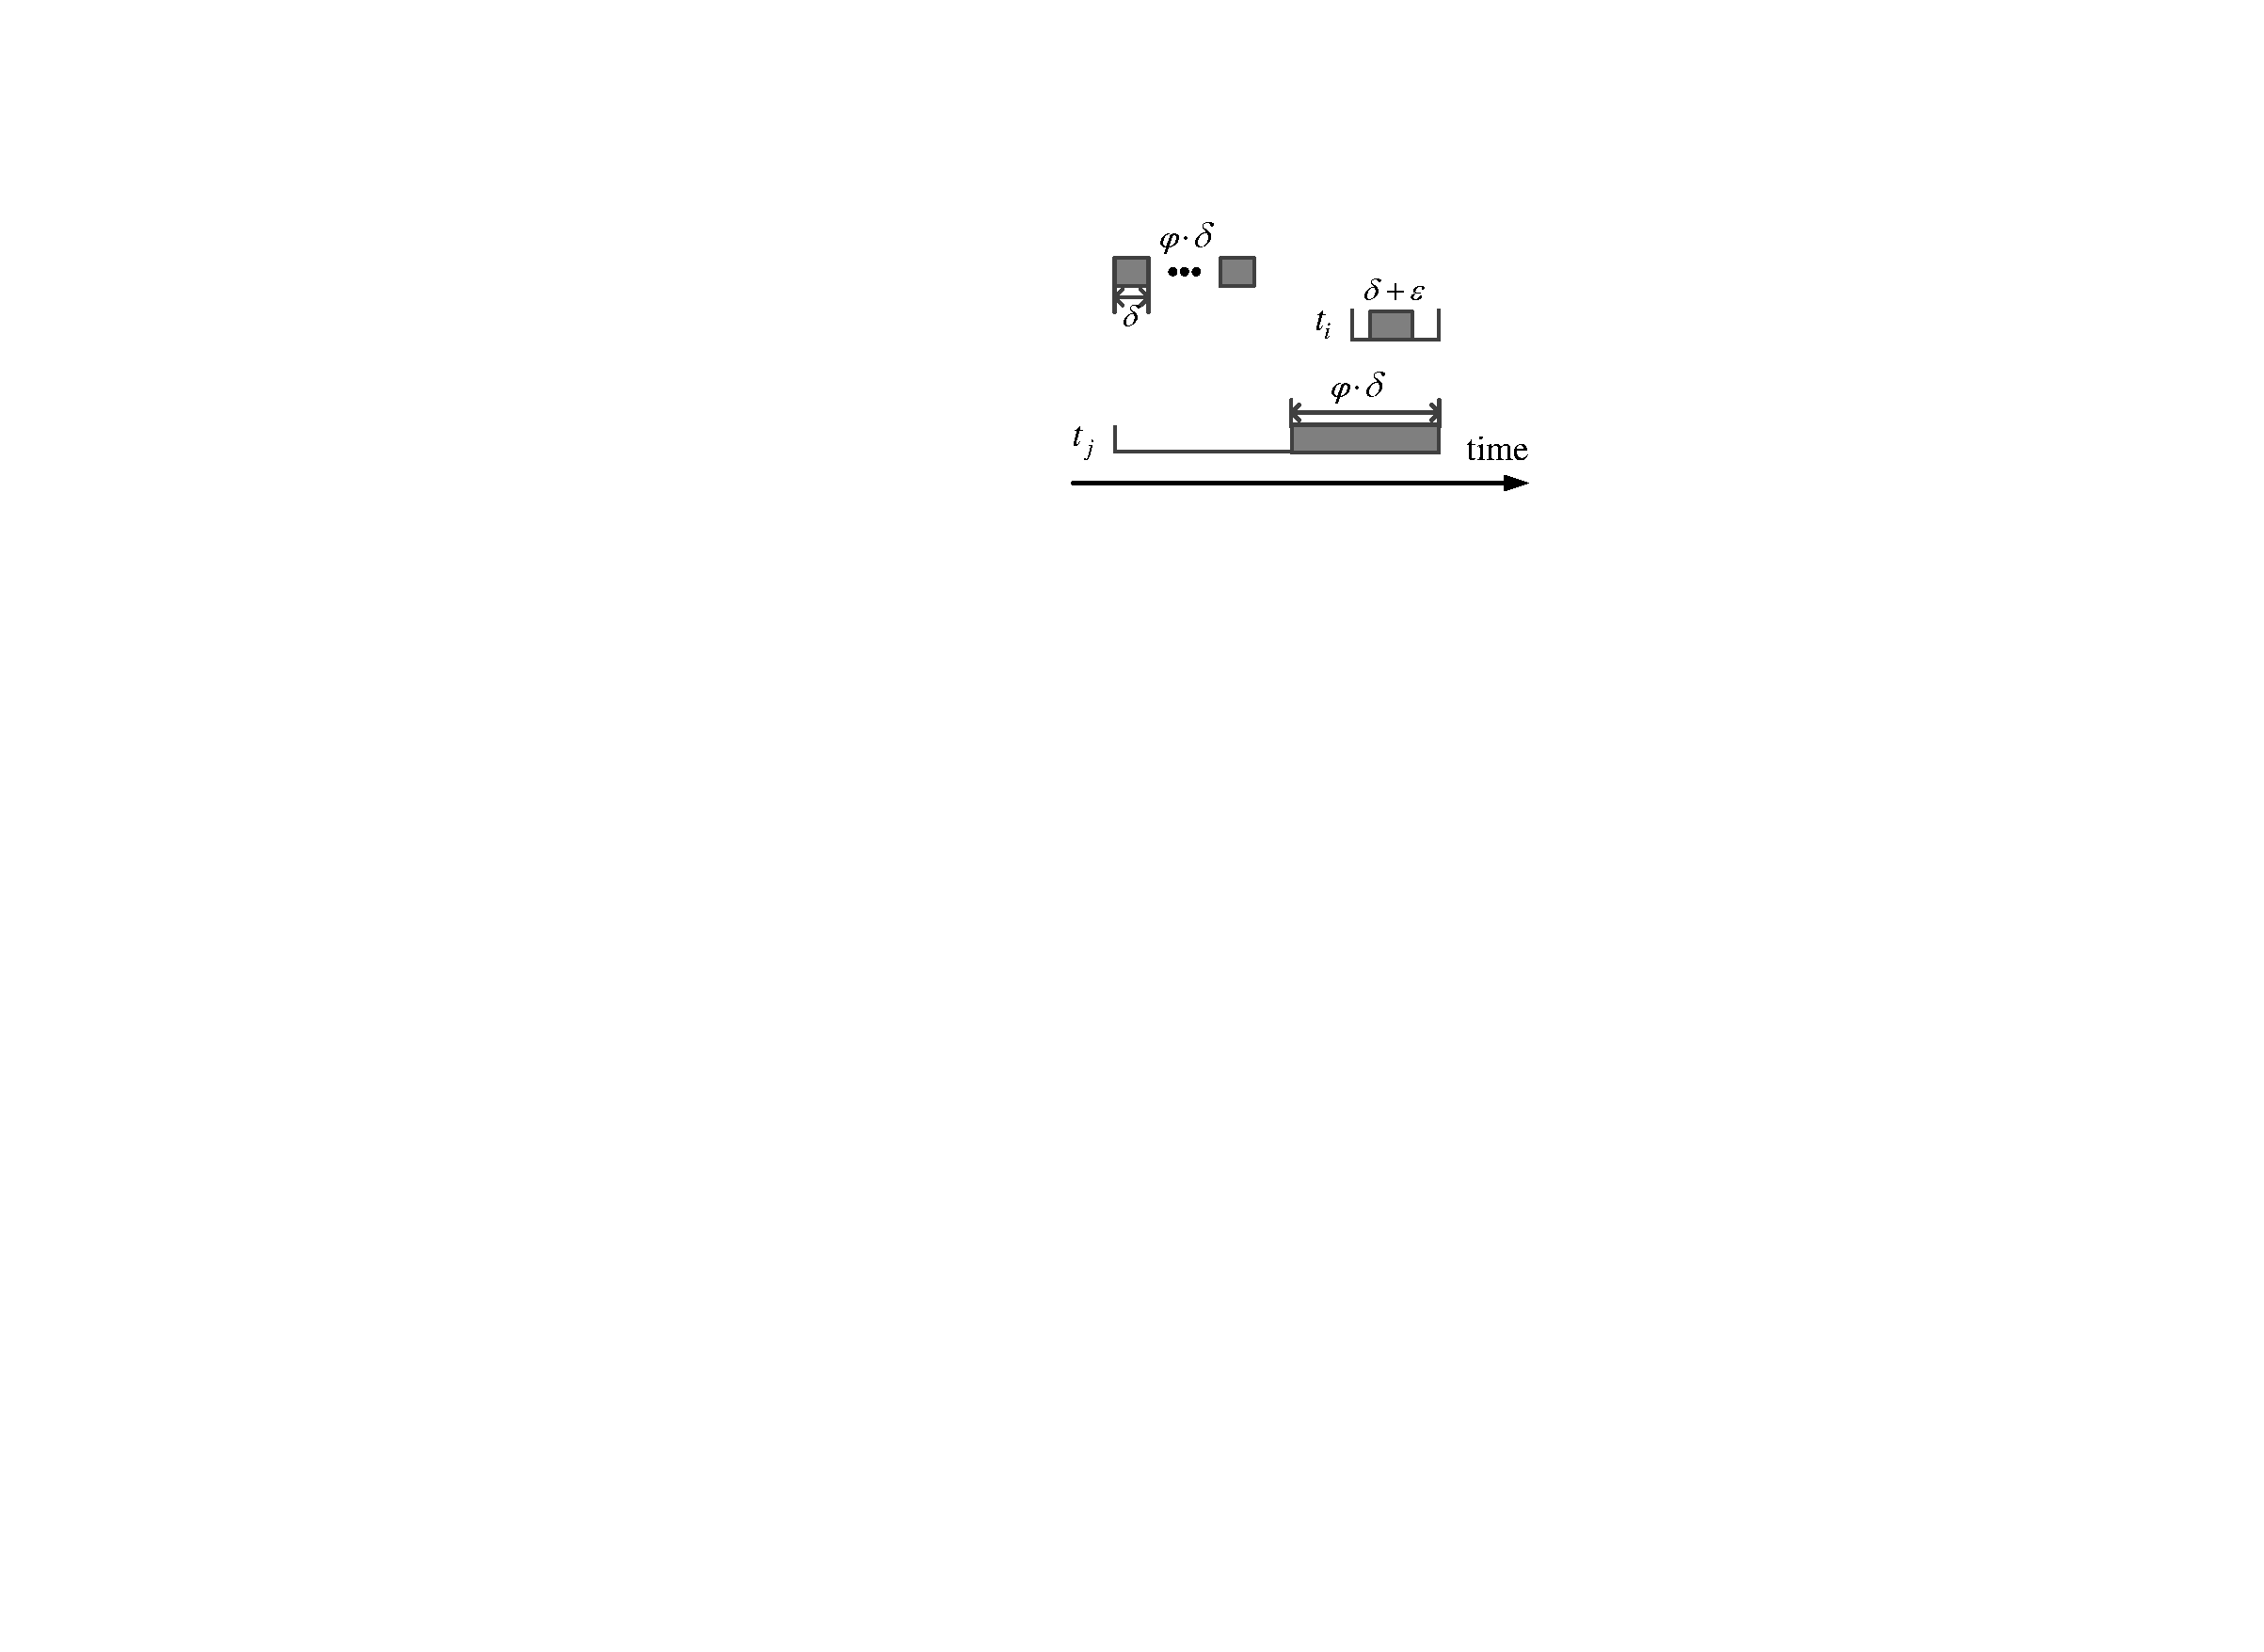
\includegraphics[width=0.26\columnwidth]{Figures/figure3_c}\label{figure3_c}}
\hspace{3pt}
\subfigure[Optimal result]{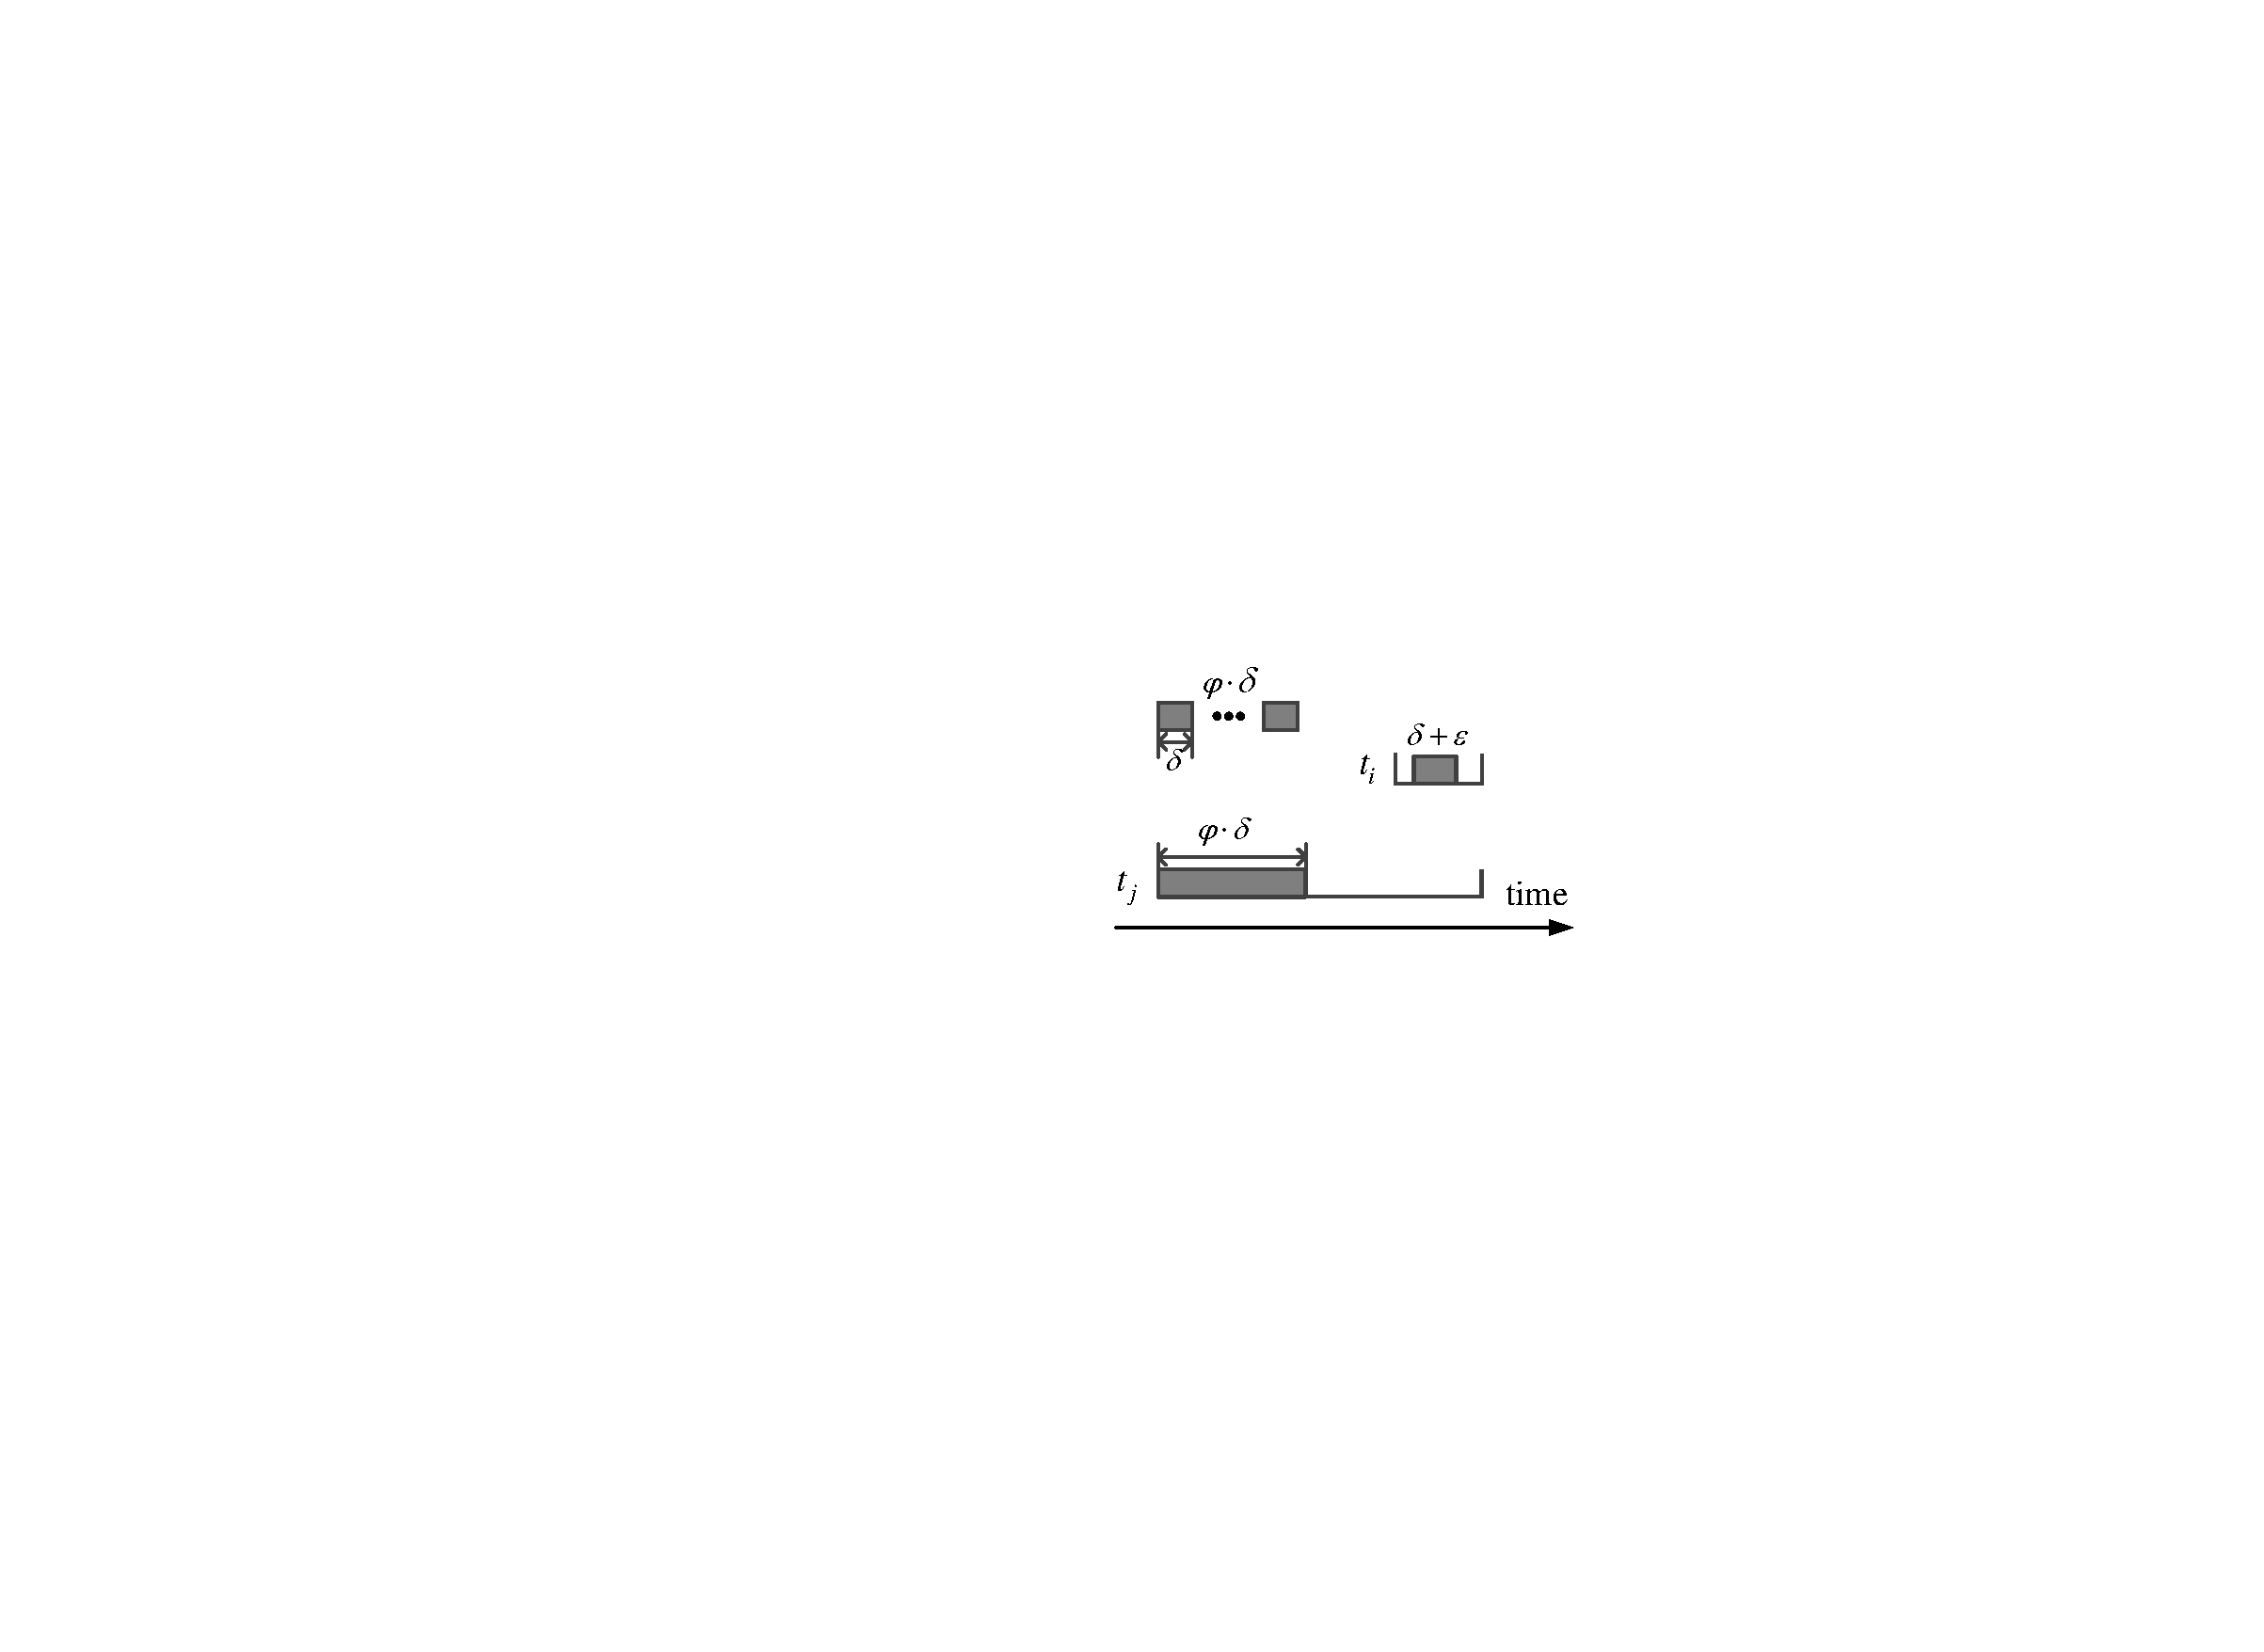
\includegraphics[width=0.26\columnwidth]{Figures/figure3_d}\label{figure3_d}}
\caption{A typical example of the approximate result by using Algorithm \ref{algorithm_combine} vs. the optimal result.}
\label{figure3_tight_example}
\end{figure}
%\begin{algorithm}[t]
%    \caption{Allocation\_Random$(T,S,k,r)$}
%    \label{allocation_random}
%    \begin{algorithmic}[1]
%        \Require A task set $T$ and $T\mathrm{\neq}\emptyset$. A sensor node set $S$ and $S\mathrm{\neq}\emptyset$. The task subset of a sensor node $t_i$ is denoted by $T_i$ with $T_i\mathrm{=}\emptyset$. $1\mathrm{\le} i \mathrm{\le} m$, $r\mathrm{\le} k$.
%        \While {$T \mathrm{\neq} \emptyset$}
%            \State randomly allocate a task $t$, $t \mathrm{\in} T$ to one of $k$ candidate sensor nodes $s_i$  which do not have been allocated $t$ before.
%            \State $T_i \leftarrow T_i \bigcup \{t\}$.
%            \State $t.count\mathrm{=}t.count\mathrm{+}1$.
%            \If {$t.count\mathrm{==} r$}
%                \State remove $t$ form $T$.
%            \EndIf
%        \EndWhile
%        \State \textbf{Combine($T_i$)} for each task subset $T_i$.
%    \end{algorithmic}
%\end{algorithm}


A typical example is shown in Fig. \ref{figure3_tight_example}. Algorithm \ref{algorithm_combine} returns the interval length $2 \theta\mathrm{\cdot} \delta$ where $\delta \mathrm{<} d(t_i,t_j)$, while the optimal result is $\theta \mathrm{\cdot} \delta\mathrm{+}\varepsilon$. Thus:
%\vspace{-2pt}
\begin{equation}
 \lim \limits_{\varepsilon \mathrm{\to} 0, \theta \mathrm{\to} \infty} \frac{\theta \mathrm{\cdot} \delta \mathrm{+} \theta \mathrm{\cdot} \delta}{\theta \mathrm{\cdot} \delta \mathrm{+}\delta\mathrm{+} \varepsilon}\mathrm{=}2.
 \vspace{0pt}
\end{equation}

Our algorithm performs better when a task is  overlapping with others tightly. Experimental results in Section \ref{section_evaluation} have verified this viewpoint.

\section{A 2-factor approximation allocation algorithm designing for WSNs}

\label{section_allocation}
In this section, we provide three algorithms for the task allocation problem. The first is a random algorithm which allocates the sampling tasks randomly. The second is a pruning algorithm which first allocates a task to all candidate nodes and then removes it from some of the candidate sensor nodes by its overlap value with other tasks.  The third is a $2$-factor approximation algorithm which allocates sampling tasks by iteratively combining them until no overlapping tasks exist.

For any task set, the insight of the random allocation method is to randomly identify $r$ out of $k$ candidate sensor nodes. This method is simple and easy to be performed on a sensor node. However, it ignores the overlap amongst the tasks and  brings much unnecessary sampled data which consumes much energy of sensor nodes and damages the quality of communication in WSNs as well.

\subsection{Task allocation according to the pruning operation}

\begin{algorithm}[t]
	\SetAlgoNoLine
	\KwIn{A task set $T$ and $T\mathrm{\neq}\emptyset$. A sensor node set $S$ and $S\mathrm{\neq}\emptyset$. $1\mathrm{\le} i \mathrm{\le} m$. $r\mathrm{\le} k$.}
	\KwOut{A task set where there are no overlapping tasks.}
    \caption{Allocation\_Prune}
    \label{allocation_prune}
    %\begin{algorithmic}[1]
        \Repeat {$T \mathrm{\neq} \emptyset$}{
            allocate a task $t$, $t \mathrm{\in} T$  to $k$ candidate sensor nodes\;
            compute the value of  data sharing $d(t,\cdot)$ between $t$ and any other tasks on a sensor node\;
            \eIf {no sampling task is overlapping with $t$}
                {randomly allocate $t$ to one candidate sensor node\;}
                {remove the task $t$ from a candidate sensor node when $t$ has the smallest value of data sharing  with other  tasks on the node\;}
            $t.count\mathrm{=}t.count\mathrm{-}1$\;
            \If {$t.count\mathrm{==} r$}
                {remove $t$ from $T$\;}
        }
        \textbf{Combine} for each task subset $T_i$\;
    %\end{algorithmic}
\end{algorithm}


We notice that the sampled data can be shared in the overlapping time region. Therefore, we consider allocating tasks via the pruning operation which removes unreasonable allocation choices repeatedly. The entire process contains three major steps. First, we allocate tasks to all candidate sensor nodes. That is, if a task is detected by $k$ sensor nodes, it is allocated to all the $k$ candidate sensor nodes. Second, compute the maximal overlap value between a task and other overlapping tasks. Then remove a task from a sensor node where the task has the smallest overlap value with other tasks until it is allocated to $r$ sensor nodes. Finally, compute the total length of sampling intervals. Algorithm \ref{allocation_prune} describes more details.

%\begin{figure}[t]
%\centering
%\subfigure[The approximate result of task allocation by using the Algorithm \ref{allocation_prune}.]{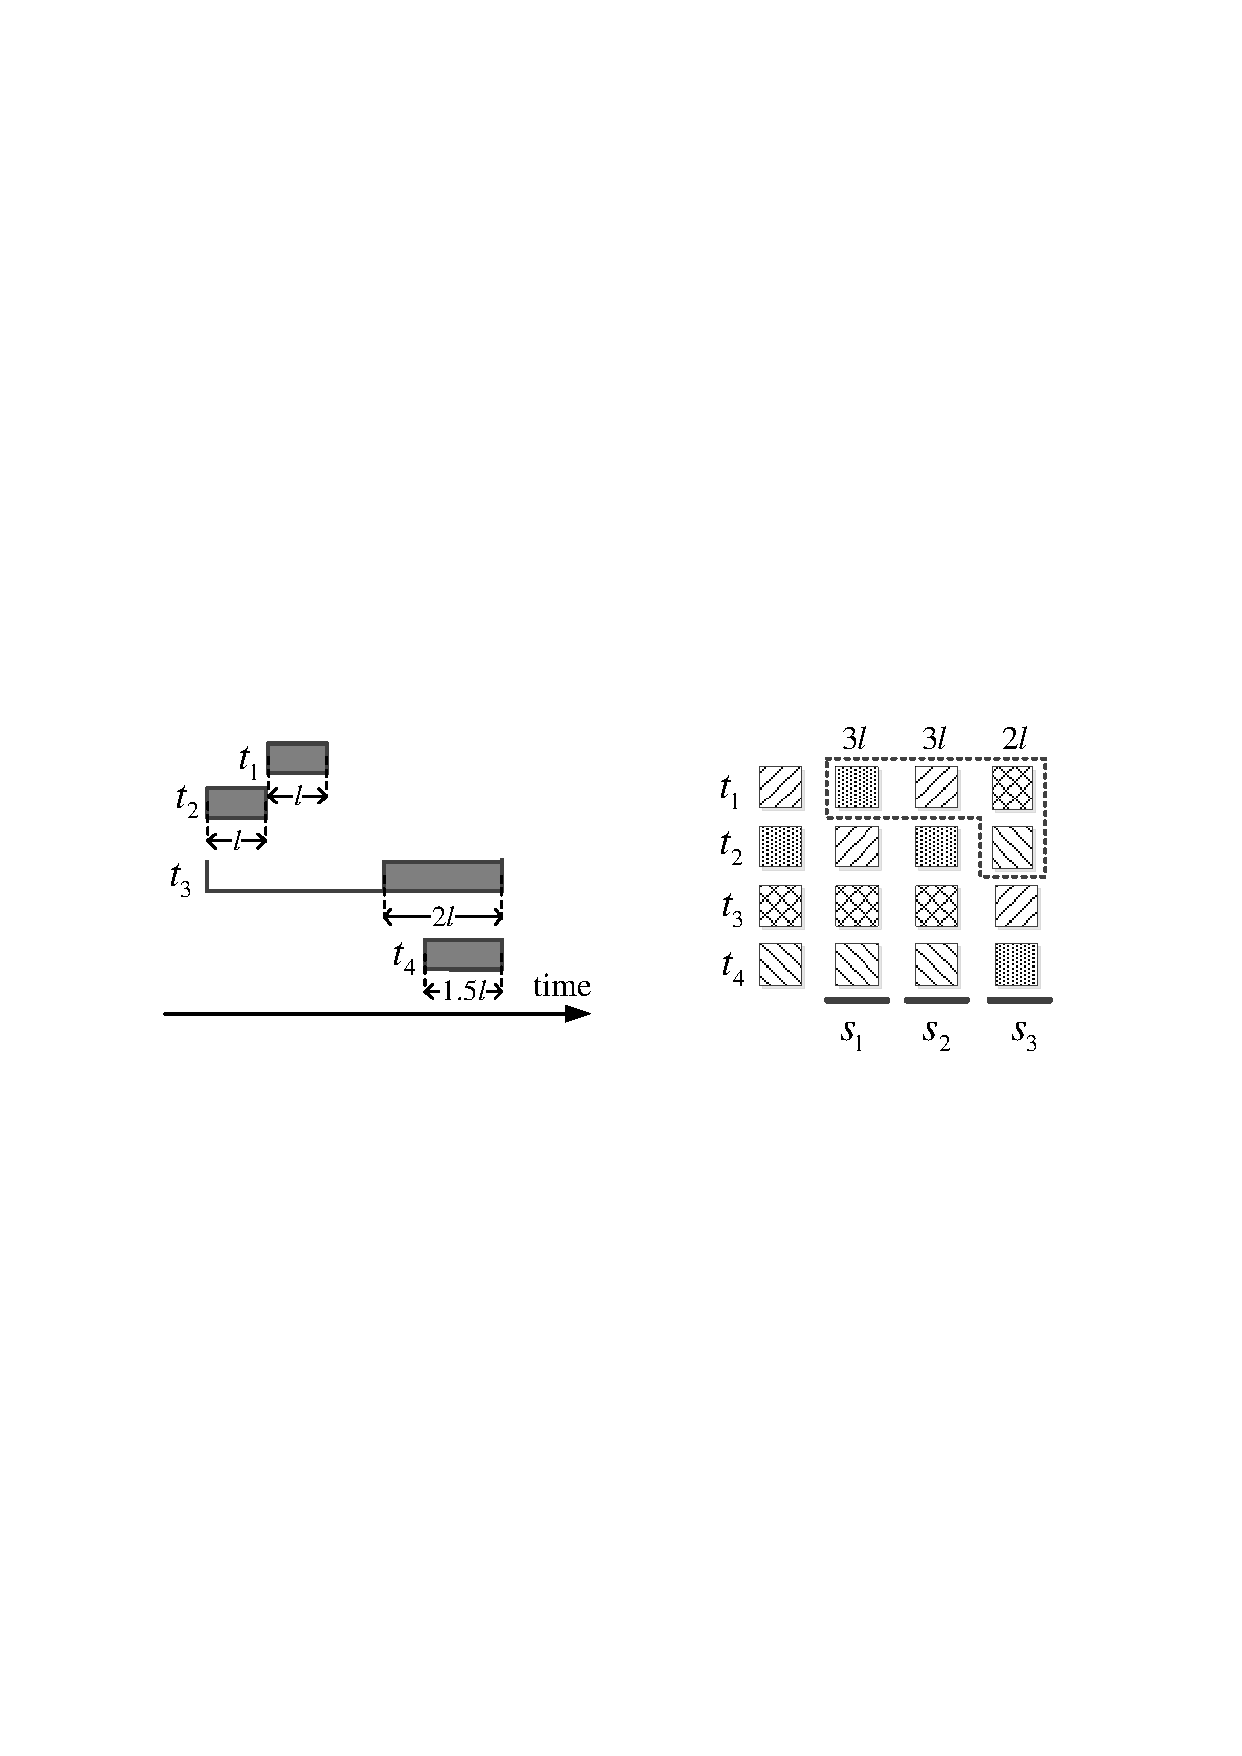
\includegraphics[width=0.9\columnwidth]{Figures/figure_prune_allocation_1}\label{figure_prune_allocation_1}}
%\subfigure[The optimal result of task allocation by using the Algorithm \ref{allocation_prune}.]{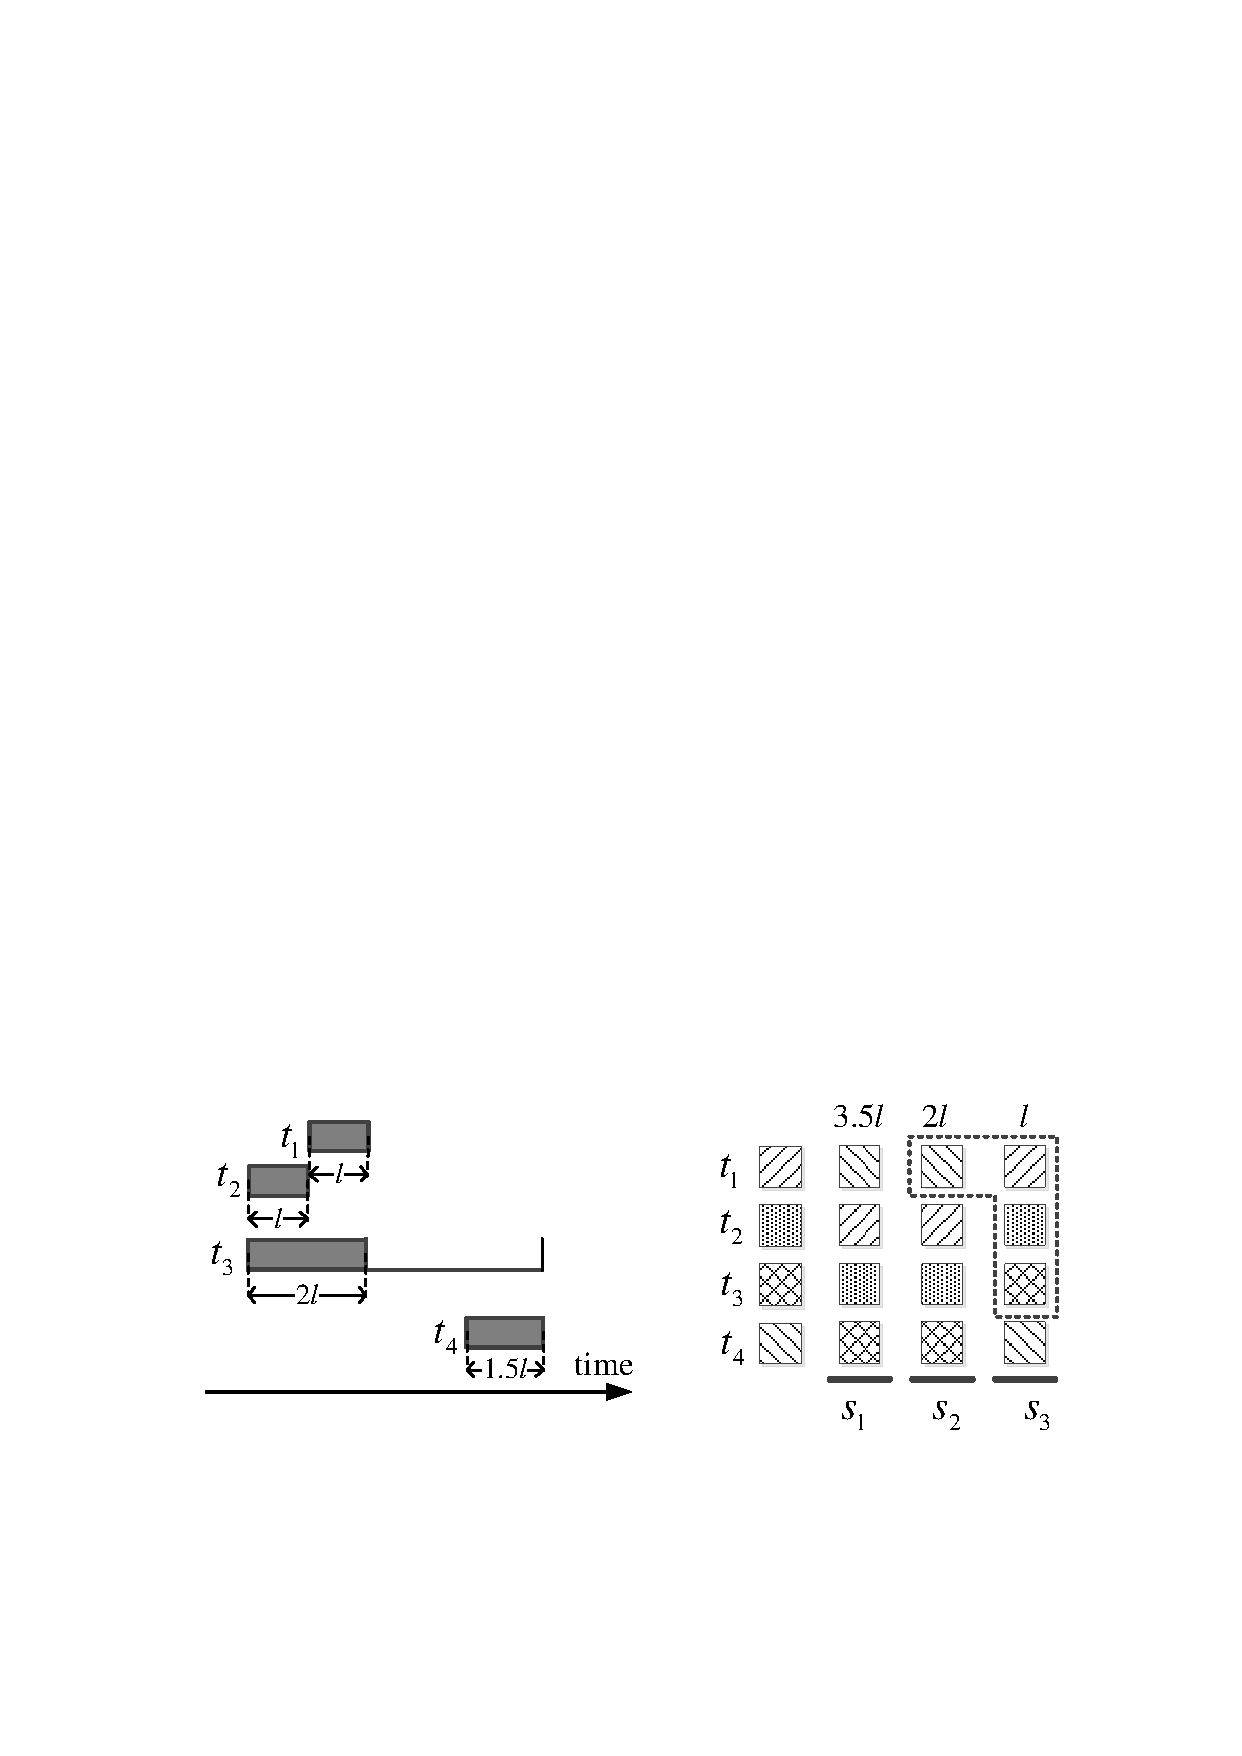
\includegraphics[width=0.9\columnwidth]{Figures/figure_prune_allocation_2}\label{figure_prune_allocation_2}}
%%\renewcommand{\figurename}{abc}
%\caption{A typical example of the approximate result vs. the optimal result by using Algorithm \ref{allocation_prune}. The four tasks in the left are represented as four colors in the right, respectively.  The tasks in the dotted rectangular will be removed from the nodes in the pruning procedure.}.
%\label{figure_prune_example}
%\end{figure}
\begin{figure}[t]
\centering
\subfigure[The approximate result of task allocation by using Algorithm \ref{allocation_prune}.]{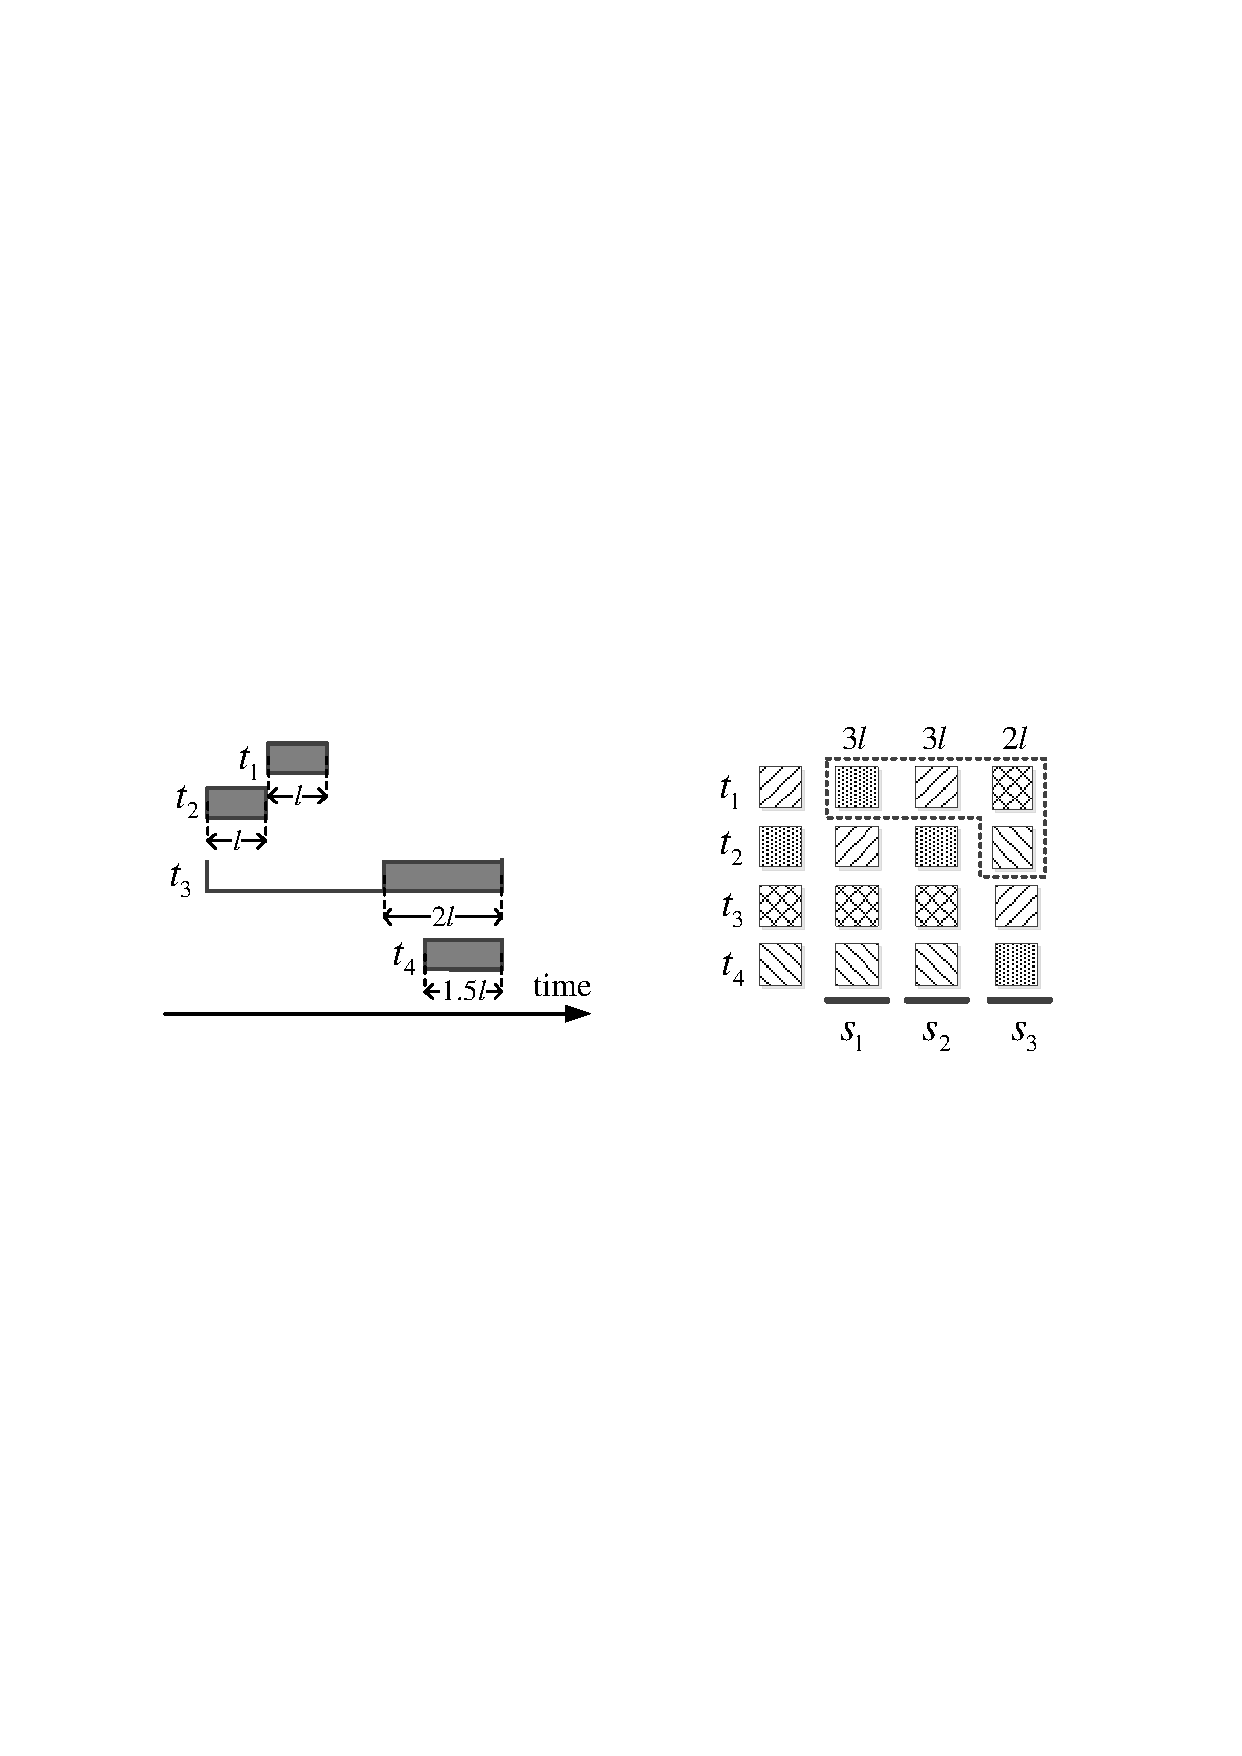
\includegraphics[width=0.47\columnwidth]{Figures/figure_prune_allocation_1}\label{figure_prune_allocation_1}}
\subfigure[The optimal result of task allocation.]{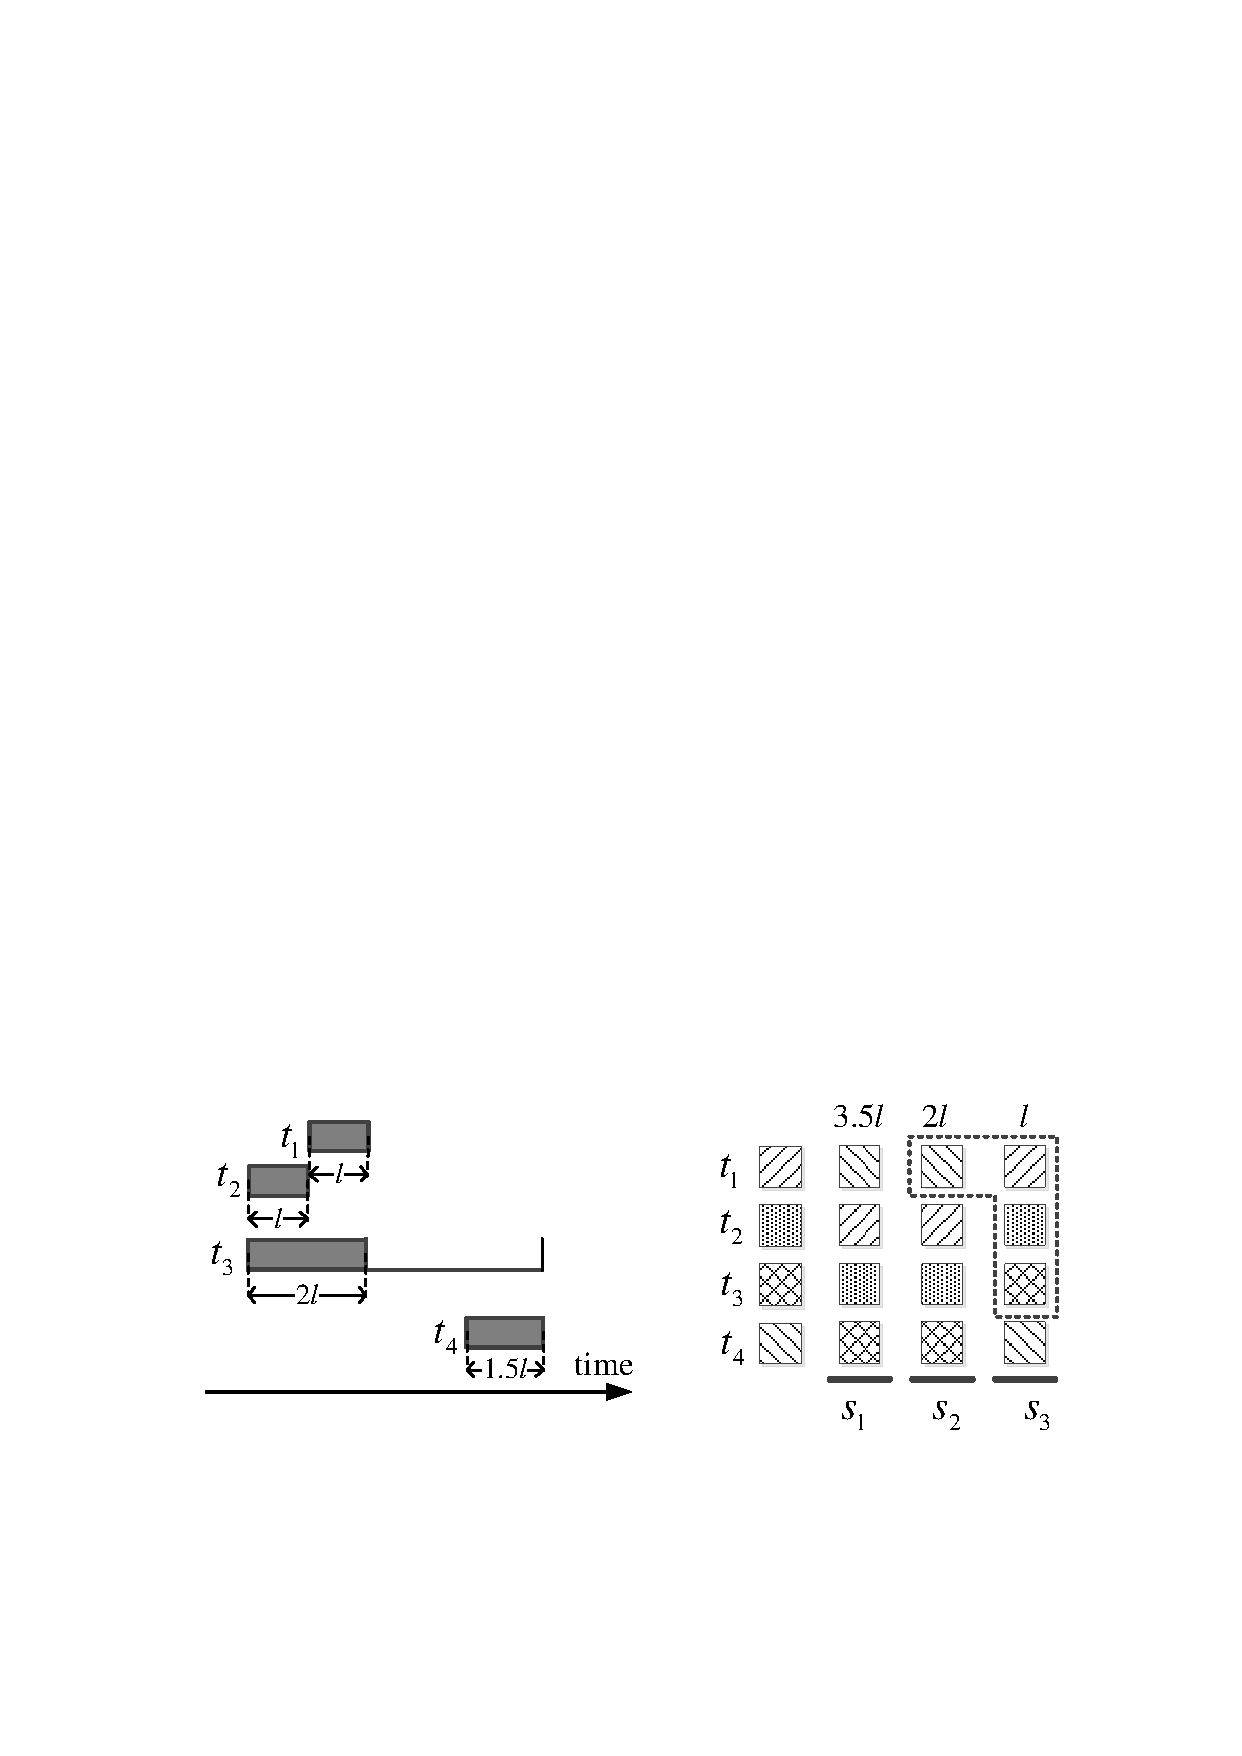
\includegraphics[width=0.47\columnwidth]{Figures/figure_prune_allocation_2}\label{figure_prune_allocation_2}}
%\renewcommand{\figurename}{abc}
\caption{A typical example of the approximate result by using Algorithm \ref{allocation_prune} vs. the optimal result.  Tasks in the dotted polygon will be removed from nodes due to pruning operations.}.
\label{figure_prune_example}
\end{figure}

In Algorithm \ref{allocation_prune}, lines $2\mathrm{-}3$ allocate a task to its $k$ candidate sensor nodes.  Lines $4\mathrm{-}8$ check whether a task has been removed from $k\mathrm{-}r$ candidate sensor nodes. Line $11$ computes the final sampled data for each sensor node using Algorithm \ref{algorithm_combine}. In the worst case, if Algorithm \ref{algorithm_combine} is used to compute the sampled data, the time complexity of Algorithm \ref{allocation_prune} is $O(n^2)$, and the space complexity is $O(n^2)$. If Algorithm \ref{algorithm_combine2} is used to compute the sampling time, then the space complexity of Algorithm \ref{allocation_prune} is $O(k\cdot n/m)$ because each task maintains its $k$ maximal overlap value for all candidate sensor nodes.

Algorithm \ref{allocation_prune} is a greedy algorithm. A typical  example is shown in Fig. \ref{figure_prune_example}. Here, $k\mathrm{=}3$ and $r\mathrm{=}2$. The sensor node set is notated as $S$ where $S\mathrm{=}\{s_1,s_2,s_3\}$. The task set is notated as $T$ and $T\mathrm{=}\{t_1,t_2,t_3,t_4\}$. As illustrated in Fig. \ref{figure_prune_example}, we use four different types of rectangles in the right to stand for the tasks in the left. The pruning allocation method first allocates all the sampling tasks to the candidate nodes, and then removes the tasks which has smaller overlap with other tasks (indicated in dotted rectangular). Finally, Algorithm \ref{allocation_prune} returns the total length of sampling intervals $8l$ as shown in Fig. \ref{figure_prune_allocation_1}, while the optimal result is $6.5l$ as shown in Fig. \ref{figure_prune_allocation_2}. The reason is that our pruning procedure is not optimal in each round. This motivates us to propose Algorithm \ref{allocation_combine} which allocates tasks according to the combination operation and can be optimal for each round.

\subsection{Tasks allocation according to the combination operation}

%\begin{table}[b]
%\centering
%\caption{Task allocation according to combination operation}
%\begin{tabular}{|c|c|c|c|
%c|c|c|c|c|}
%\hline
%    quad& $t_i$& $t_j$& $t$& $d(t_i,t_j)$& \multicolumn{4}{c|}{combination}\\ \hline
%    $q_{12}$& $t_1$& $t_2$& $\mathrm{<}0,4,4\mathrm{>}$&  $1$& & &   $\surd$&$\surd$\\ \hline
%    $q_{23}$& $t_2$& $t_3$& $\mathrm{<}3,8,4\mathrm{>}$&  $2$& &$\times$&&\\ \hline
%    $q_{24}$& $t_2$& $t_4$& $\mathrm{<}4,8,4\mathrm{>}$&  $2$& &$\times$&&\\ \hline
%    $q_{34}$& $t_3$& $t_4$& $\mathrm{<}4,8,4\mathrm{>}$&  $4$&$\surd$& $\surd$&&\\ \hline
%\end{tabular}
%\label{allocation_table}
%\end{table}

\begin{algorithm}[t]
	\SetAlgoNoLine
	\KwIn{A task set $T$ and $T \mathrm{\neq} \emptyset$. A sensor node set $S$ and $S \mathrm{\neq} \emptyset$. $r\mathrm{\le} k$, $|S|\mathbf{=}m$.}
	\KwOut{A task set where there are no overlapping tasks.}
    \caption{Allocation\_Combine}
    \label{allocation_combine}
    %\begin{algorithmic}[1]
        maintain a task set $T_i$ for the sensor node $s_i$\;
        $Q_i=$ Pre\_processing ($T_i$), and sort $Q_i$ in the descending order of the overlap value\;
        \Repeat {there exists overlapping tasks in $T_1,...,T_m$}{
            identify a task pair $\mathrm{<}t_1,t_2\mathrm{>}$ from $T_i$ which has the maximal overlap value\;
            combine $t_1$ and $t_2$ and notate the resultant task as $t$\;
            %\State remove $t_1$ and $t_2$, if they are in $T$;
            remove $t_1$ and $t_2$ from $T_i$\;
            add $t$ into $T_i$, and update $Q_i$\;
        }
        \Repeat {$T_i$ $(1\mathrm{\le} i\mathrm{\le} k)$ is not an empty set}{
            randomly allocate a task $t$ $(t\in T_i)$ to a sensor node which is not allocated $t$ before\;
            remove $t$ form $T_i$ if the task is allocated to $r$ out of $k$ sensor nodes\;
        }
        \textbf{Combine} for each task subset $T_i$\;
    %\end{algorithmic}
\end{algorithm}


The combination operation is utilized to schedule sampling tasks in Algorithm \ref{algorithm_combine}. Furthermore, the allocation problem can be solved by the combination operation. As illustrated in Fig. \ref{figure_overview}, a task $t$ is detected by three sensor nodes, but only two of them are identified to perform it. If the task $t$ is overlapping with three tasks $t_1$, $t_2$ and $t_3$ such that $d(t,t_1)\mathrm{>}d(t,t_2)\mathrm{>}o(t,t_3)$,  we should allocate $t$ to the sensor nodes $s_1$ and $s_2$.  The task allocation method includes three major operations. First, maintain a global quad list in which each quad stands for a combination operation of two overlapping tasks. Second, iteratively identify a quad which has the maximal overlap value of overlapping tasks in the global quad. Then allocate them to $r$  out of $k$ candidate sensor  nodes. Finally, update the quad list and the task set. Algorithm \ref{allocation_combine} presents the method of task allocation in detail.

\begin{figure}[t]
\centering
\subfigure[The first round of task combination.]{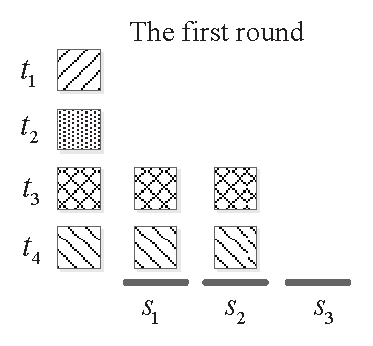
\includegraphics[width=0.22\columnwidth]{Figures/figure_combination_allocation_1}\label{figure_combination_allocation_1}}
\hspace{30pt}
\subfigure[The second round of task combination.]{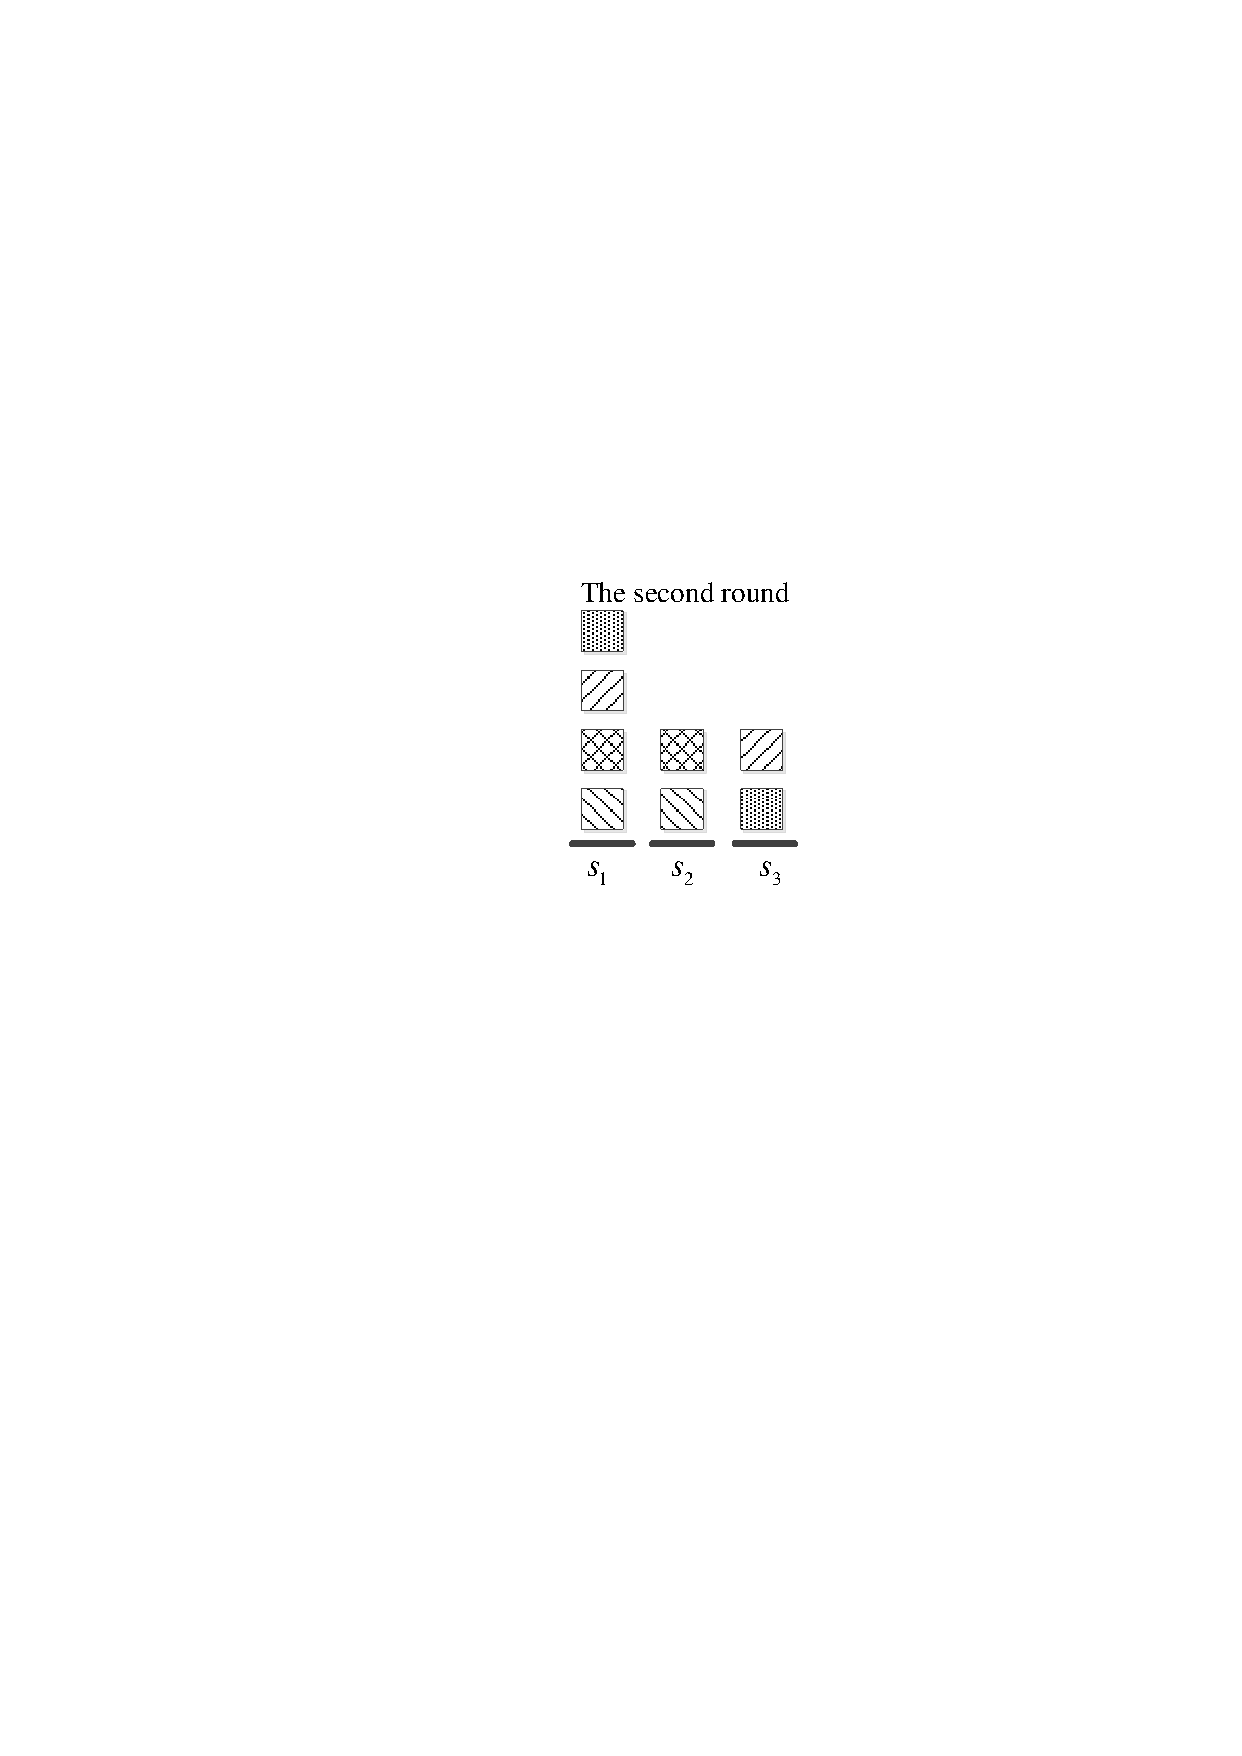
\includegraphics[width=0.155\columnwidth]{Figures/figure_combination_allocation_2}\label{figure_combination_allocation_2}}
%\renewcommand{\figurename}{abc}
\caption{The illustrative example for the allocation of tasks by combining overlapping tasks in each round.}
\label{figure_combination_allocation}
\end{figure}


For example, let $T\mathrm{=}\{t_1,t_2,t_3,t_4\}$ denote a task set where $t_1\mathrm{=<}0,3,3\mathrm{>}$, $t_2\mathrm{=<}2,6,2\mathrm{>}$, $t_3\mathrm{=<}3,8,4\mathrm{>}$ and $t_4\mathrm{=<}4,8,4\mathrm{>}$. There are three sensor nodes $s_1$, $s_2$, and $s_3$. Here $k\mathrm{=}3$ and $r\mathrm{=}2$. The task sets of these sensor nodes are marked as $T_1, T_2$, and $T_3$ with $T_1\mathrm{=}T_2\mathrm{=}T_3\mathrm{=}\{t_1,t_2,t_3,t_4\}$. We then maintain a quad list for each sensor node, i.e., $Q\mathrm{=}\{q_{12},q_{23},q_{24},q_{34}\}$ and sort $Q$  in the descending order based on the value of  data sharing. When Algorithm \ref{allocation_combine} is used to allocate tasks, the task pair $\mathrm{<}t_3,t_4\mathrm{>}$ is combined in the first round due to $d(t_3,t_4)\mathrm{=}4$. As illustrated in Fig. \ref{figure_combination_allocation_1}, tasks $t_3$ and $t_4$ should be allocated to sensor nodes. A new task $t_{34}\mathrm{=<}4,8,4\mathrm{>}$ is generated. We further remove tasks $t_3$ and $t_4$ from $T_1$, and add $t_{34}$ into $T_1$. After $t_3$ and $t_4$ are allocated, all the quads containing tasks $t_3$ and  $t_4$ will be removed from the quad list, i.e., $Q\mathrm{=}\{q_{12}\}$. Thus, tasks $t_1$ and $t_2$ should be combined and allocated to sensor nodes. As indicated in Fig. \ref{figure_combination_allocation_2}, after two rounds of task combination, tasks in $T$ are finally allocated to the sensor nodes in $S$, and the volume of sampled data has been computed.


%For example, let $T\mathrm{=}\{t_1,t_2,t_3,t_4\}$ denote a task set where $t_1\mathrm{=<}0,3,3\mathrm{>}$, $t_2\mathrm{=<}2,6,2\mathrm{>}$, $t_3\mathrm{=<}3,8,4\mathrm{>}$ and $t_4\mathrm{=<}4,8,4\mathrm{>}$. There are three sensor nodes $s_1$, $s_2$, and $s_3$. Here $k\mathrm{=}3$ and $r\mathrm{=}2$. The task sets of these sensor nodes are marked as $T_1, T_2$, and $T_3$ with $T_1\mathrm{=}T_2\mathrm{=}T_3\mathrm{=}\{t_1,t_2,t_3,t_4\}$. We then maintain a quad list for each sensor node, i.e., $Q\mathrm{=}\{q_{12},q_{23},q_{24},q_{34}\}$ and sort $Q$  in the descending of the overlap value. When the Algorithm \ref{allocation_combine} is used to allocate tasks, the task pair $\mathrm{<}t_3,t_4\mathrm{>}$ is combined in the first round due to t_3,t_4)\mathrm{=}4$. A new task $t$, i.e., $t\mathrm{=<}4,8,4\mathrm{>}$ is generated. We further remove tasks $t_3$ and $t_4$ from $T_1$, and add $t$ into $T_1$. After $t_3$ and $t_4$ are allocated, all the quads containing task $t_3$ and  $t_4$ will be removed from the quad list, i.e., $Q\mathrm{=}\{q_{12}\}$. In the next round, tasks $t_1$ and $t_2$ is executed to combine. The steps of combination are listed in Fig. \ref{figure_combination_allocation_1} where $`\surd$' means to allocate tasks due to the combination, and $`\times$' means to remove the sampling tasks which have been allocated to $r$ nodes. The details of the task allocation in presented in Fig. \ref{figure_combination_allocation_2}.
%
%\begin{figure}[t]
%\centering
%\subfigure[The procedures of combination by using Algorithm \ref{allocation_combine}.]{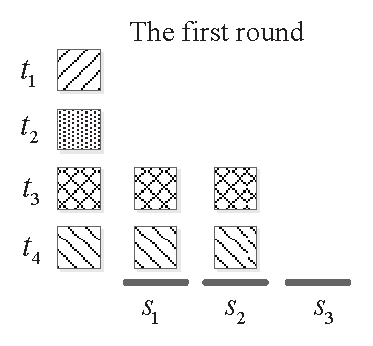
\includegraphics[width=0.9\columnwidth]{Figures/figure_combination_allocation_1}\label{figure_combination_allocation_1}}
%\subfigure[Two rounds of combination.]{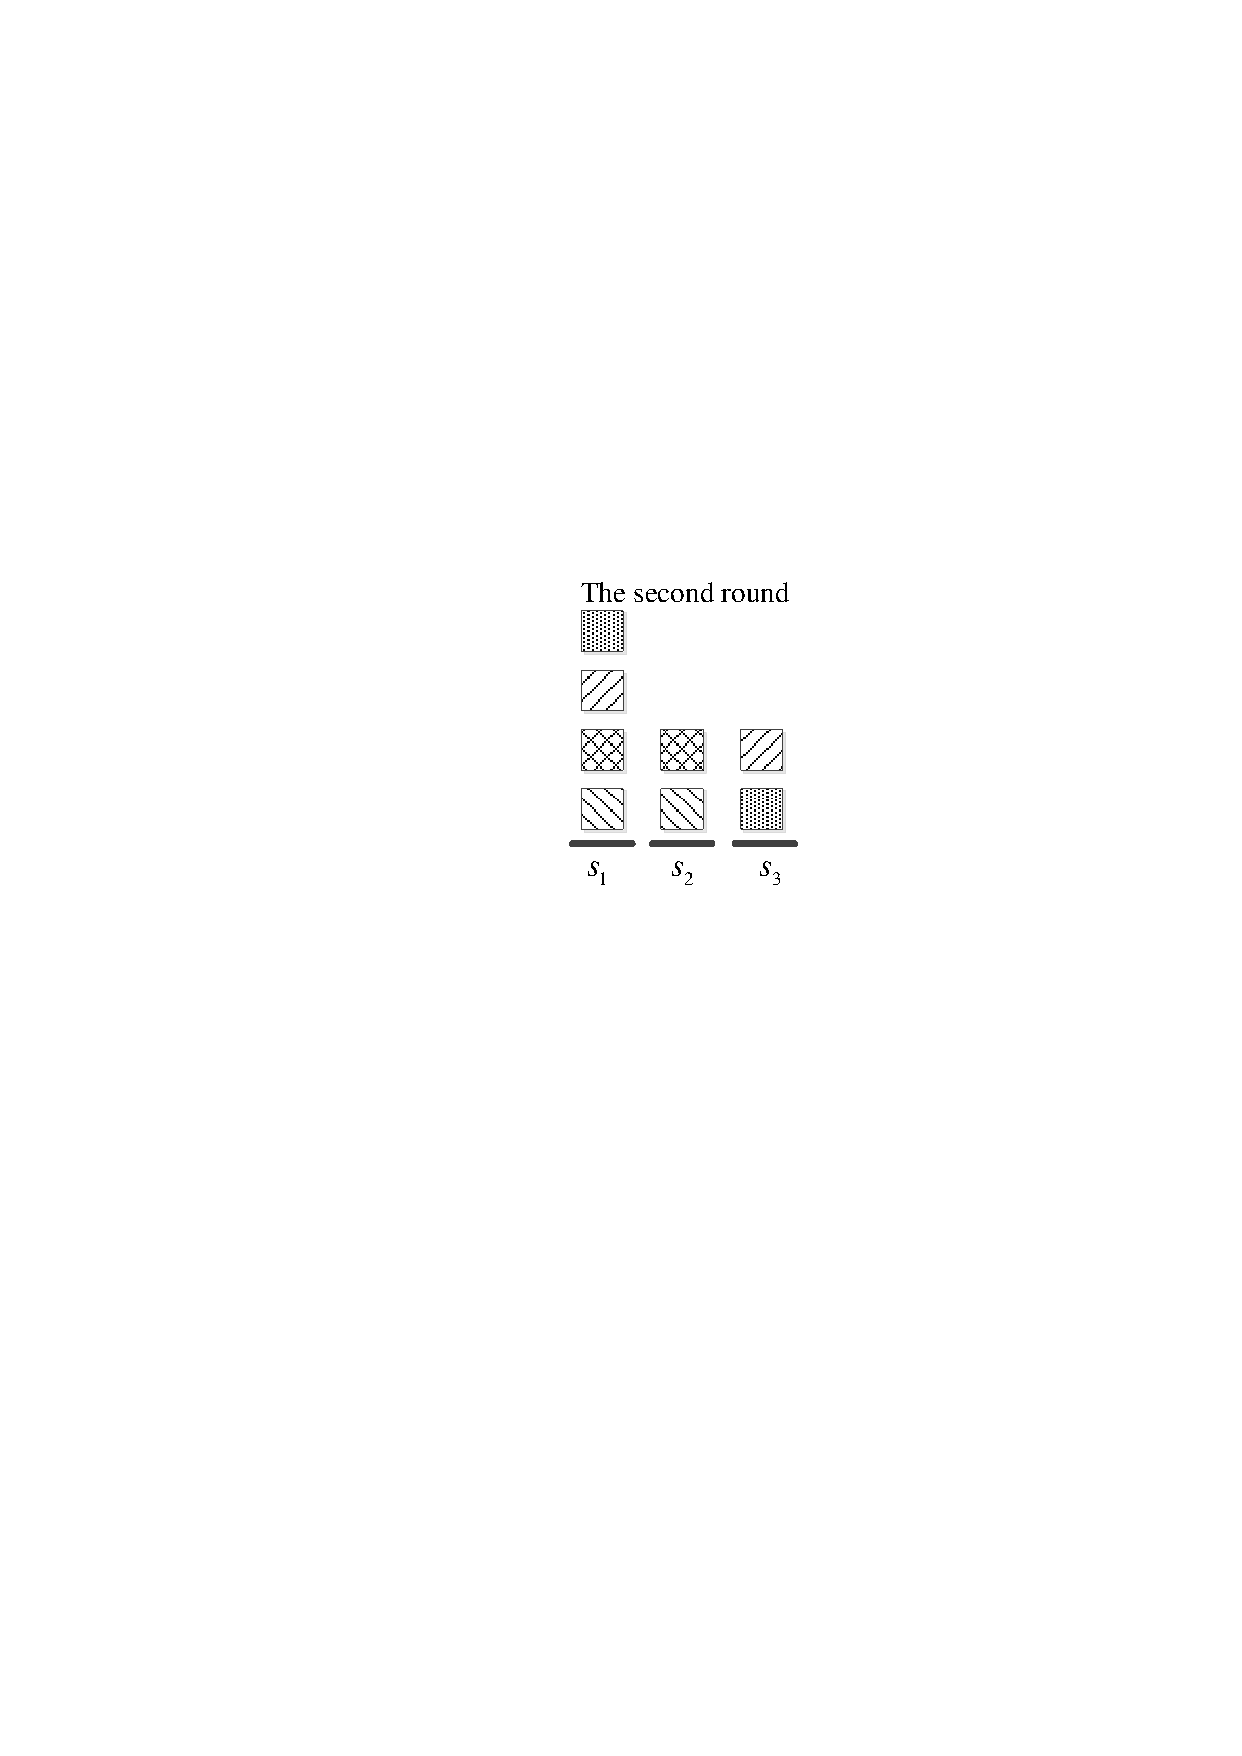
\includegraphics[width=0.8\columnwidth]{Figures/figure_combination_allocation_2}\label{figure_combination_allocation_2}}
%%\renewcommand{\figurename}{abc}
%\caption{Task allocation according to the combination operation. These tasks are identified by different colors.}
%\label{figure_combination_allocation}
%\end{figure}


In Algorithm \ref{allocation_combine}, lines $1\mathrm{-}2$ maintain a global quad list. Lines $3\mathrm{-}7$ present the combination of the overlapping tasks. Lines $8\mathrm{-}11$ ensure that all tasks are allocated even though some tasks are not overlapping with other sampling tasks. The time complexity is $O(n^2)$, and the space complexity is $O(n^2)$. If  Algorithm \ref{algorithm_combine2} is used to compute to sampled data for a task set, then the space and time complexity of Algorithm \ref{allocation_combine} are $O(1)$ and $O(n^2)$, respectively.

\begin{theorem}
Algorithm \ref{allocation_combine} is a 2-factor approximation allocation algorithm.
\label{theorem_allocation}
\end{theorem}

\begin{proof}
When $r\mathrm{=}k$,  the allocation solution is deterministic. We can allocate tasks to all of its candidate sensor nodes. Algorithm \ref{allocation_combine} means to run Algorithm \ref{algorithm_combine} on each sensor node for its allocated tasks. It always returns a 2-factor approximate result for each sensor node.  Algorithm \ref{allocation_combine} is thus a 2-factor approximation algorithm.

When $1\mathrm{\leq} r \mathrm{<} k$, Algorithm \ref{allocation_combine} selects a task pair with the maximal value of data sharing from the task set repeatedly. Algorithm \ref{allocation_combine} can be transformed to  Algorithm \ref{algorithm_combine}. The process of transformation can be described as follows:
\begin{itemize}
\item Compute the value of data sharing between overlapping tasks which may be allocated to a same node.
\item For any two tasks which are not allocated to a same node, we set its the value of data sharing to negative infinity.
\item If overlapping tasks  have been allocated to a node, the data sharing between them will be adjusted to negative infinity.
\item If a task has been allocated to $r$ nodes, data sharing between it and other nodes will be set to negative infinity.
\end{itemize}

Then perform Algorithm \ref{algorithm_combine} on the task set until there is no overlapping tasks.  We get the minimal volume of sampled data. Meanwhile, we get a sampling interval set $\Phi$ in which none of intervals are overlapping. An interval $I$ in $\Phi$ satisfies several sampling tasks. Thus, we get several sets of tasks. Since a task has been allocated to $r$ nodes, these sets of tasks are the result of task allocation. Therefore, the computation of the volume of sampled data can be solved by running the Algorithm \ref{algorithm_combine} repeatedly. The performance of Algorithm \ref{algorithm_combine} has been proved by Theorem \ref{theorem_schedule} and returns a 2-factor approximate result of the volume of sampled data. Thus, Algorithm \ref{allocation_combine} is a 2-factor approximation algorithm.
%
%When $r\mathrm{=}k$,  the allocation solution is deterministic. We can allocate tasks to all of its candidate sensor nodes. Algorithm \ref{allocation_combine} means to run Algorithm \ref{algorithm_combine} on each sensor node for its allocated task set. It always returns a 2-factor approximation result for each sensor node.  Algorithm \ref{allocation_combine} is thus a 2-factor approximation algorithm.
%
%When $1\mathrm{\leq} r \mathrm{<} k$, Algorithm \ref{allocation_combine} selects a task pair with the maximal overlap value from the task set repeatedly. In fact, an allocation problem can be constructed to a special case of a scheduling problem which maintains its performance. As shown in Fig. \ref{figure_proof_allocation}, assume there are five tasks $t_1,...,t_5$ (as indicated by cycle) and three node $s_1,s_2,s_3$. If $t_1,t_2,t_3$ can be allocated to $s_1$, $t_2,t_3,t_4$ can be allocated to $s_2$ and $t_3,t_4,t_5$ can be allocated to $s_3$. Here, $k\mathrm{=}3$ and $r\mathrm{=}2$. The procession of construction can be described as follows:
%\begin{itemize}
%\item Compute the overlap between overlapping tasks which may be allocated to a same node (as indicated by real lines in Fig. \ref{figure_proof_allocation}).
%\item For any two tasks which are not allocated to a same node, we set its overlap value to negative infinity (as indicated by dotted lines in Fig. \ref{figure_proof_allocation}).
%\item If  tasks $t_i$ and $t_k$ have been allocated to a node $s_j$, the overlap between them will be adjusted to negative infinity.
%\end{itemize}
%Then the allocation problem, MIN-SAA, can be solved by running the Algorithm \ref{algorithm_combine}. The performance of Algorithm \ref{algorithm_combine} has been proved by Theorem \ref{theorem_schedule} and achieves a 2-factor approximation result of data sampling. Thus, Algorithm \ref{allocation_combine} is a 2-factor approximation algorithm.
\end{proof}

\begin{figure}[t]
\centering
\subfigure{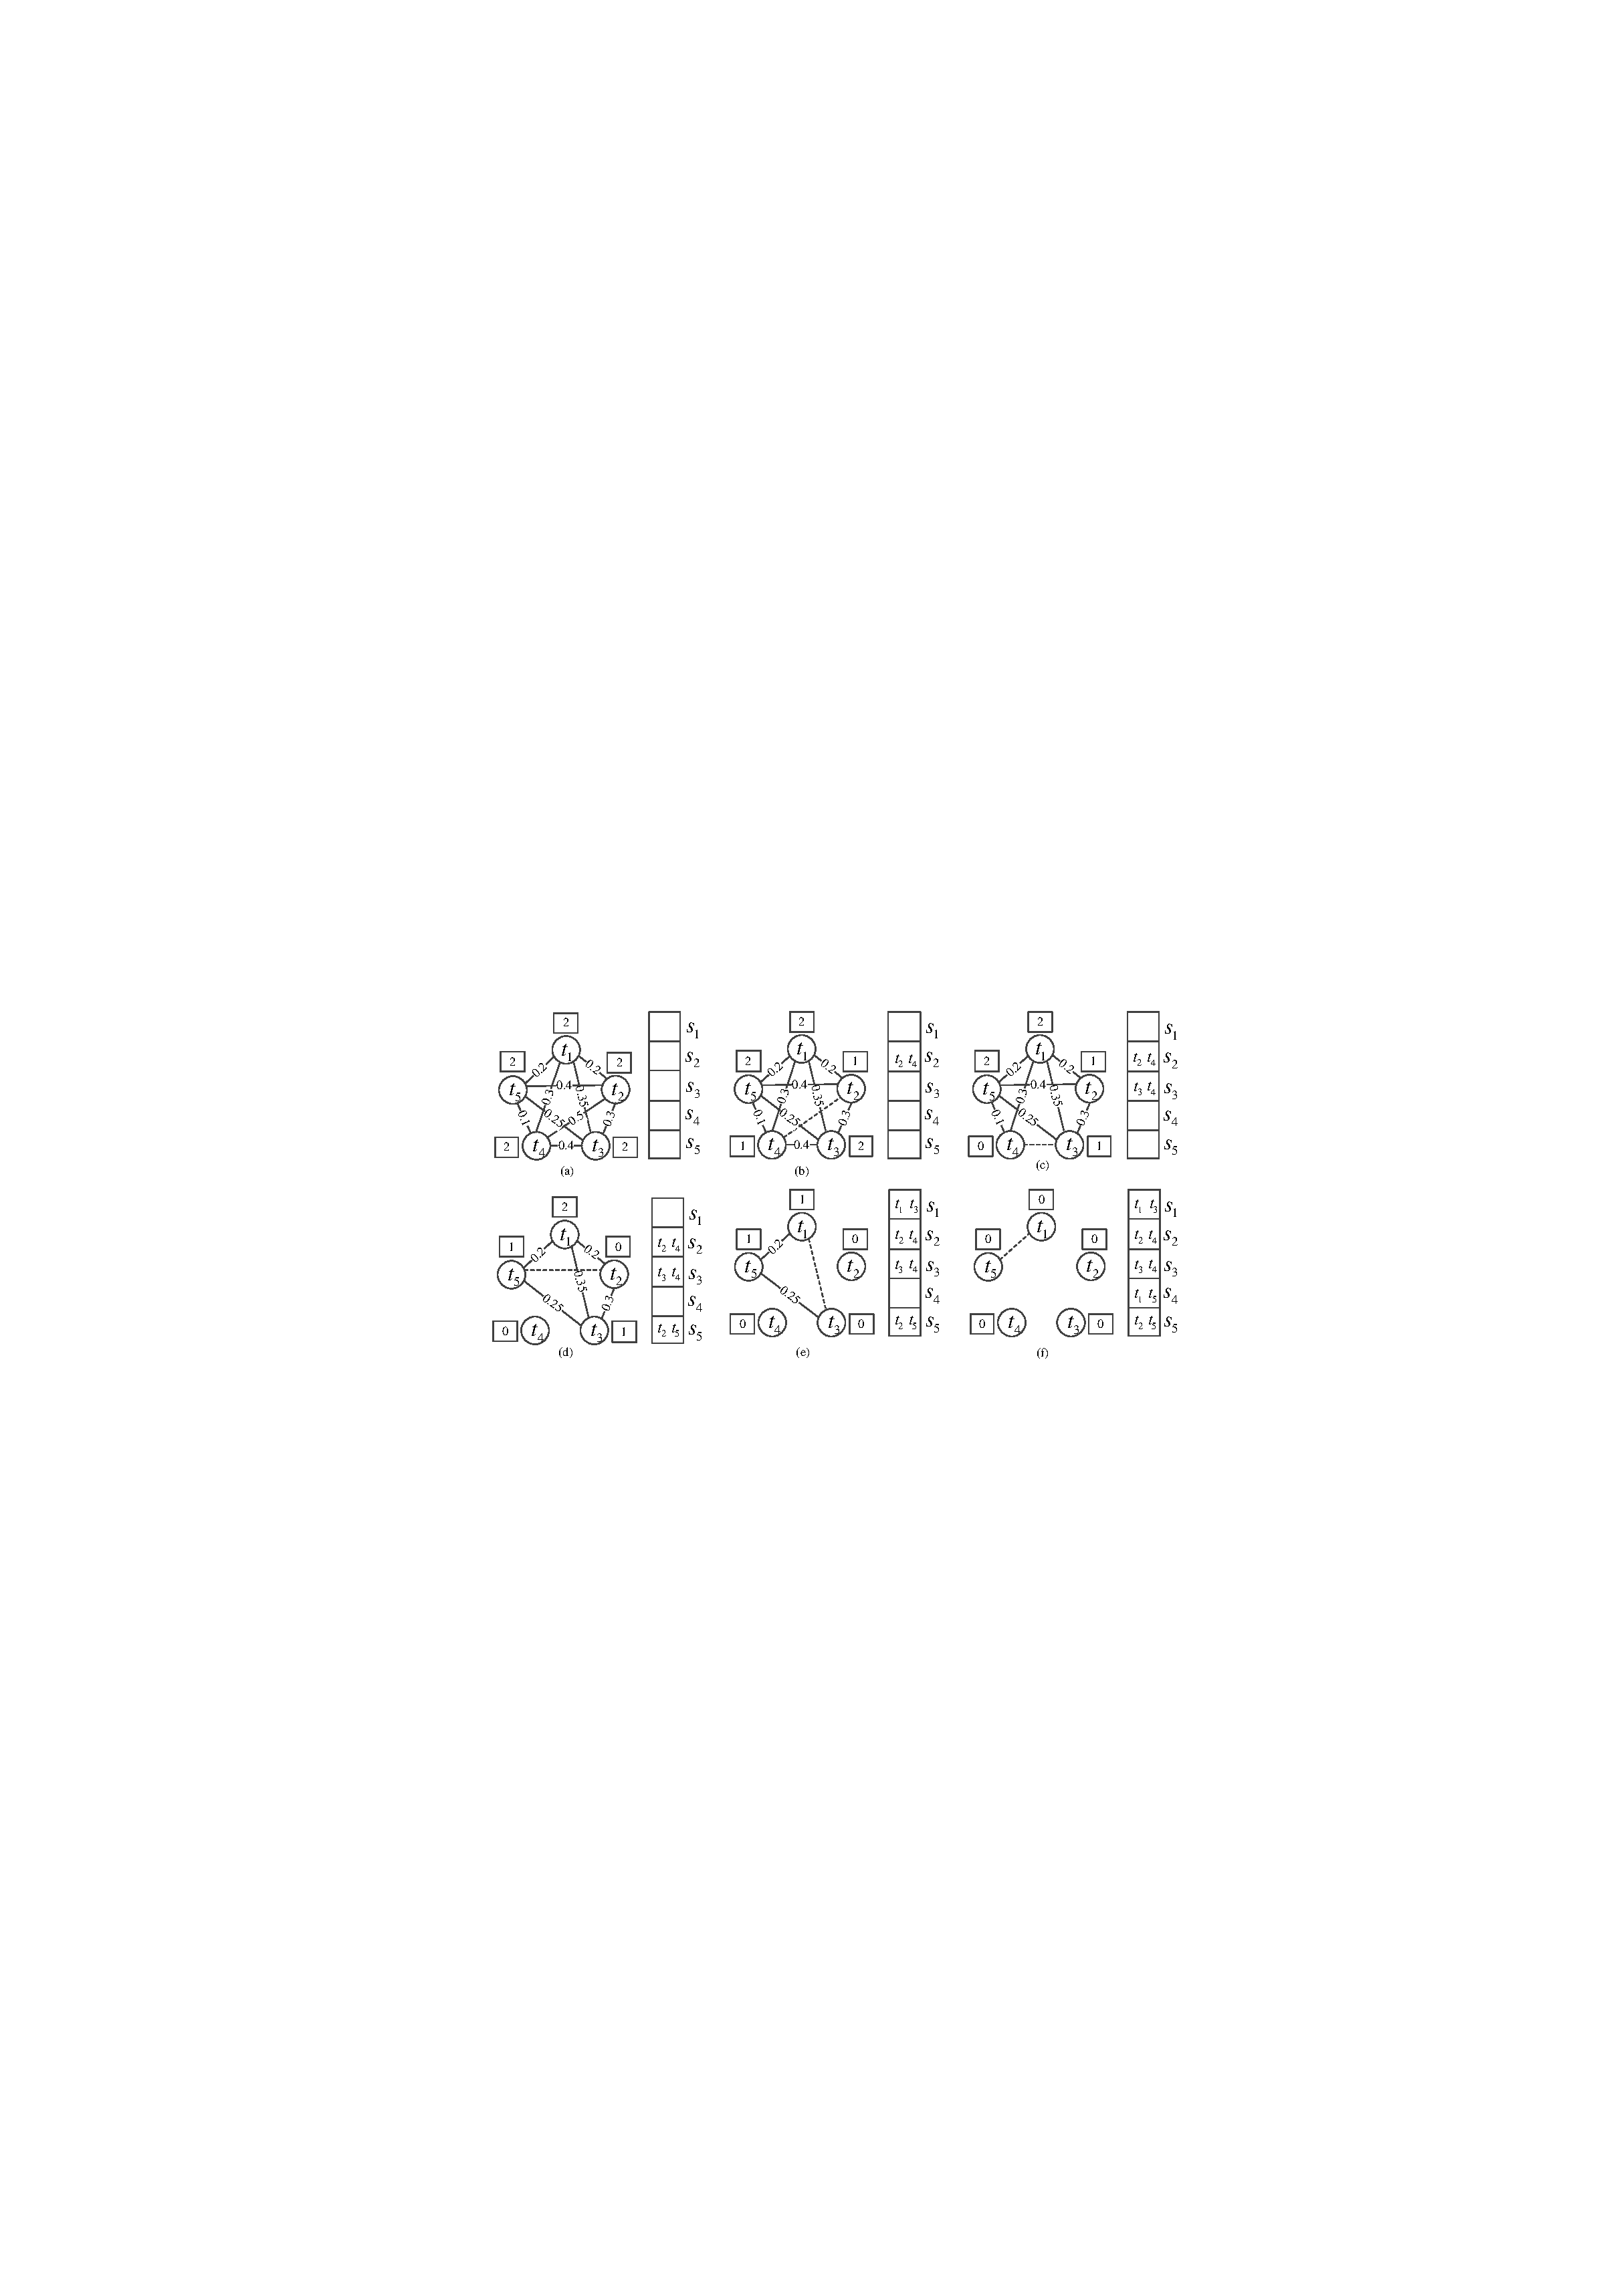
\includegraphics[width=0.85\columnwidth]{Figures/figure_proof_allocation}}
\caption{The illustrative example of transformation from Algorithm \ref{allocation_combine} to Algorithm \ref{algorithm_combine} by combining the overlapping tasks which have the maximal value of data sharing in each step. Here, $k\mathrm{=}3$ and $r\mathrm{=}2$.}
\label{figure_proof_allocation}
\end{figure}

To be clear, we take an example to illustrate the process of transformation. As shown in Fig. \ref{figure_proof_allocation}, assume there are five tasks $t_1,...,t_5$ (as indicated by cycles) which should be allocated to five nodes $s_1,...,s_5$.  \{$t_1,t_2,t_3$\} are detected by $s_1$. Similarly,  \{$t_2,t_3,t_4$\}, \{$t_3,t_4,t_5$\}, \{$t_4,t_5,t_1$\} and \{$t_5,t_1,t_2$\} are detected by nodes $s_2$, $s_3$, $s_4$ and $s_5$, respectively. Here, $k\mathrm{=}3$ and $r\mathrm{=}2$. As illustrated in Fig. \ref{figure_proof_allocation}(a), we construct a weighted graph where a vertex stands for a task. If two tasks are overlapping, then a weighted edge exists. The weighted value represents the value of data sharing. The value in the rectangle indicates the number of nodes which the task has been allocated to. The overlapping tasks which have the maximal data sharing are allocated to a node. Then, the data sharing between them is set to negative infinity (indicated by the dotted line). If a task has been allocated to $r$ sensor nodes, then the task is removed from the task set. Without loss of generality, the new tasks generated from the combination of original tasks are not demonstrated. For example, in Fig. \ref{figure_proof_allocation}(b), we find that tasks $t_2$ and $t_4$ have the maximal value of data sharing: $0.5$. Then, allocate them to the node $s_2$, and set the data sharing between them to be negative infinity. As illustrated in Fig. \ref{figure_proof_allocation}(d), when the task $t_4$ has been allocated to $s_2$ and $s_3$, the edges between it and other nodes are removed. When the sampling interval of tasks are scheduled to achieve the maximal data sharing, these tasks are eventually allocated to and sampled by the nodes. Since the process of task combination will generate new tasks, new vertices will added to the graph, but this will not impact the performance of Algorithm \ref{allocation_combine}.

%\begin{figure}[t]
%\centering
%\subfigure{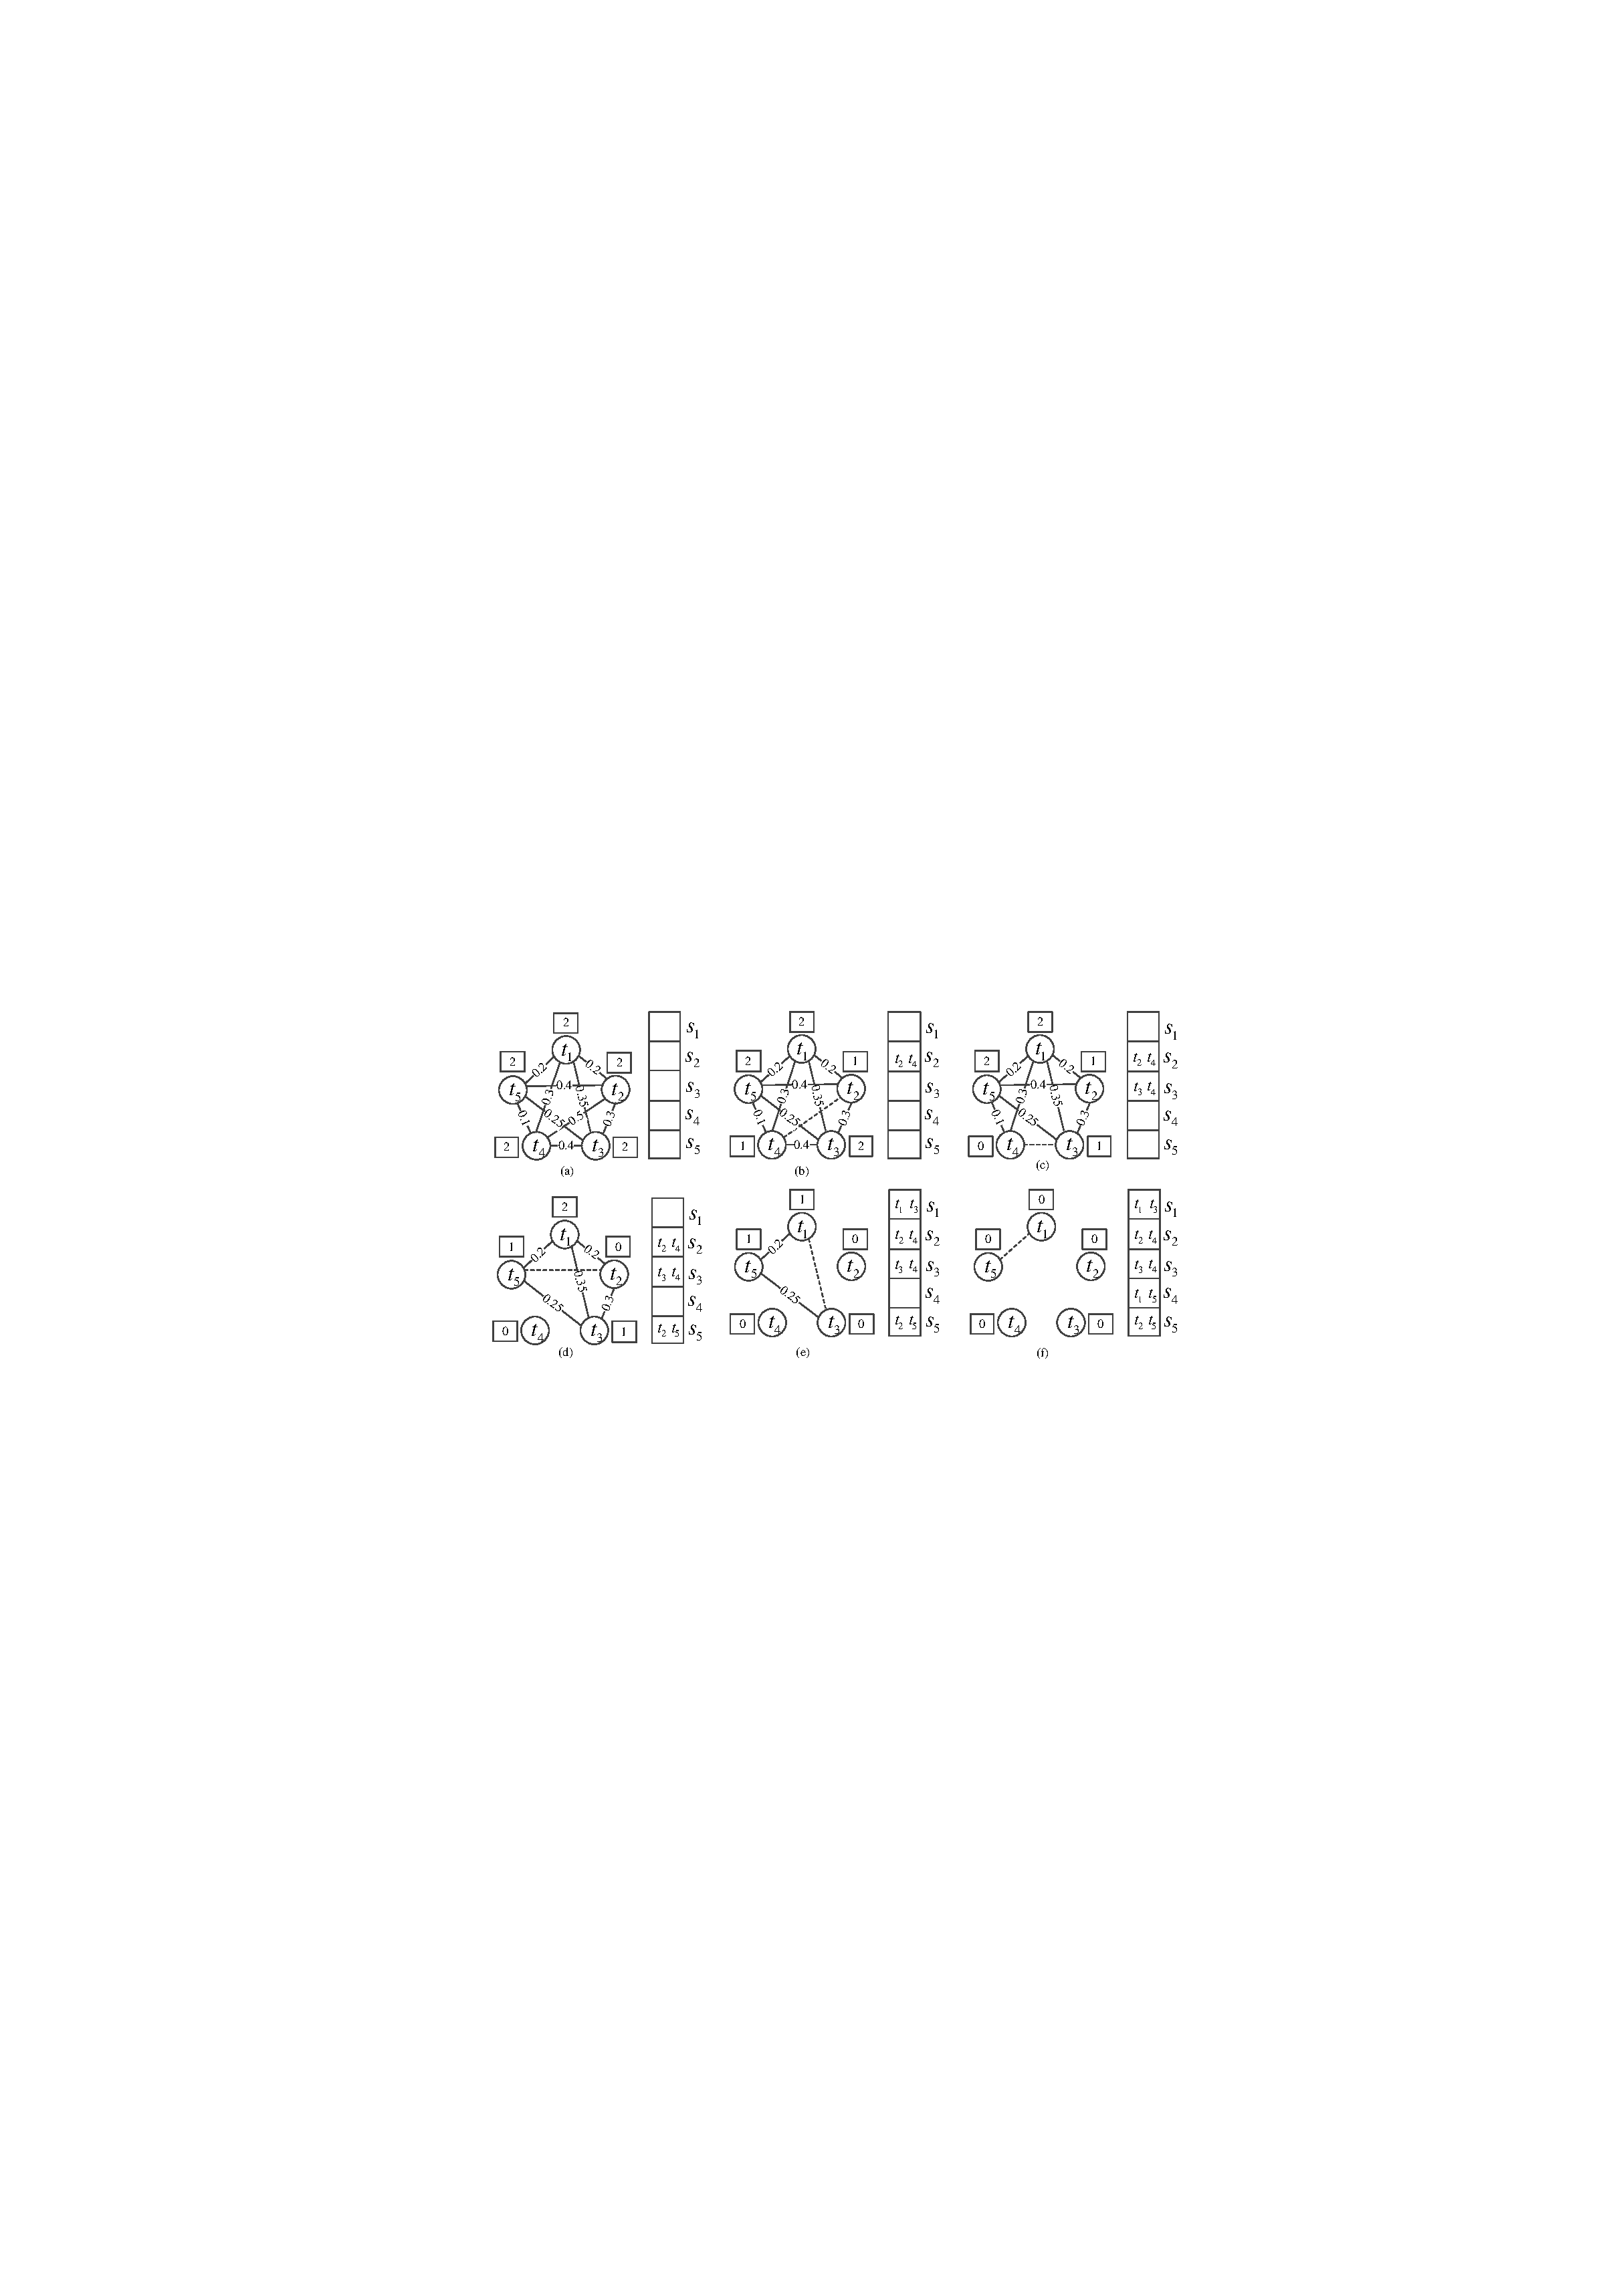
\includegraphics[width=0.6\columnwidth]{Figures/figure_proof_allocation}}
%%\renewcommand{\figurename}{abc}
%\caption{The allocation problem, MIN-SAA, can be transformed to a special case of scheduling problem, MIN-SA.}
%\label{figure_proof_allocation}
%\end{figure}


%\subsection{Discussion}
%The allocation of tasks involves assigning each task to $r$ out of $k$ candidate sensor nodes. The current allocation scheme seeks to fully exploit the benefits of data sharing amongst tasks on sensor nodes. In reality, there still exist other important constraints that can be exploited to improve the proposed allocation schemes. Note that each sensor node is resource-constrained, i.e., it has limited computation and memory resources. If a sensor node has been allocated many sampling tasks, it may not handle all the tasks timely and exhaust the energy at early time. This problem cannot be simply addressed by limiting the number of tasks a sensor node carrying. The reason is that even the number of tasks allocated to the sensor nodes is same, but the real work load of  sensor nodes may have a considerable difference due to the data sharing strategy. Therefore, contemporary task allocation schemes can be more practical if we consider the load balance amongst sensor nodes. An effective method is to set a threshold for the constrained resource. Each allocation step makes sure that the threshold value is not exceeded. Algorithm \ref{allocation_prune} and Algorithm \ref{allocation_combine} are flexible to adjust for this tactics. When the  limited resource changes dynamically, the allocation problem will be more difficult to solve. We leave it as our future work.
%
%In this paper, we aim to minimize the sampled data for a sampling task set by cooperatively scheduling and allocating tasks. Our proposed algorithms focus on the procedures of task allocation and scheduling and do not relay on the topology of a network. In fact, the information of a network such as the routing protocol can be utilized to improve the performance of our algorithms on many respects. For example, even though many applications require to get the entire data of a sampling interval, we can depart the sampling interval into several segments for a $k$-coverage network if these segments can be integrated into the complete task finally. These sampling segments can be allocated to the sensor nodes, which will help to balance the sampling workload on sensor nodes in our proposals. However, embedding the network information into our solutions introduces arduous problems, including task dividing, data fusion and so forth. We leave it as our future work as well.

\section{Performance evaluation}
\label{section_evaluation}
In this section, we first introduce our experimental environment and settings. Then, we evaluate the effectiveness of our proposed algorithms by using a physical testbed containing $50$ wireless sensor nodes. Finally, a widely-used simulation tool, i.e., TOSSIM, is used to verify the scalability of our proposals.

\subsection{Experimental environment and settings}
\begin{figure}[t]
\centering
\subfigure{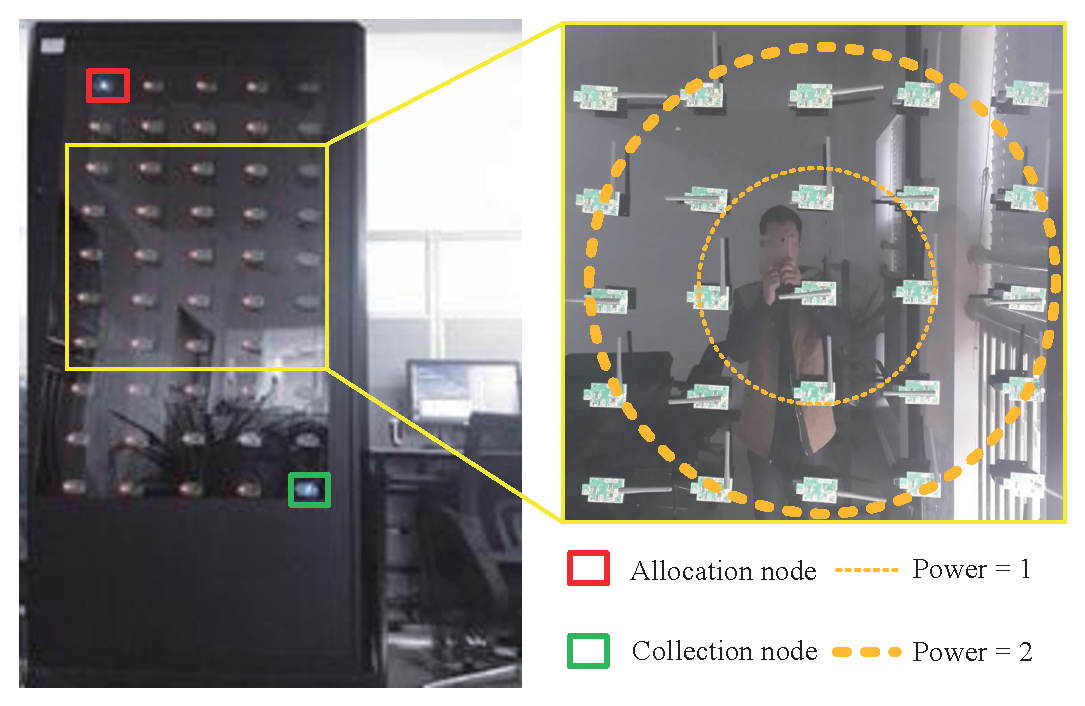
\includegraphics[width=0.55\columnwidth]{Figures/testbed_image}\label{figure_testbed_image}}
%\renewcommand{\figurename}{abc}
\caption{The transmission power can be adjusted to realize the $k$-coverage network  in the testbed.}
\label{figure_testbed}
\end{figure}



We evaluate the effectiveness of our proposed algorithms on a physical testbed of WSNs. As indicated in Fig. \ref{figure_testbed}, this testbed contains $50$ wireless sensor nodes. The distance between two adjacent sensor nodes is about $20$cm. In the experiments, we construct different $k$-coverage networks by adjusting transmission power of nodes. The parameter $k$ becomes large when the transmission power of nodes is increased. By default, the power is set to the lowest level, and the transmission range is only about tens of centimeters. All the nodes operate on the same channel.

With such settings, although a number of nodes locate in the same collision domain, the packet loss rate observed in the experiments is less than $0.1\%$. The reason is that the nodes in the same collision domain access the wireless channel for transmission based on the MAC protocol, and packet loss caused by severe interference will not happen \cite{2006_MAC_survey}, \cite{1994MACAW}.

Since the WSN is densely deployed, any two nodes can set up a wireless link by at most three hops. The proposed algorithms are implemented in a centralized manner which is widely used in actual systems \cite{2009greenorbs}, \cite{2009_oceansense}, \cite{2007_outlier_detection_mobihoc},\cite{2011_compressed_data_aggregation}. We use the left-top node (as highlighted by a red rectangular) as the sink node which allocates a task set to other nodes, and the right-bottom node as the collection node (as indicated by the green rectangular) which collects all sampled data. Transmitted packets are counted to indicate the required sampled data, while received packets are collected to demonstrate the actual collected data.

The value of $k$ is varied from $2$ to $8$, which is reasonable and always used in the practical WSN systems \cite{2013_TPDS_coverage}, \cite{2005_coverage_problem}. We construct a unit of continuous data by sampling temperature $5$ times per second, and sent the data by using a packet. The interval length of a sampling task is randomly generated and not greater than $10$. To be specific, the begin time of a sampling task is evenly distributed in time slot $[0,\;50]$. We  run each algorithm by $10$ times and use the average value of these results as the final result. To be clear, $m$, $n$, and $l$ represent the cardinality of the sensor node set and the task set, and the length of a sampling interval, respectively.


\subsection{Performance of data sharing for a sampling task set}

At first, we evaluate the performance of our Algorithm \ref{algorithm_combine}, denoted by `\textit{Overlap}', which returns a reorganized sampling task set based on the idea of data sharing, against the state-of-the-art method \cite{2013fang}, named `\textit{GA}' here. \emph{GA} is an approximation algorithm for optimizing the data sampling of a task set on a single sensor node. Meanwhile, \emph{GA} can derive the optimal scheduling algorithm, named as `\textit{DP}', using dynamic programming technique on the condition that all tasks have the same interval length. In this experiment, the interval length of each sampling task is consistently set to $5$, and the window size of each task varies from $5$ to $15$.

%A sampling task is randomly generated in the time slot $[0,\; 50]$.
\begin{figure*}[t]
\centering \subfigure[$l\mathrm{=}5$]{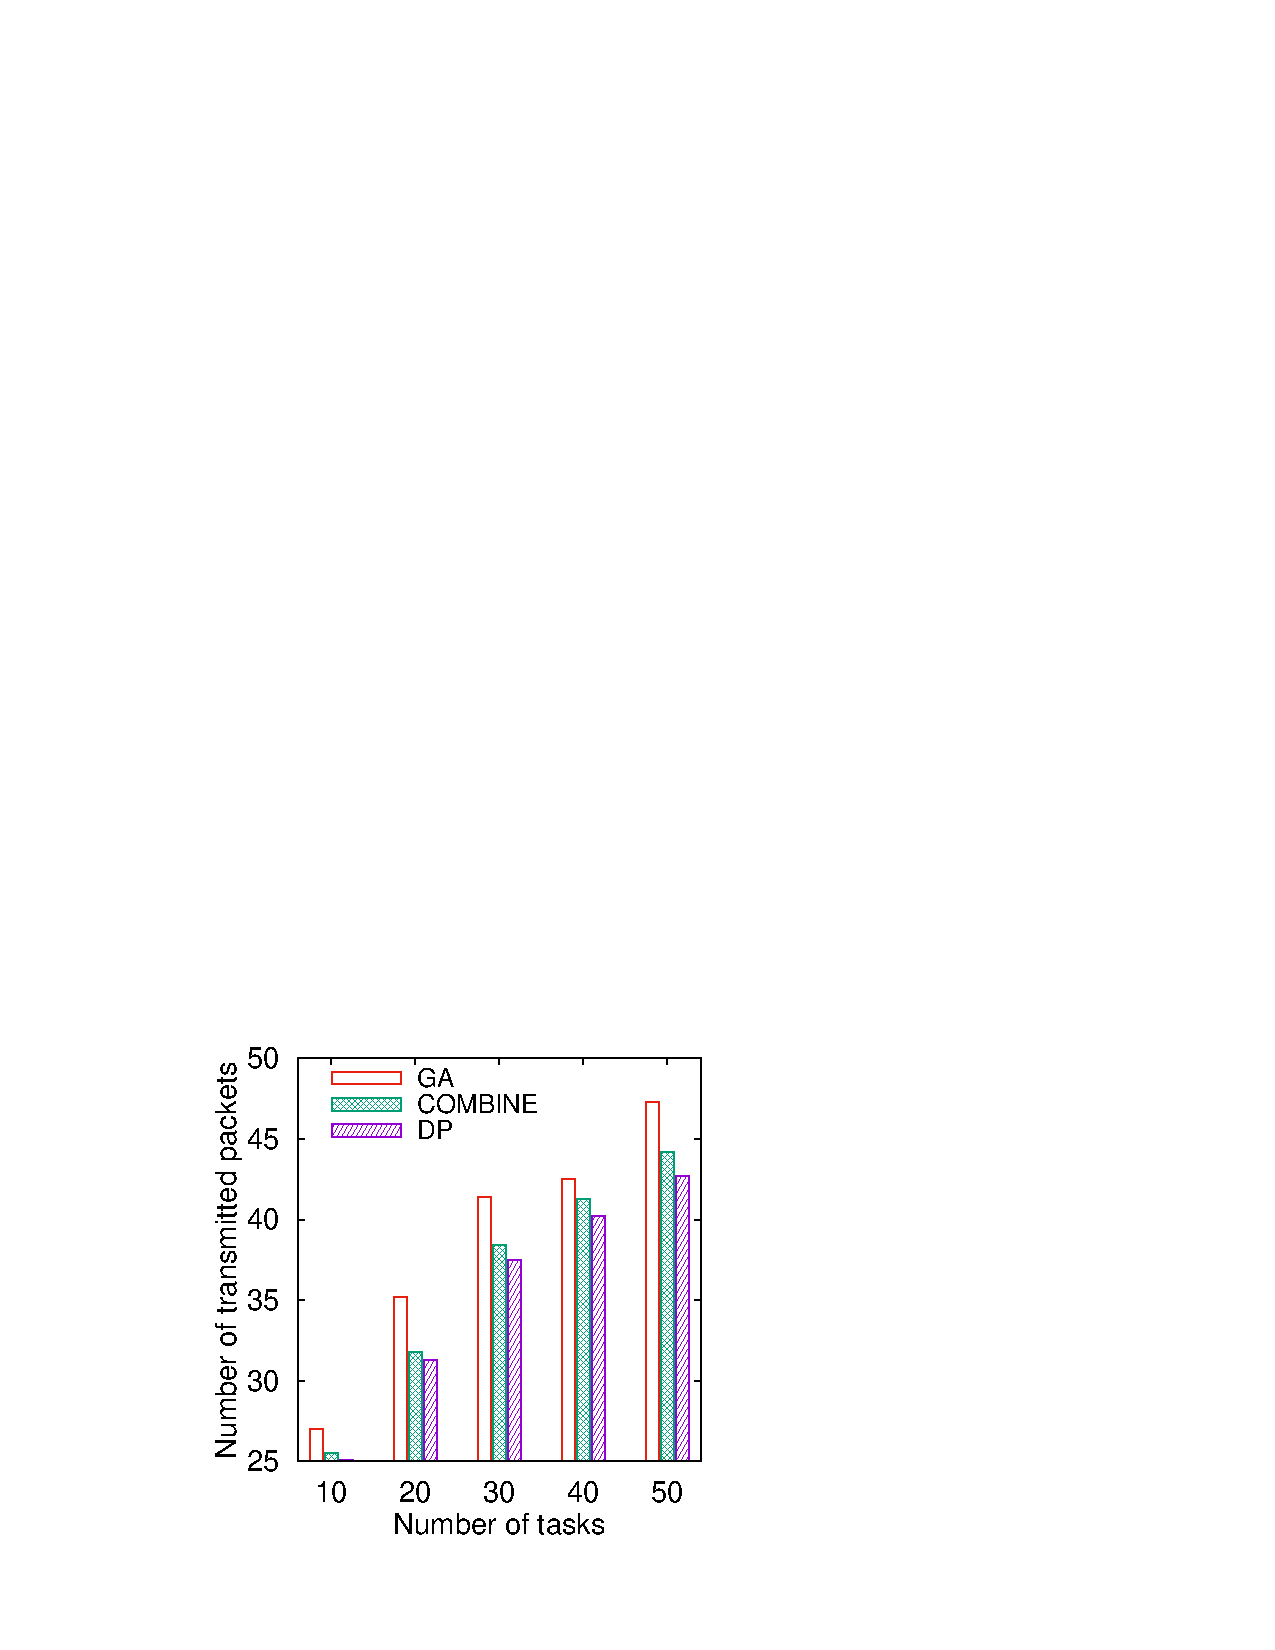
\includegraphics[width=0.233\columnwidth]{Figures/evaluation1_data_sampled_tasks}\label{evaluation1_data_sampled_tasks}}
 \subfigure[$n\mathrm{=p}30$]{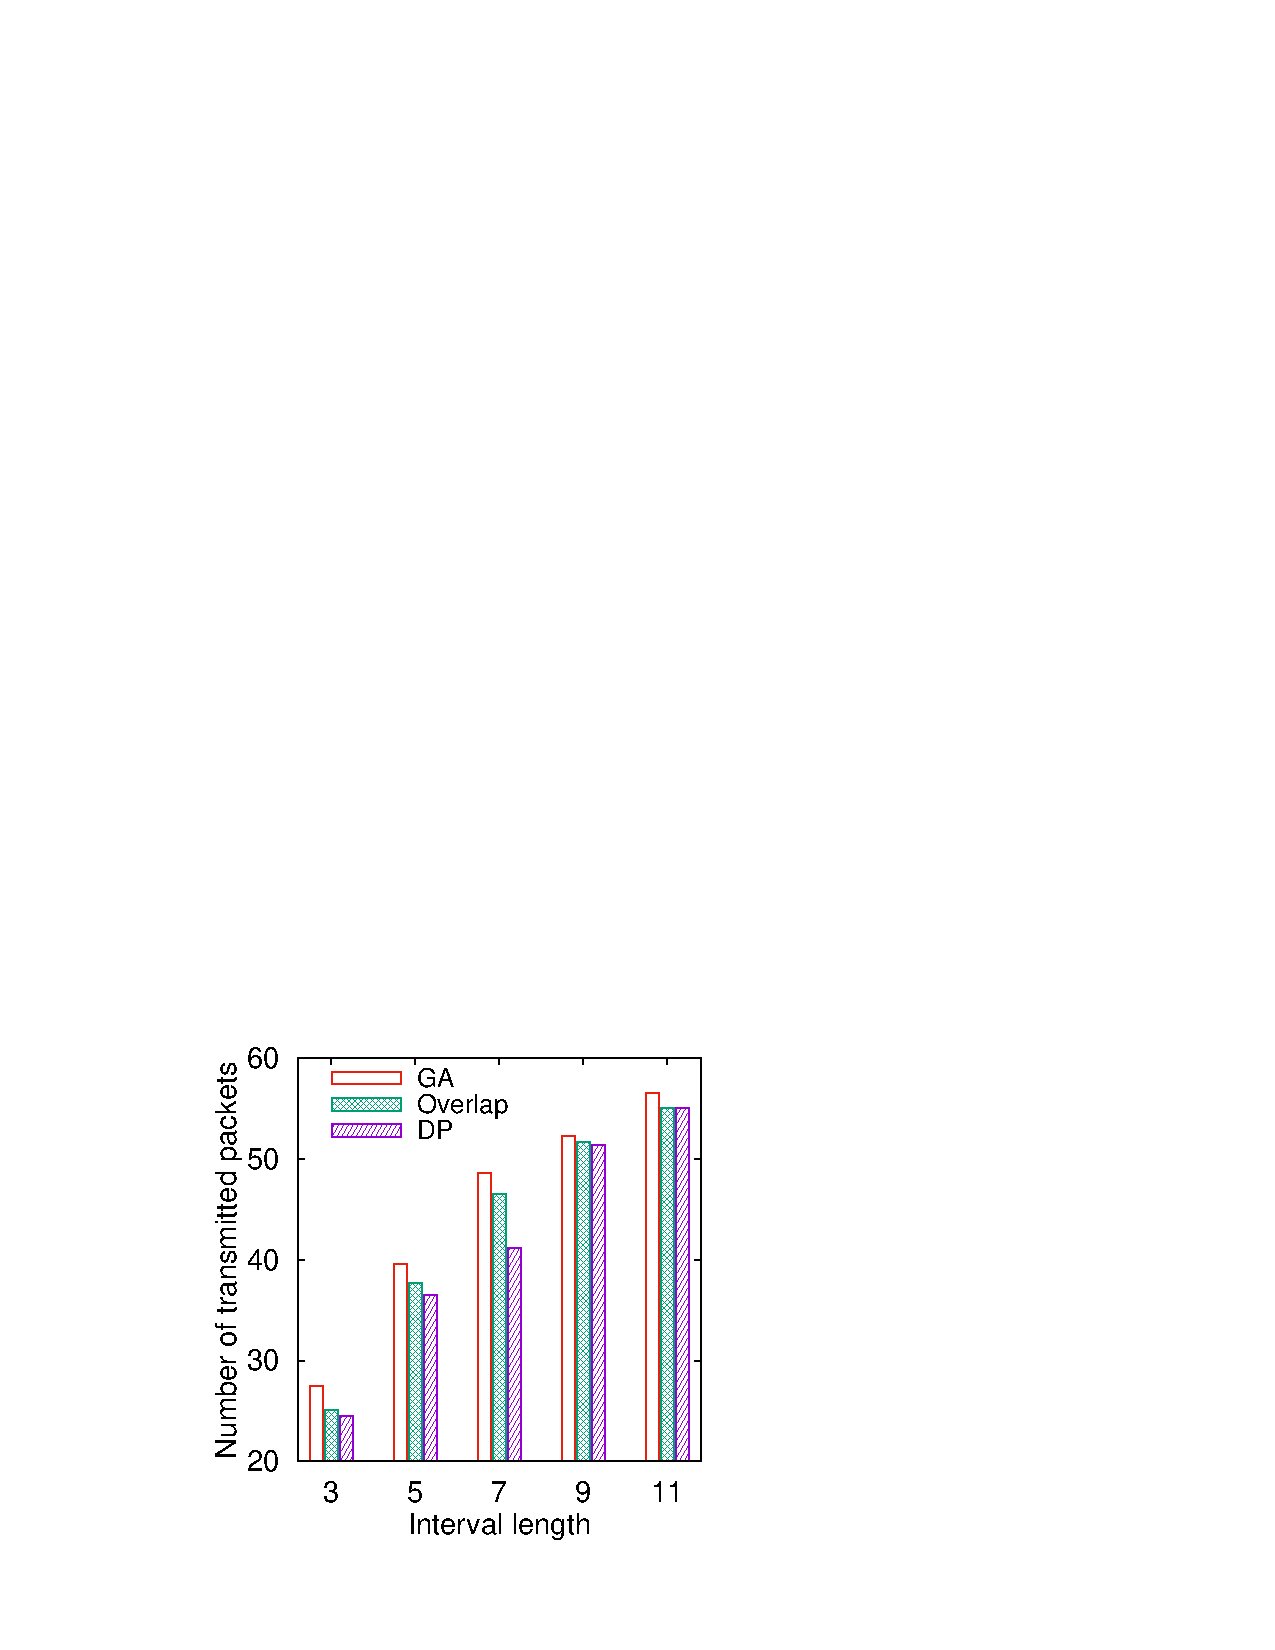
\includegraphics[width=0.233\columnwidth]{Figures/evaluation1_data_sampled_interval}\label{evaluation1_data_sampled_interval}}
\subfigure[$l=5$, $n=30$ ]{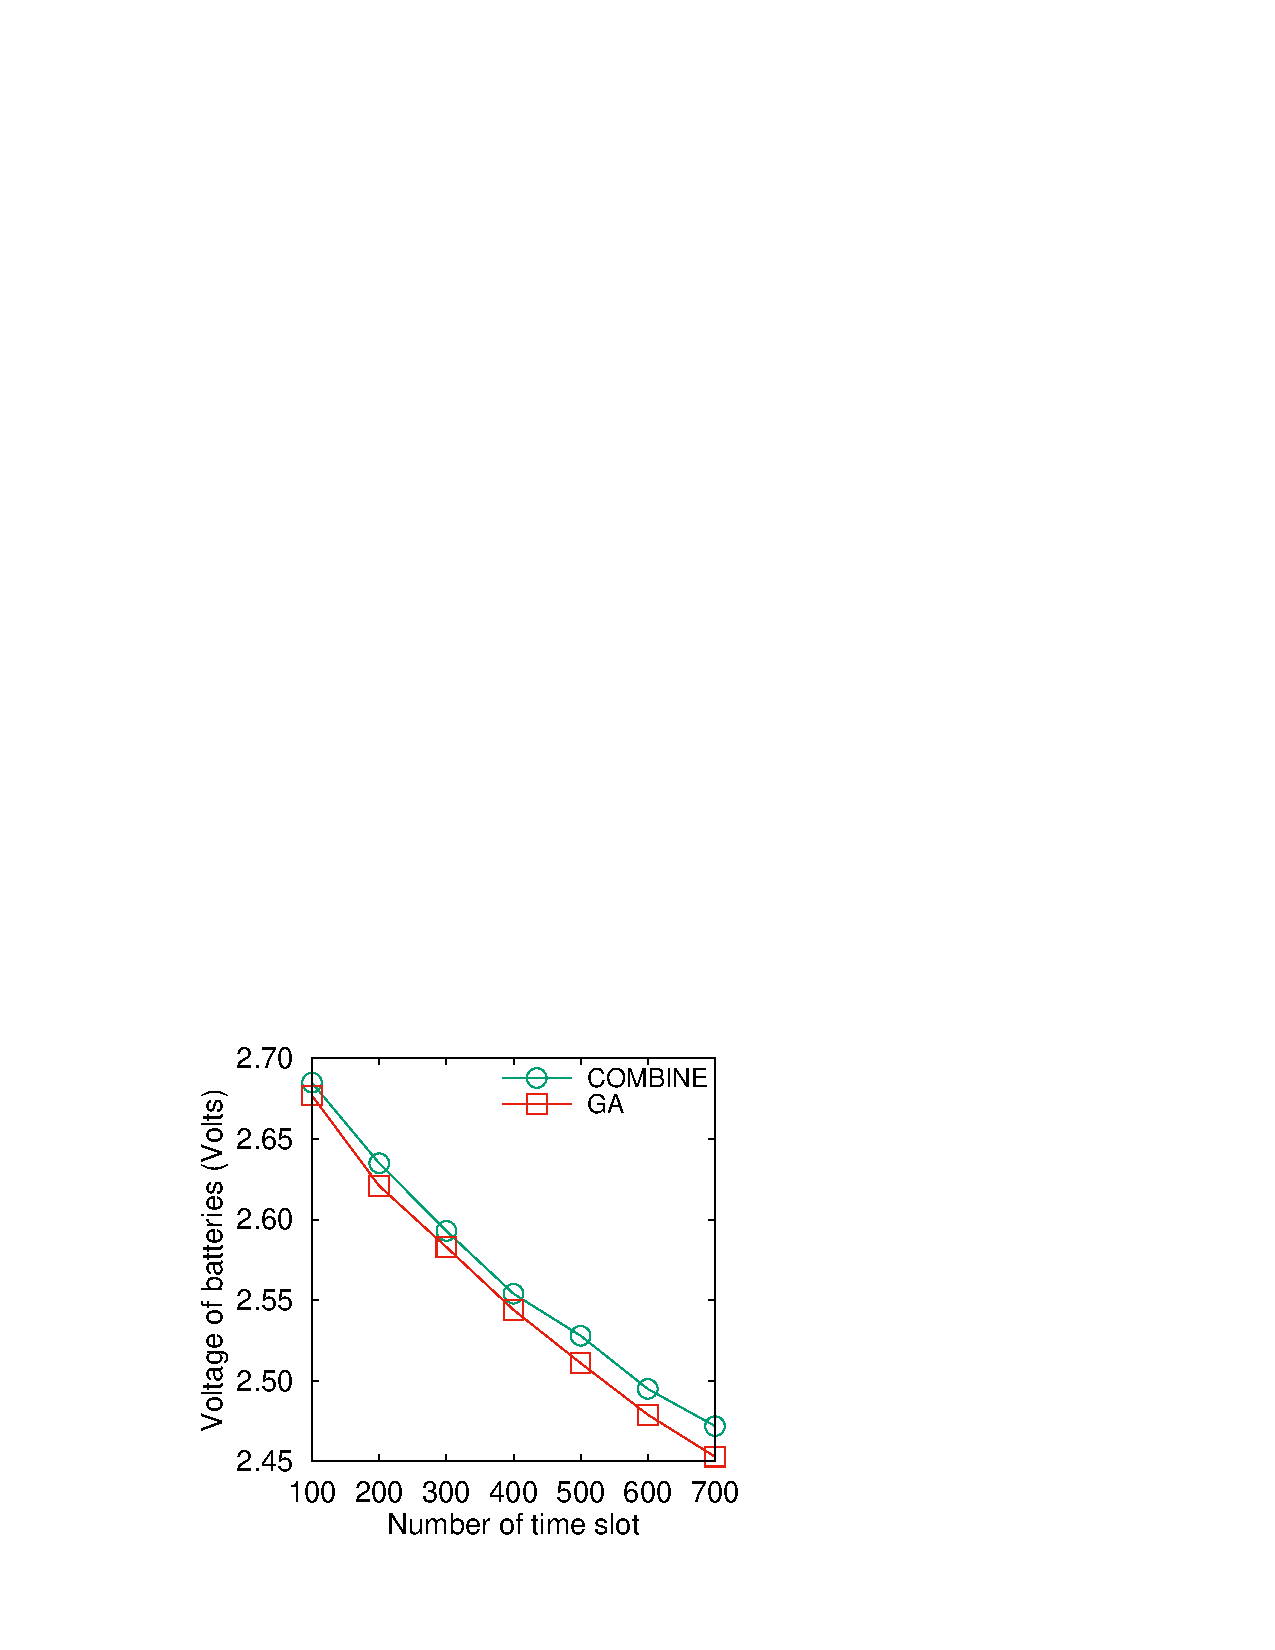
\includegraphics[width=0.258\columnwidth]{Figures/evaluation1_voltage}\label{evaluation1_voltage}} \subfigure[$l\mathrm{=}5$]{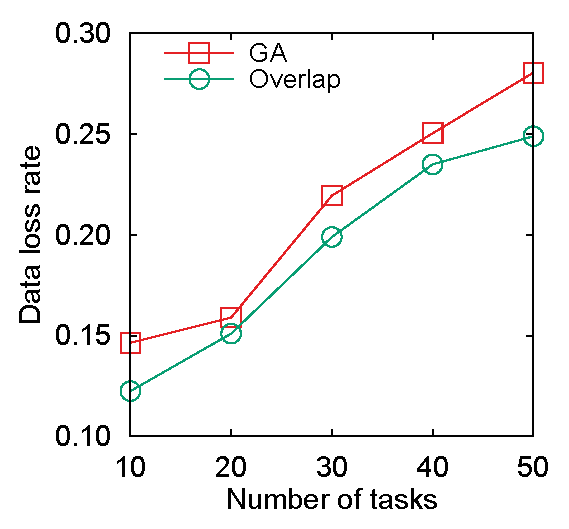
\includegraphics[width=0.252\columnwidth]{Figures/evaluation1_data_loss_rate}\label{evaluation1_data_loss}}
%\renewcommand{\figurename}{abc}
\caption{A comparison of the number of transmitted packets by varying the number of tasks in (a), and the interval length in (b). Energy consumption is compared by varying the number of time slot in (c), and data loss rate in (d).}
\label{evaluation1_data_sampled}
\end{figure*}


%Fig. 6(a)-(b)
Fig. \ref{evaluation1_data_sampled_tasks} and Fig. \ref{evaluation1_data_sampled_interval} illustrate the number of transmitted packets of task scheduling methods, i.e., \emph{Overlap}, \emph{GA} and \emph{DP}, by varying the cardinality of a sampling task set (Fig. \ref{evaluation1_data_sampled_tasks}) or  the interval length of a sampling task (Fig. \ref{evaluation1_data_sampled_interval}). Specifically, the interval length of a sampling task is set to $5$ in Fig. \ref{evaluation1_data_sampled_tasks} while the cardinality of each task set is fixed to $30$ in Fig. \ref{evaluation1_data_sampled_interval}. It is easy to observe from Fig. \ref{evaluation1_data_sampled_tasks}  and Fig \ref{evaluation1_data_sampled_interval} that the number of transmitted packets increases with the  growth of both the number of tasks and the interval length. However, our \emph{Overlap} method performs better and returns smaller number of transmitted packets  than \emph{GA}. This happens because our scheduling algorithm combines the maximal overlapping tasks each time. Thus, every scheduling step is the current optimal choice. Considering \emph{GA} schedules tasks based on the end time of a task, it cannot make sure each scheduling choice is optimal. That is the reason why the \emph{Overlap} outperforms the \emph{GA}. Meanwhile, Fig. \ref{evaluation1_data_sampled_tasks} and Fig. \ref{evaluation1_data_sampled_interval} indicate \emph{Overlap} achieves 2-factor approximation result vs. the optimal result. This verifies the correctness of  the Theorem \ref{theorem_schedule}.

In Fig. \ref{evaluation1_voltage}, we run  both \emph{Overlap} and \emph{GA} methods on two sensor nodes to test their energy usage. The terminal voltage of batteries equipped for a sensor node is measured every $100$  time slots. The initiate value is $2.864$V. It is apparent that while the terminal battery voltage decreases due to the energy consumption, our scheduling algorithm \emph{Overlap}  consumes less energy  than that \emph{GA} does. This is because that \emph{Overlap} reduces more unnecessary sampled data than \emph{GA}. It is well known that a sensor node uses up much more energy when listening, receiving and sending data. So our scheduling algorithm which greatly cuts down  energy consumption prolongs the lifetime of the entire wireless sensor network. In Fig. \ref{evaluation1_data_loss}, we test the data loss rate during data transmission of different methods by  changing the number of tasks on a single sensor node. We observe  that the data loss rate increases with the growth of the number of tasks. We are delighted to see that our \emph{Overlap} method achieves the smaller data loss rate than \emph{GA}, which improves the communication quality and the reliability of the whole network. To be specific, the great reduction of unnecessary amount of sampled data by using \emph{Overlap} method relieves the workload of intra-network  communication and decreases transmission delay and congestion.

\subsection{Performance of data sharing amongst multiple sensor nodes}
\label{section_performance_wsn}
In this part, we verify the performance of the random allocation of tasks, Algorithm \ref{allocation_prune}
and Algorithm \ref{allocation_combine} which are represented as `\textit{Random}', `\textit{Prune}' and `\textit{Combine}', respectively  hereinafter.
%window size is 15, interval length varies from 1 to 15
\begin{figure*}[!t]
\centering \subfigure[$k\mathrm{=}5$, $r\mathrm{=}2$]{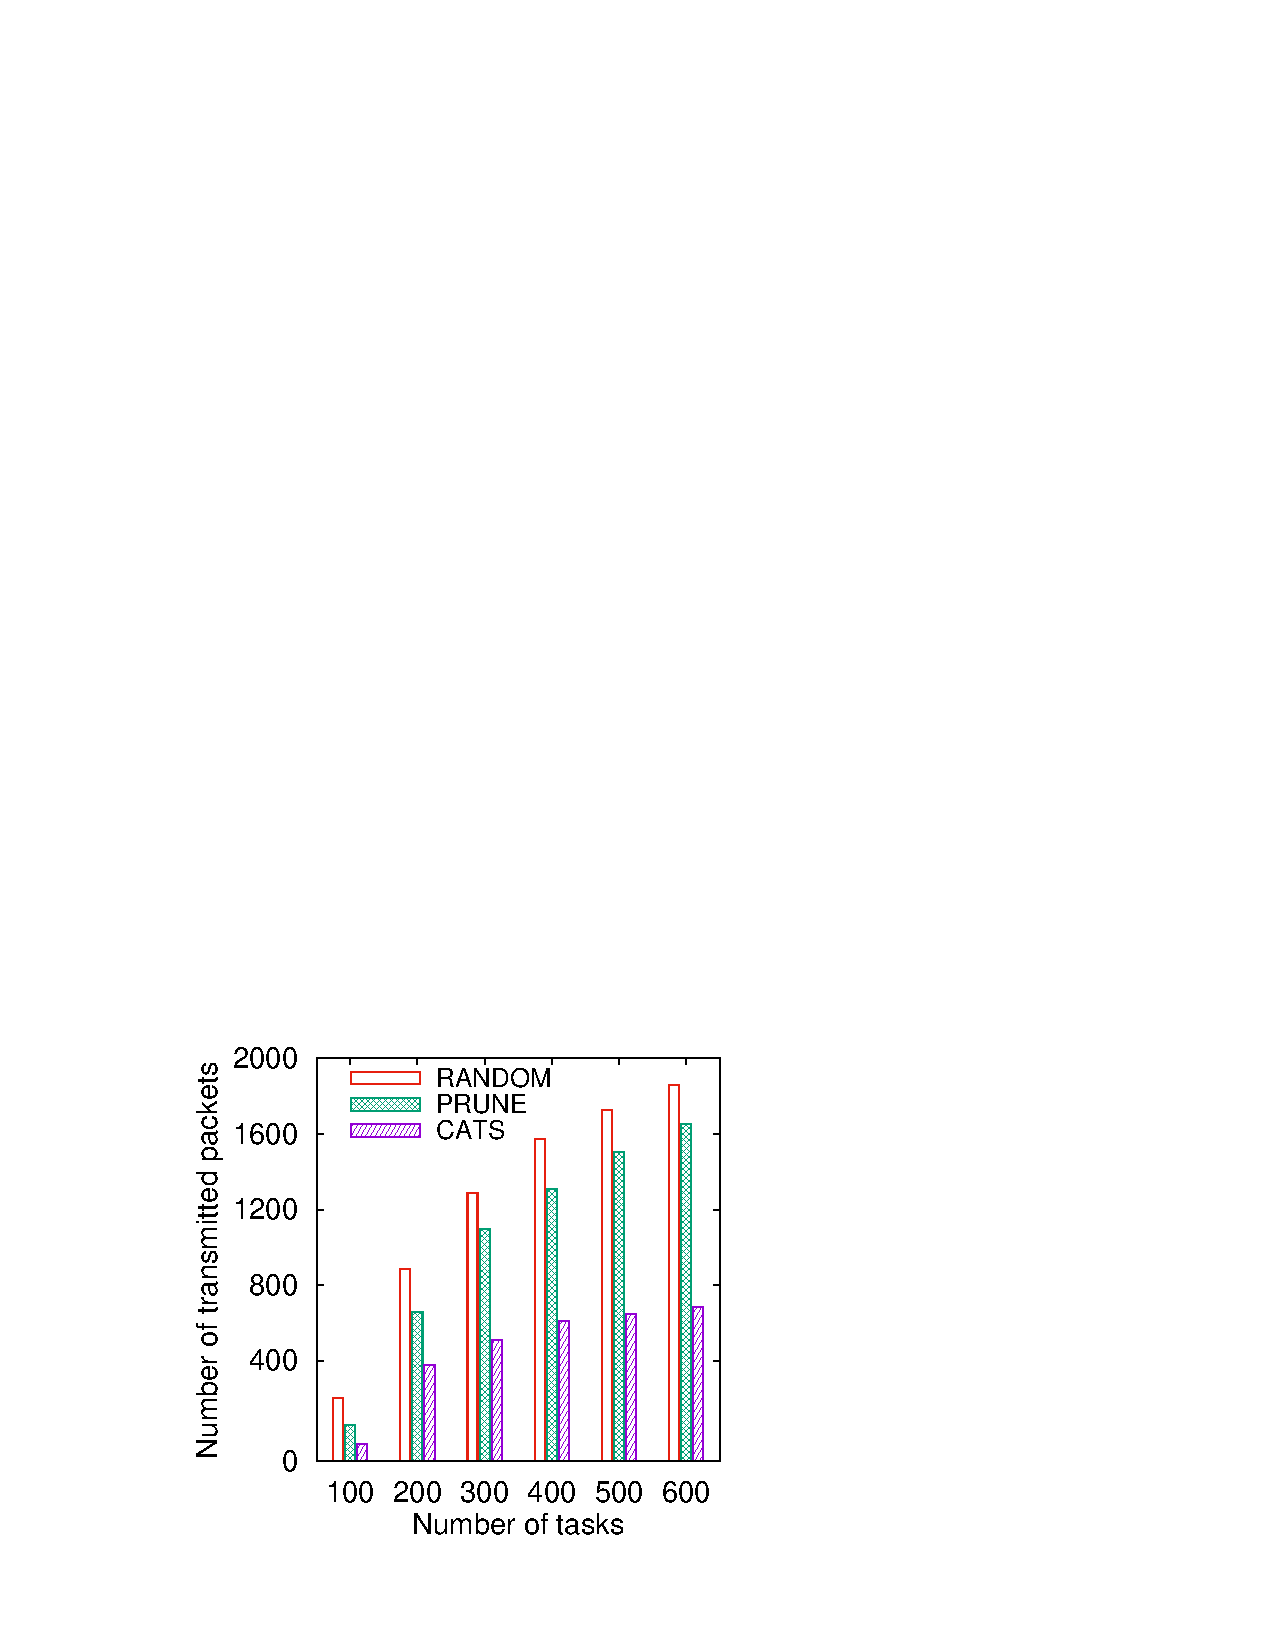
\includegraphics[width=0.254\columnwidth]{Figures/evaluation2_data_sampled_tasks}\label{evaluation2_data_sampled_tasks}}
\subfigure[$k\mathrm{=}8$, $n\mathrm{=}30$]{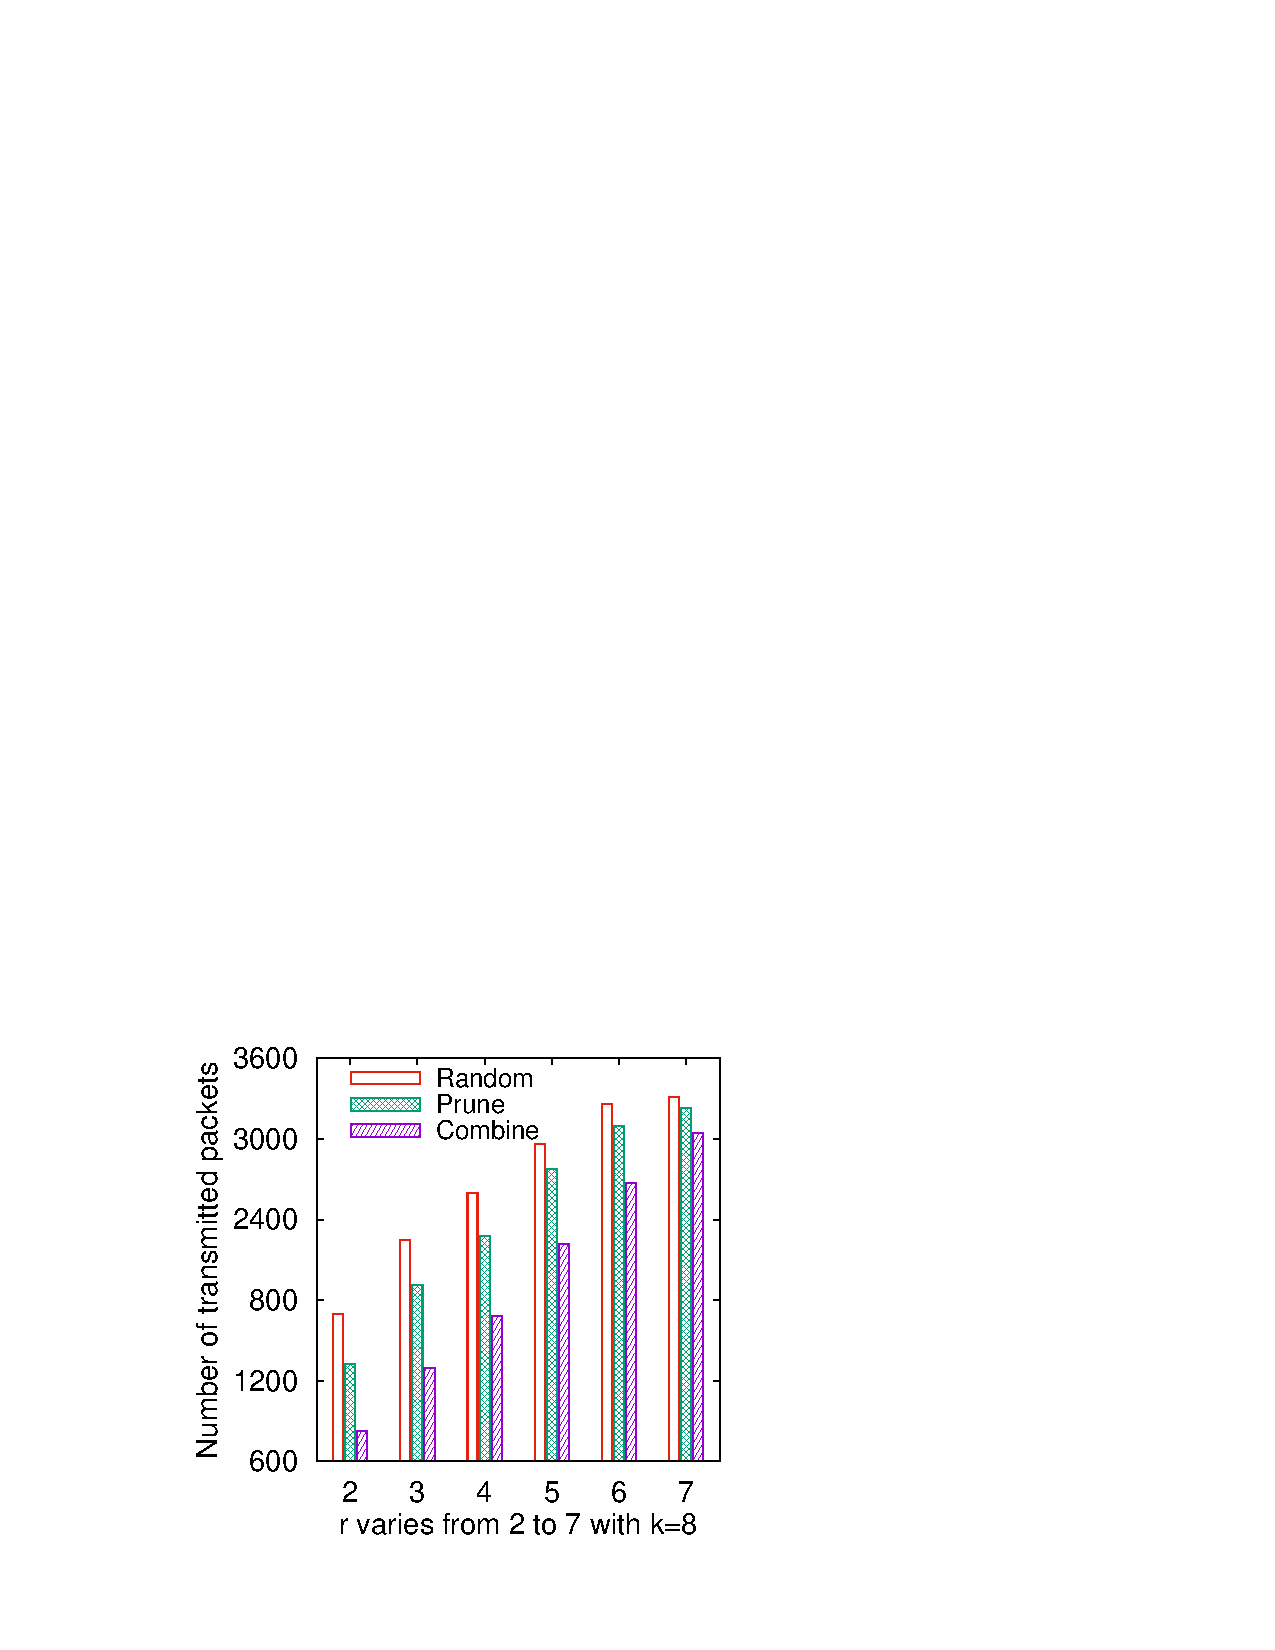
\includegraphics[width=0.252\columnwidth]{Figures/evaluation2_data_sampled_r}\label{evaluation2_data_sampled_r}}
\subfigure[$k\mathrm{=}5$, $r\mathrm{=}2$, $n\mathrm{=}5$]{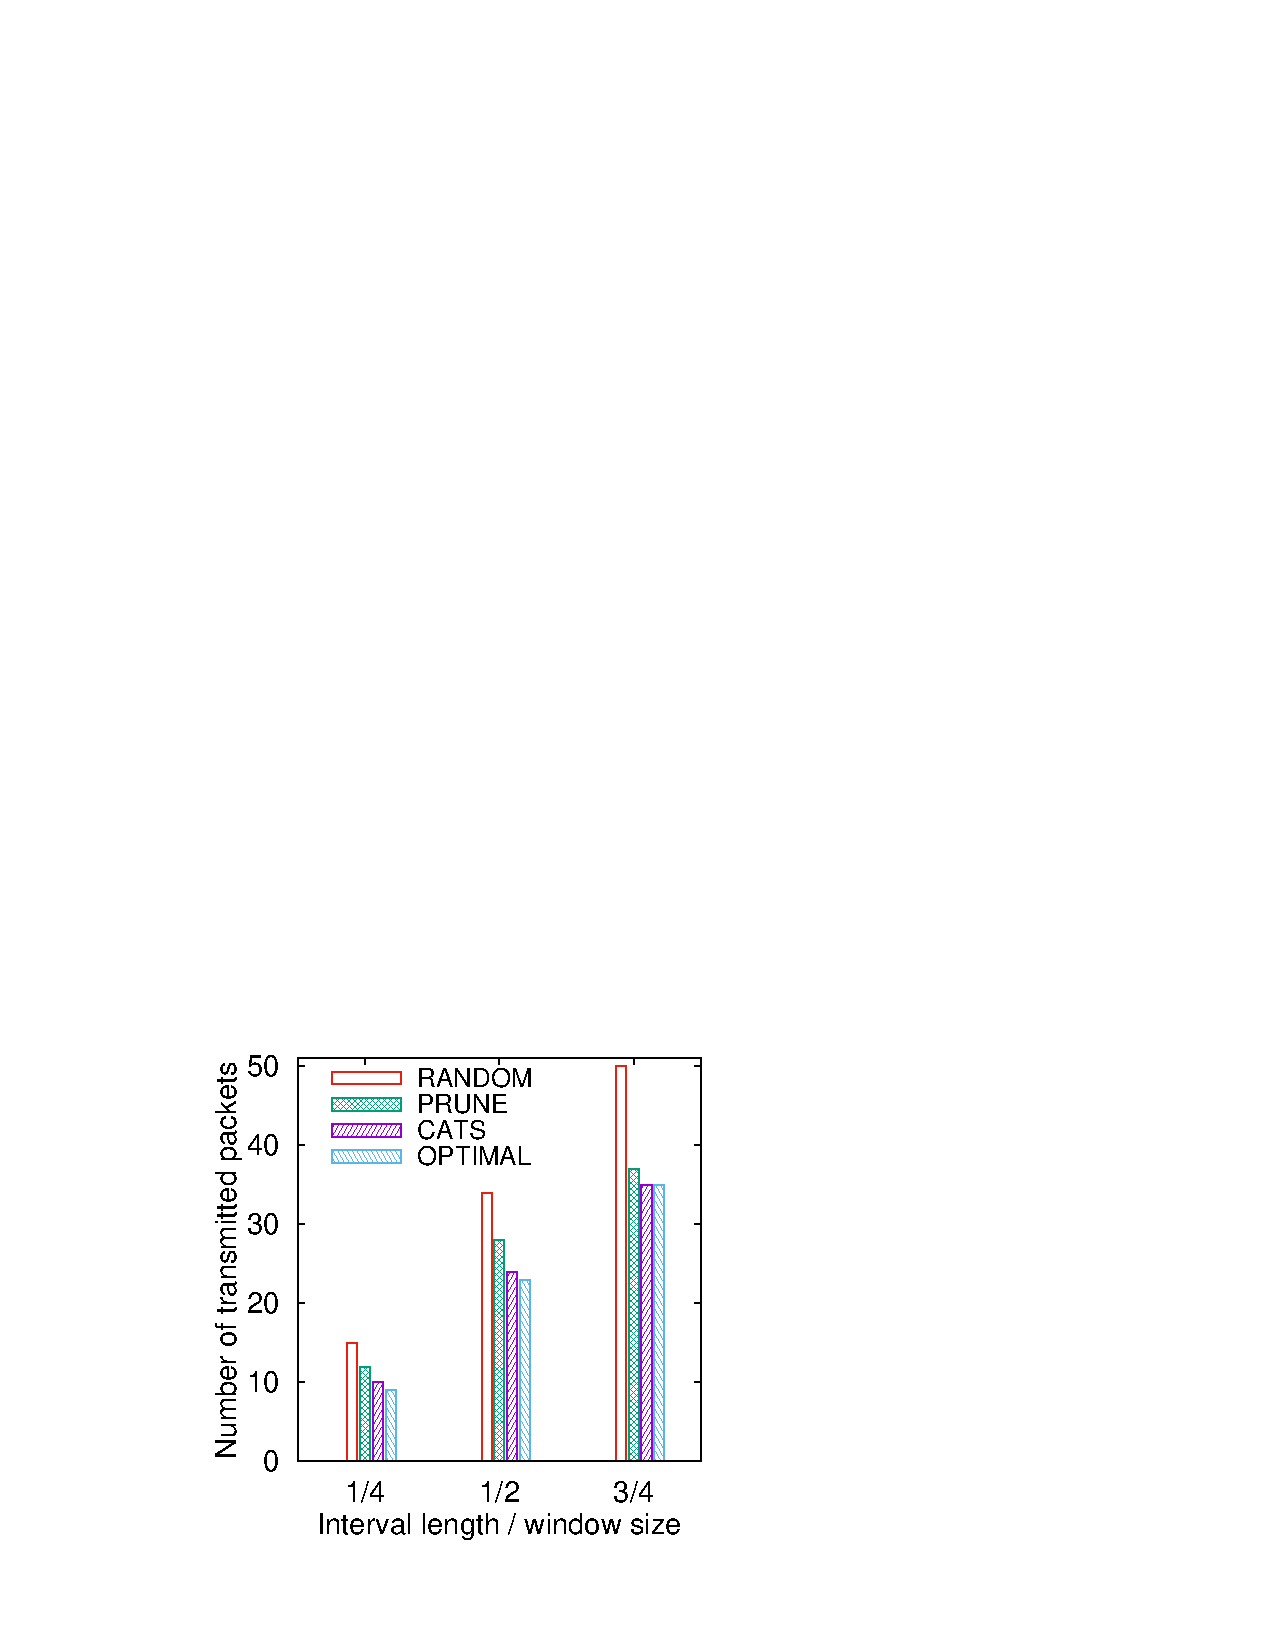
\includegraphics[width=0.234\columnwidth]{Figures/evaluation2_optimal1}\label{evaluation2_optimal1}}
\subfigure[$k\mathrm{=}8$, $n\mathrm{=}5$]{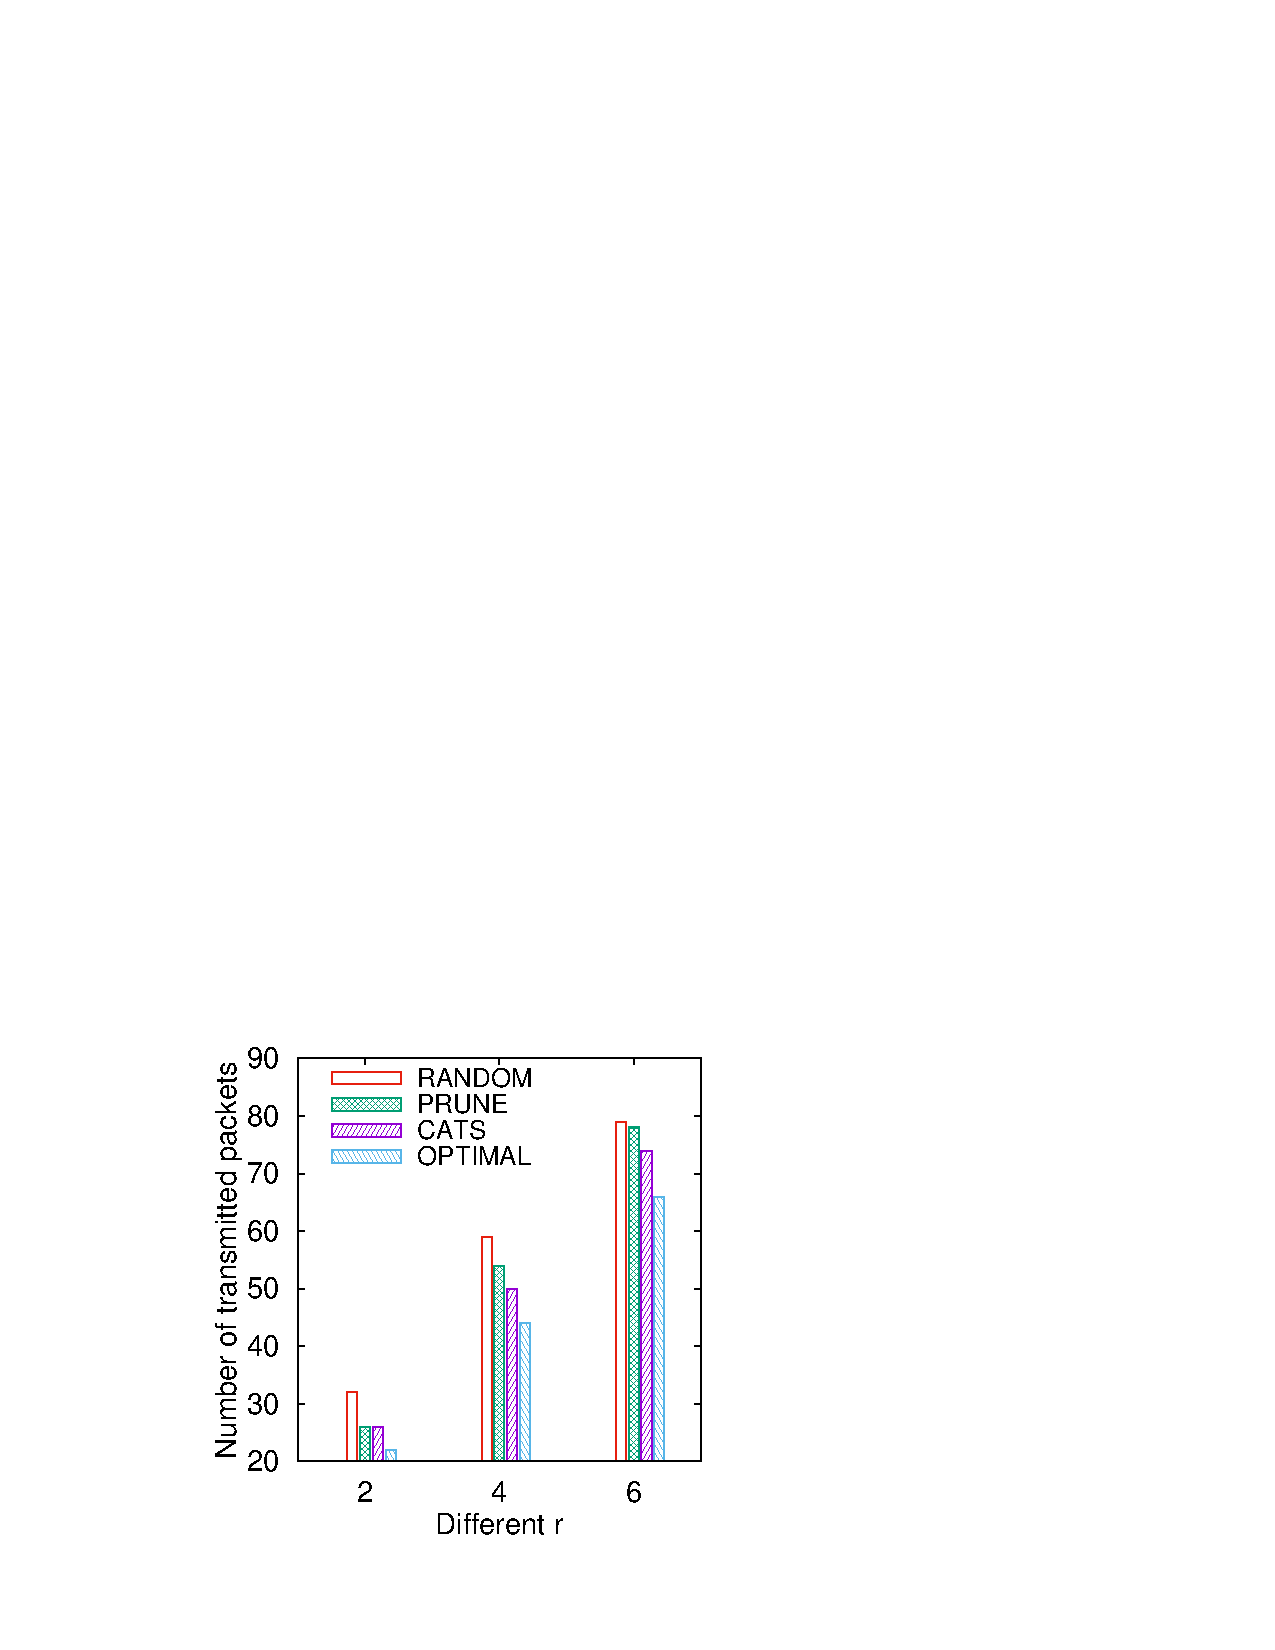
\includegraphics[width=0.236\columnwidth]{Figures/evaluation2_optimal2}\label{evaluation2_optimal2}}
%\renewcommand{\figurename}{abc}
\caption{A comparison of the number of transmitted packets by varying the number of tasks in (a) and the value of $r$ in (b). When the scale of tasks is limited, the number of transmitted packets is compared by varying the interval length of tasks in (c) and the value of $r$ in (d).}
\label{evaluation2}
\end{figure*}

%\begin{figure*}
%\centering
%\subfigure{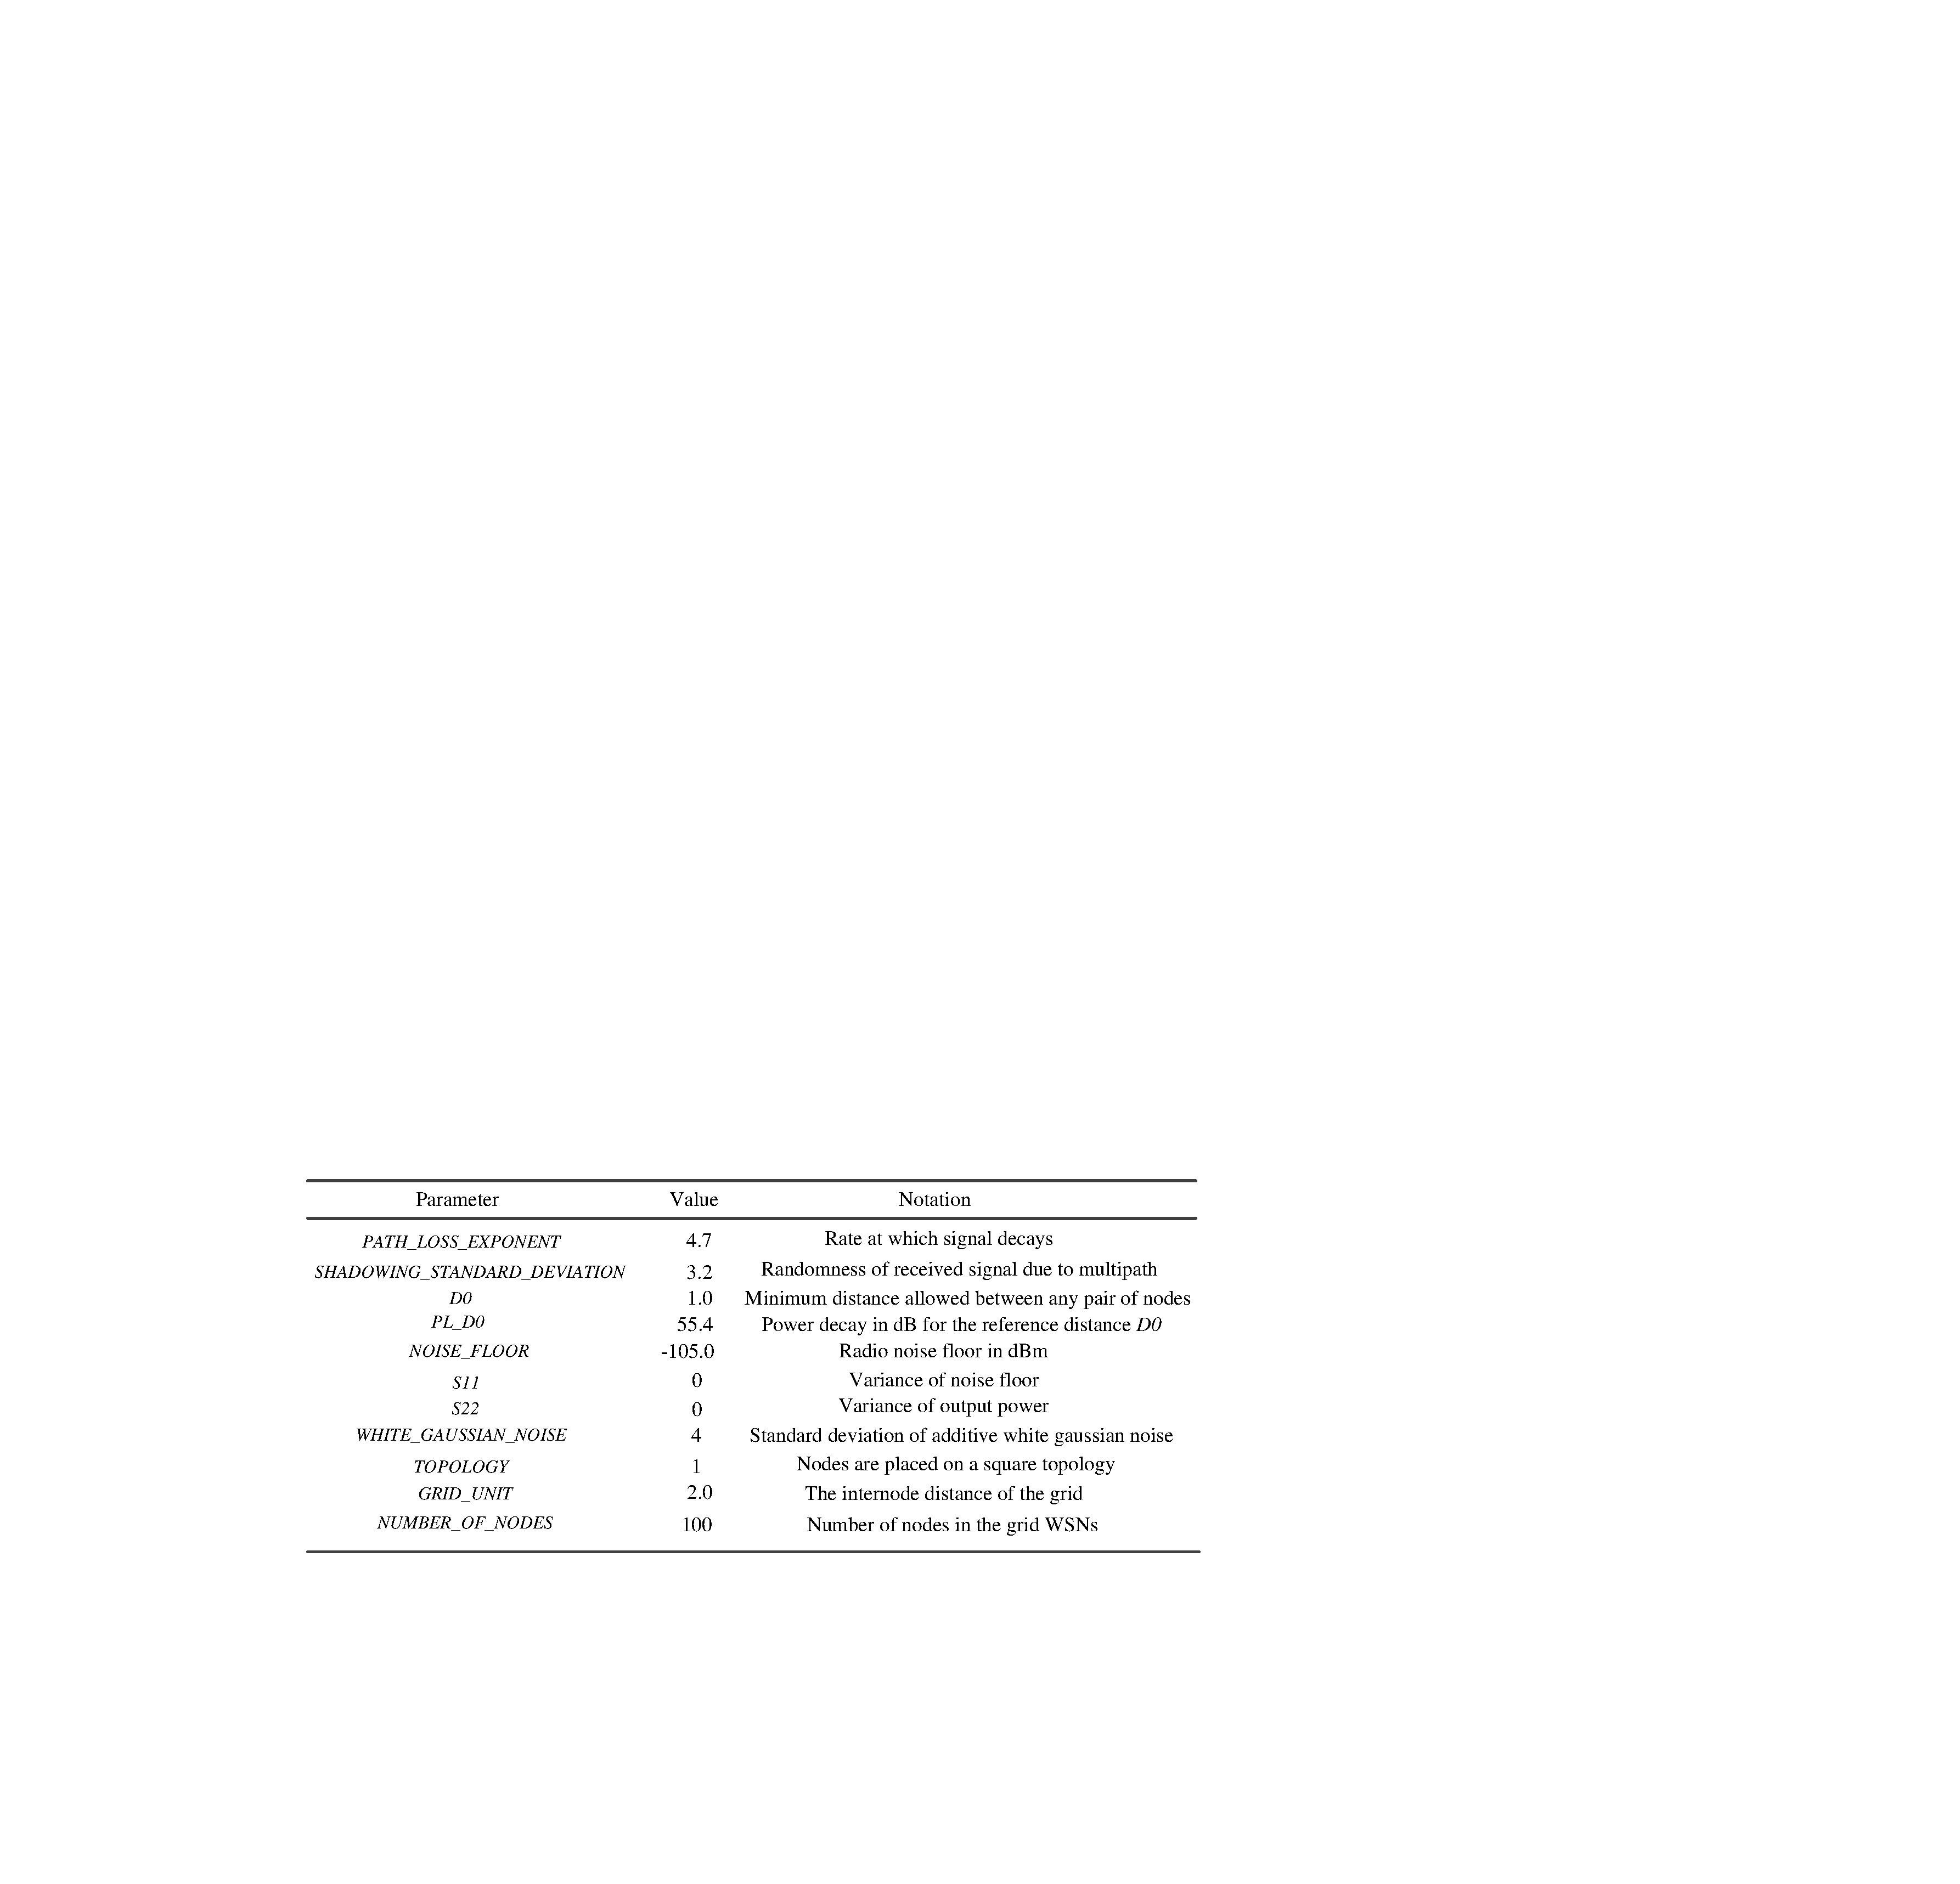
\includegraphics[width=1.6\columnwidth]{Figures/figure_appendix}}
%\caption{The parameter settings in the simulations by using TOSSIM. The left column is the parameters which can be used to configure a grid wireless sensor network, the middle column is the value, and the right column is the notions of these parameters.}
%\label{figure_appendix}
%\end{figure*}



In Fig. \ref{evaluation2_data_sampled_tasks}, we vary the number of sampling tasks in WSNs to compare the number of transmitted packets. By default, $k$ is set to $5$ and $r$ is set to $2$.  Fig. \ref{evaluation2_data_sampled_tasks} shows  the number of transmitted packets increases with the number of tasks. Moreover, methods \emph{Prune} and \emph{Combine} significantly decrease unnecessary sampled data than \emph{Random}, especially when the number of tasks grows. Precisely, when the cardinality of a task set is larger than $600$, the number of transmitted tasks produced by the \emph{Combine} seems to be half of that brought by \emph{Random}. In Fig. \ref{evaluation2_data_sampled_r}, we compare the number of transmitted packets by varying $r$ from $2$ to $6$ under the setting of  $k\mathrm{=}8$. It is obvious that both \emph{Prune} and \emph{Combine} reduce more transmitted packets than \emph{Random} does. Another observation is that the advantage of \emph{Prune} and \emph{Combine} becomes less significant when the growth of $r$. That is because when $r$ increases, more candidate sensor nodes are involved to be identified to execute a task. The randomness of \emph{Random} is weakened. Particularly, when $r$ equals $k$, \emph{Random} provides a deterministic allocation which shares the same performance with \emph{Combine}.

The task allocation problem amongst sensor nodes is difficult to derive an effective optimization solution. However, when the scale of tasks is small, we can find an optimal allocation solution by using a brute-force method. To evaluate the performance of our allocation rigorously, we compare the number of transmitted packets on each method by varying the number of tasks and the value of $r$. In Fig. \ref{evaluation2_optimal1}, we display three groups of tasks and each of which has five tasks. The interval length of a task is set to $1/4$, $1/2$, and $3/4$ of its window size in the group $1$, $2$, and $3$, respectively. These tasks appear in time slot $[0,\; 20]$ randomly. Here, $k\mathrm{=}5$, $r\mathrm{=}2$. It is clear that the number of transmitted packets increases with the  expansion of the interval length. However, \emph{Prune} and \emph{Combine} perform better than Random and are closely to the optimal allocation solution, i.e., \emph{Optimal}. This confirms the conclusion of  Theorem \ref{theorem_allocation} again which clarifies that our greedy allocation algorithm is a 2-factor approximation  of the optimal solution. In Fig. \ref{evaluation2_optimal2}, we set $k\mathrm{=}8$, and modify the value of $r$ from $2$ to $6$. A quick conclusion drawn from the figure illustrates that the number of transmitted packets increases with the growth of $r$. Under such condition,  the \emph{Combine} achieves greatly smaller number of transmitted packets than twice of that produced by the optimal solution. It verifies the conclusion of Theorem \ref{theorem_allocation} again.

\begin{figure*}[!t]
\centering
\subfigure[$k\mathrm{=}5$, $r\mathrm{=}2$, the testbed]{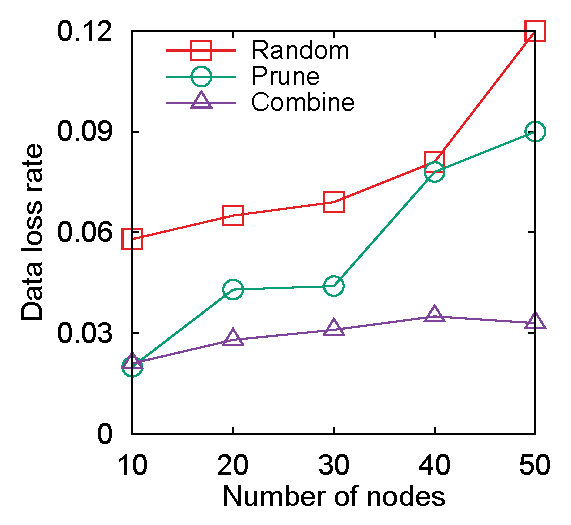
\includegraphics[width=0.256\columnwidth]{Figures/evaluation2_data_loss_rate}\label{evaluation2_data_loss_rate}}
\hspace{7pt}\subfigure[$k\mathrm{=}5$, $r\mathrm{=}2$, TOSSIM]{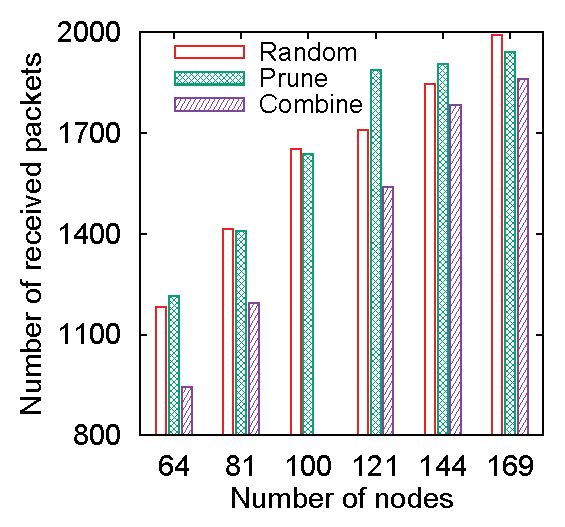
\includegraphics[width=0.255\columnwidth]{Figures/evaluation3_received_data}\label{evaluation3_received_data}}
\hspace{7pt}\subfigure[$k\mathrm{=}5$, $r\mathrm{=}2$, TOSSIM]{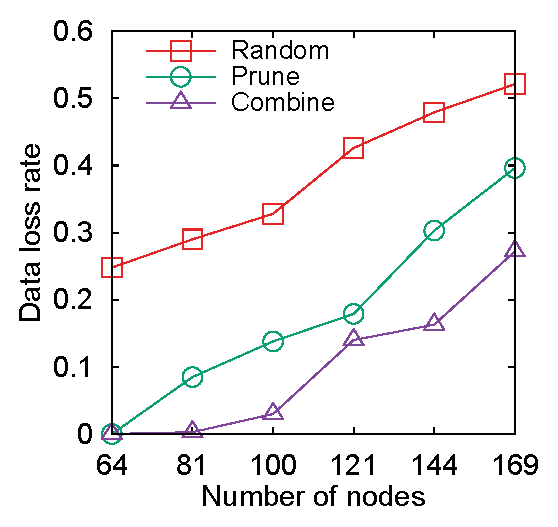
\includegraphics[width=0.255\columnwidth]{Figures/evaluation3_data_loss_rate}\label{evaluation3_loss_rate}}
\caption{A comparison of data loss rate in the testbed is presented by varying the number of nodes in (a). The number of received packets is compared by varying the number of nodes in (b) and so is the data loss rate in (c) for large scale wireless sensor networks simulated in TOSSIM.}
\label{evaluation3}
\end{figure*}

Large amount of  sampled data definitely leads to server delay and congestion  in WSNs, degrading the quality of data transmission as a result. In Fig. \ref{evaluation2_data_loss_rate}, we compare the data loss rate of every allocation method by changing the number of nodes in WSNs. It is obvious that the data loss rate becomes larger when the scale of network increases. But \emph{Prune} and \emph{Combine} significantly derive the smaller data loss rate than \emph{Random} does. This verifies the benefits of our allocation solution in improving the quality of data transmission by cutting down the unnecessary sampled data.

We conduct simulations for evaluating the scalability of our proposed algorithms for a large scale wireless sensor network. These simulations are implemented with TOSSIM which is a widely-used simulation tool for wireless sensor networks \cite{2003_TOSSIM}. We construct a grid network using the widely accepted settings in \cite{1999_wideband_channel_measurement}. As illustrated in Fig. \ref{evaluation3_received_data}, we compare the number of received data by varying the scale of the network. We apparently observe that \emph{Combine} brings smaller amount of received data than that \emph{Random} does. The reason is that \emph{Combine} reduces more unnecessary sampled data than \emph{Prune} and \emph{Random}. As illustrated in Fig. \ref{evaluation3_loss_rate}, the data loss rate in both \emph{Combine} and \emph{Prune} is much smaller than that in \emph{Random}. It happens when the number of transmitted data in \emph{Combine} and \emph{Prune} is smaller than that in \emph{Random}. In summary, \emph{Combine} is more suitable to be deployed for a large-scale wireless sensor network as it always performs much better than \emph{Random}.

\section{Discussion}
\label{discussion}
We have proposed methods of task allocation and scheduling of sampling interval and given much theoretical analysis about their performance. As the question is general, we aim to provide a universal solution which does not rely on the details of network. The sink node gets the strategy of task allocation in a wireless sensor network. It then allocates the sampling tasks to the sensor nodes. The allocation message will be added into packets and disseminated to sensor nodes with sampling tasks together. Comparing to the volume of sampled data of sampling tasks, such expenditure on the allocation solution is rather little. Meanwhile, as illustrated in Section \ref{section_performance_wsn}, adopting the strategy of task allocation can reduce redundancy of sampling data by more than 30\%. Therefore, it is worthy to trading little expenditure for appreciable data sharing. Besides, some other details  such as protocols of communication and data routing do not impact performance of the proposed algorithms. We do not adopt optimization on such communication protocols or routing strategy.


The allocation of tasks involves assigning each task to $r$ out of $k$ candidate sensor nodes. The current allocation scheme seeks to fully exploit the benefits of data sharing amongst tasks. In reality, there still exists other important constraints that can be exploited to improve the proposed allocation schemes. Note that each sensor node is resource-constrained, i.e., it has limited computation and memory resources. If a sensor node has been allocated many sampling tasks, it may not handle all the tasks timely and exhaust the energy at early time. This problem cannot thus be simply addressed by limiting the number of tasks a sensor node carries. The reason is that although different nodes have the same amount of sampling tasks, the real work load of  sensor nodes may have a considerable difference due to the data sharing strategy. Therefore, contemporary task allocation schemes can be more practical if we consider the load balance amongst sensor nodes. An effective method is to set a threshold for the constrained resource. Each allocation step makes sure that the threshold value is not exceeded. Algorithm \ref{allocation_prune} and Algorithm \ref{allocation_combine} are flexible to adjust for this tactics. When the  limited resource changes dynamically, the allocation problem will be more difficult to solve. We leave it as our future work.

In this paper, we aim to minimize the sampled data for a sampling task set by cooperatively allocating tasks and scheduling sampling interval of tasks which are allocated to a sensor node. Our proposed algorithms do not rely on the topology of a network. In fact, the information of a network can be used to improve the performance of our algorithms on many respects. For example, even though many applications require to get the entire data of sampling interval, we can divide the sampling interval into several segments for a $k$-coverage network if these segments can be integrated into the complete task finally on the sink node. These sampling segments can be allocated to the sensor nodes, which will help to balance the sampling workload on sensor nodes in our proposals. However, embedding the network information into our solutions introduces arduous problems, including task dividing, data fusion and so forth. We leave it as our future work as well.




\section{Conclusion}
\label{conclusion}
Many applications of WSNs  pursue to perform a set of interval data sampling tasks for decision-making.  In this paper, we focus on minimizing the interval data sampling in a $k$-coverage and $r$-redundant WSN. The solving of this optimal problem depends on the optimization of  two subproblems. The task allocation problem, MIN-SSA, allocates a sampling task to $r$ out of $k$ candidate nodes targeting at minimizing the amount of sampled data in the whole network. The scheduling problem, MIN-SA, schedules the sampling tasks targeting at minimizing the amount of sampled data on a single sensor node. We design a $2$-factor approximation scheduling and allocation method for each arduous problem. The effectiveness and scalability of our proposals is evaluated by employing a testbed and a widely-used simulation tool, i.e., TOSSIM, respectively. The evaluation results indicate that our methods significantly reduce the amount of sampled data, considerably save  precious energy and apparently improve the quality of communication due to the decrease of the data loss rate.

\begin{acks}
The work is partially supported by the National Natural Science Foundation of China (NSFC) under Grant 61402494, Grant 61402513, and Grant 61202487.
\end{acks}

%\bibliographystyle{IEEEtran}
%\bibliography{IEEEabrv,reference}
\bibliographystyle{ACM-Reference-Format-Journals}
\bibliography{reference}
%\clearpage
%\appendix[Parameter settings in the simulations with TOSSIM]

%\end{appendix}
\end{document}

